\documentclass{article}

\PassOptionsToPackage{numbers,sort&compress}{natbib}
\usepackage{tackling_climate_workshop_style}
\usepackage[utf8]{inputenc}
\usepackage[T1]{fontenc}
\usepackage{hyperref}
\hypersetup{hidelinks}
\usepackage{url}
\usepackage{graphicx}
\usepackage{booktabs}
\usepackage{tabularx}
\usepackage{array}
\usepackage{amsmath,amssymb}
\usepackage{microtype}
\usepackage{xcolor}
\usepackage{tikz}
\usetikzlibrary{arrows.meta,positioning,calc}

\definecolor{datablue}{HTML}{DCEAF7}
\definecolor{climorange}{HTML}{FCE3C3}
\definecolor{modelgreen}{HTML}{D9EAD3}
\definecolor{resultpurple}{HTML}{E7D9F2}
\definecolor{inkblue}{HTML}{365A73}
\definecolor{warmline}{HTML}{B46A2C}
\definecolor{metricblue}{HTML}{E8EEF3}
\newcolumntype{Y}{>{\raggedright\arraybackslash}X}
\newcommand{\rmse}{\operatorname{RMSE}}
\newcommand{\acc}{\operatorname{ACC}}

\title{Climatology Patching Exposes Cross-Variable Dependencies in AI Weather Forecasts}
\author{Anonymous Author(s)}

\begin{document}
\maketitle

\begin{abstract}
Forecast skill scores do not show which input fields a weather model needs or which fields it reconstructs from context. We audit this dependence without gradients by replacing one atmospheric input field with climatology matched by day of year and UTC hour, while holding the other inputs fixed. Repeating the intervention over 19 fields gives a directed $19\times19$ sensitivity matrix. Across 48 seasonally balanced initializations from 2024, the off-diagonal matrices of Aurora and Pangu-Weather correlate at $r=0.913$, yet individual dependencies are strongly asymmetric. At +6 h, patching $Z850$ changes $V850$ about nine times more than the reverse in both models. A six-point $Z1000$ dose sweep rises without saturation and separates the models: the $T1000$ slope falls from $0.690$ at +6 h to $0.217$ at +24 h for Aurora, but rises from $0.406$ to $0.614$ for Pangu-Weather. At full replacement, $T1000$ RMSE increases by $6.02\times$ and $3.35\times$, respectively, at +6 h. These values describe a finite stress test of a fixed model. They do not identify causal relations in the atmosphere.
\end{abstract}

\section{Introduction}

Pangu-Weather and Aurora produce global, high-resolution forecasts at low marginal cost~\citep{bi2023pangu,bodnar2025aurora}. Aggregate scores collapse their multivariate behavior into a few numbers. A model may achieve a similar score while relying on different input channels, reconstructing a missing field from neighboring levels, or propagating one bad field across many outputs. Forecast centers need this information before using a model in early-warning or climate-service workflows~\citep{wmo2025earlywarning}. Existing interpretation methods use gradients, perturbations, and representation analysis~\citep{yang2024survey}; gradients are expensive for billion-parameter global models, while correlations provide no direction of dependence.

We replace one input field with its expected seasonal and diurnal state, then measure which outputs move and how much. The study covers 19 inputs and outputs, Aurora and Pangu-Weather, and leads of 6 and 24 h. A continuous dose sweep checks whether the full replacement is a sensible endpoint, and spatial composites locate the added error. The method is an audit for forecast components used in adaptation and early warning; it does not perform climate attribution or estimate mitigation effects.

\section{Methods}

\subsection{Data, models, and sampling}

ERA5 provides initial states and verification truth~\citep{hersbach2020era5}; WeatherBench 2 climatology is matched by day of year and UTC hour and is computed over 1990--2019~\citep{rasp2024weatherbench2}. We evaluate Aurora (1.3B parameters; two input times) and Pangu-Weather (256M; one input time) on their $0.25^\circ$ grids. The audit uses 48 initializations in 2024: four dates per month, with 00/06/12/18 UTC balanced across the sample. The 19 audited fields are MSLP, 10-m $u/v$, 2-m temperature, and geopotential $Z$, specific humidity $Q$, temperature $T$, and $u/v$ wind at 1000, 850, and 500 hPa. Aurora's two input snapshots are both intervened upon.

\begin{figure}[t]
\centering
\resizebox{\linewidth}{!}{%
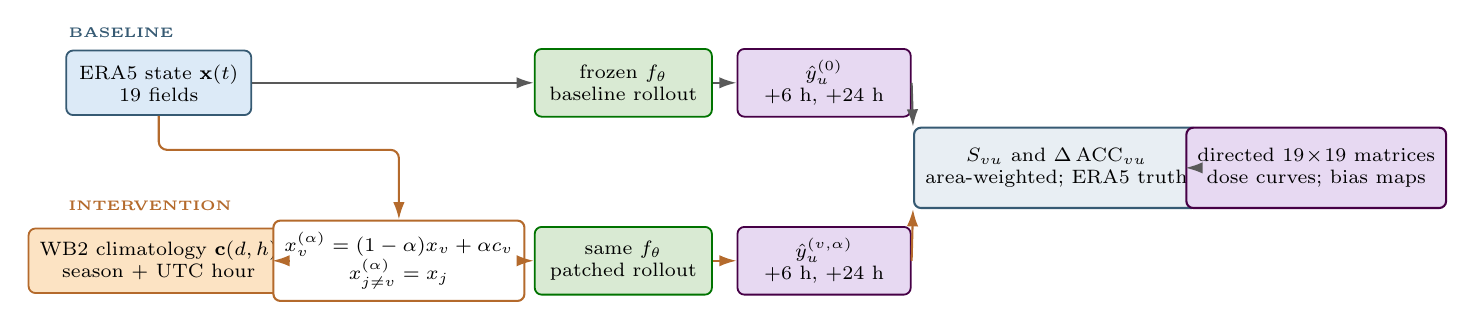
\begin{tikzpicture}[
  every node/.style={font=\scriptsize,align=center,inner sep=4pt},
  source/.style={draw=inkblue,rounded corners=2.5pt,fill=datablue,minimum width=2.35cm,minimum height=0.82cm,line width=0.65pt},
  clim/.style={draw=warmline,rounded corners=2.5pt,fill=climorange,minimum width=2.35cm,minimum height=0.82cm,line width=0.65pt},
  patch/.style={draw=warmline,rounded corners=2.5pt,fill=white,minimum width=3.10cm,minimum height=1.02cm,line width=0.75pt},
  model/.style={draw=green!45!black,rounded corners=2.5pt,fill=modelgreen,minimum width=2.25cm,minimum height=0.86cm,line width=0.65pt},
  forecast/.style={draw=violet!55!black,rounded corners=2.5pt,fill=resultpurple,minimum width=2.20cm,minimum height=0.86cm,line width=0.65pt},
  metric/.style={draw=inkblue,rounded corners=2.5pt,fill=metricblue,minimum width=2.65cm,minimum height=1.02cm,line width=0.75pt},
  result/.style={draw=violet!55!black,rounded corners=2.5pt,fill=resultpurple,minimum width=2.70cm,minimum height=1.02cm,line width=0.75pt},
  flow/.style={-{Latex[length=2.2mm,width=1.45mm]},draw=black!65,line width=0.75pt,rounded corners=3pt},
  patchflow/.style={flow,draw=warmline},
  lane/.style={font=\tiny\bfseries,anchor=west,inner sep=0pt}
]
  \node[lane,text=inkblue] at (-1.15,1.72) {BASELINE};
  \node[lane,text=warmline] at (-1.15,-0.48) {INTERVENTION};
  \node[source] (x) at (0,1.08) {ERA5 state $\mathbf{x}(t)$\\19 fields};
  \node[clim] (c) at (0,-1.18) {WB2 climatology $\mathbf{c}(d,h)$\\season + UTC hour};
  \node[model] (mb) at (5.90,1.08) {frozen $f_\theta$\\baseline rollout};
  \node[patch] (p) at (3.05,-1.18) {$x_v^{(\alpha)}=(1-\alpha)x_v+\alpha c_v$\\$x_{j\ne v}^{(\alpha)}=x_j$};
  \node[model] (mp) at (5.90,-1.18) {same $f_\theta$\\patched rollout};
  \node[forecast] (yb) at (8.45,1.08) {$\hat y_u^{(0)}$\\+6 h, +24 h};
  \node[forecast] (yp) at (8.45,-1.18) {$\hat y_u^{(v,\alpha)}$\\+6 h, +24 h};
  \node[metric] (m) at (11.40,0) {$S_{vu}$ and $\Delta\acc_{vu}$\\area-weighted; ERA5 truth};
  \node[result] (r) at (14.70,0) {directed $19\!\times\!19$ matrices\\dose curves; bias maps};
  \draw[flow] (x.east) -- (mb.west);
  \draw[flow] (mb.east) -- (yb.west);
  \draw[patchflow] (x.south) -- ++(0,-0.43) -| (p.north);
  \draw[patchflow] (c.east) -- (p.west);
  \draw[patchflow] (p.east) -- (mp.west);
  \draw[patchflow] (mp.east) -- (yp.west);
  \draw[flow] (yb.east) -- (m.north west);
  \draw[patchflow] (yp.east) -- (m.south west);
  \draw[flow] (m.east) -- (r.west);
\end{tikzpicture}}
\caption{Climatology patching uses paired rollouts. The date, model weights, and 18 untouched fields stay fixed. Full replacement ($\alpha=1$) supplies the matrix entry; six values of $\alpha$ trace the response.}
\label{fig:method}
\end{figure}

\subsection{Intervention and metrics}

For input field $v$, $P_v$ replaces that complete global field by climatology. For output field $u$, lead $\tau$, and initialization set $\mathcal D$, we report
\begin{align}
S_{vu}(\tau)&=\frac{1}{|\mathcal D|}\sum_{t\in\mathcal D}
\frac{\rmse_w(\hat y_u^{(v)},\hat y_u^{(0)})}{\sigma_w(y_u)}, \\
\Delta\acc_{vu}(\tau)&=\frac{1}{|\mathcal D|}\sum_{t\in\mathcal D}
\left[\acc_w(\hat y_u^{(v)},y_u,c_u)-\acc_w(\hat y_u^{(0)},y_u,c_u)\right].
\end{align}
All spatial sums use normalized $\cos\phi$ weights. $S$ measures forecast displacement; negative $\Delta\acc$ records a loss of verified anomaly skill. The dose experiment patches $Z1000$ at $\alpha\in\{0,.2,.4,.6,.8,1\}$ and reports $\rmse_w/\sigma_w(y-c)$, where one is the climatology no-skill reference. The intervention measures how the fitted network uses an input. It cannot establish atmospheric causality.

\section{Results}

\subsection{Correlation supplies a descriptive baseline}

The 69-channel Pangu output-anomaly matrix contains coherent vertical blocks for geopotential, humidity, temperature, and wind (Appendix~\ref{app:figures}). Its difference from ERA5 depends on the synoptic case. Single-time sliding-window correlations were also noisy on smooth fields. We retain both diagnostics as checks on association and use patching for directional analysis.

\begin{figure}[t]
\centering
\begin{minipage}[t]{0.485\linewidth}
  \centering
  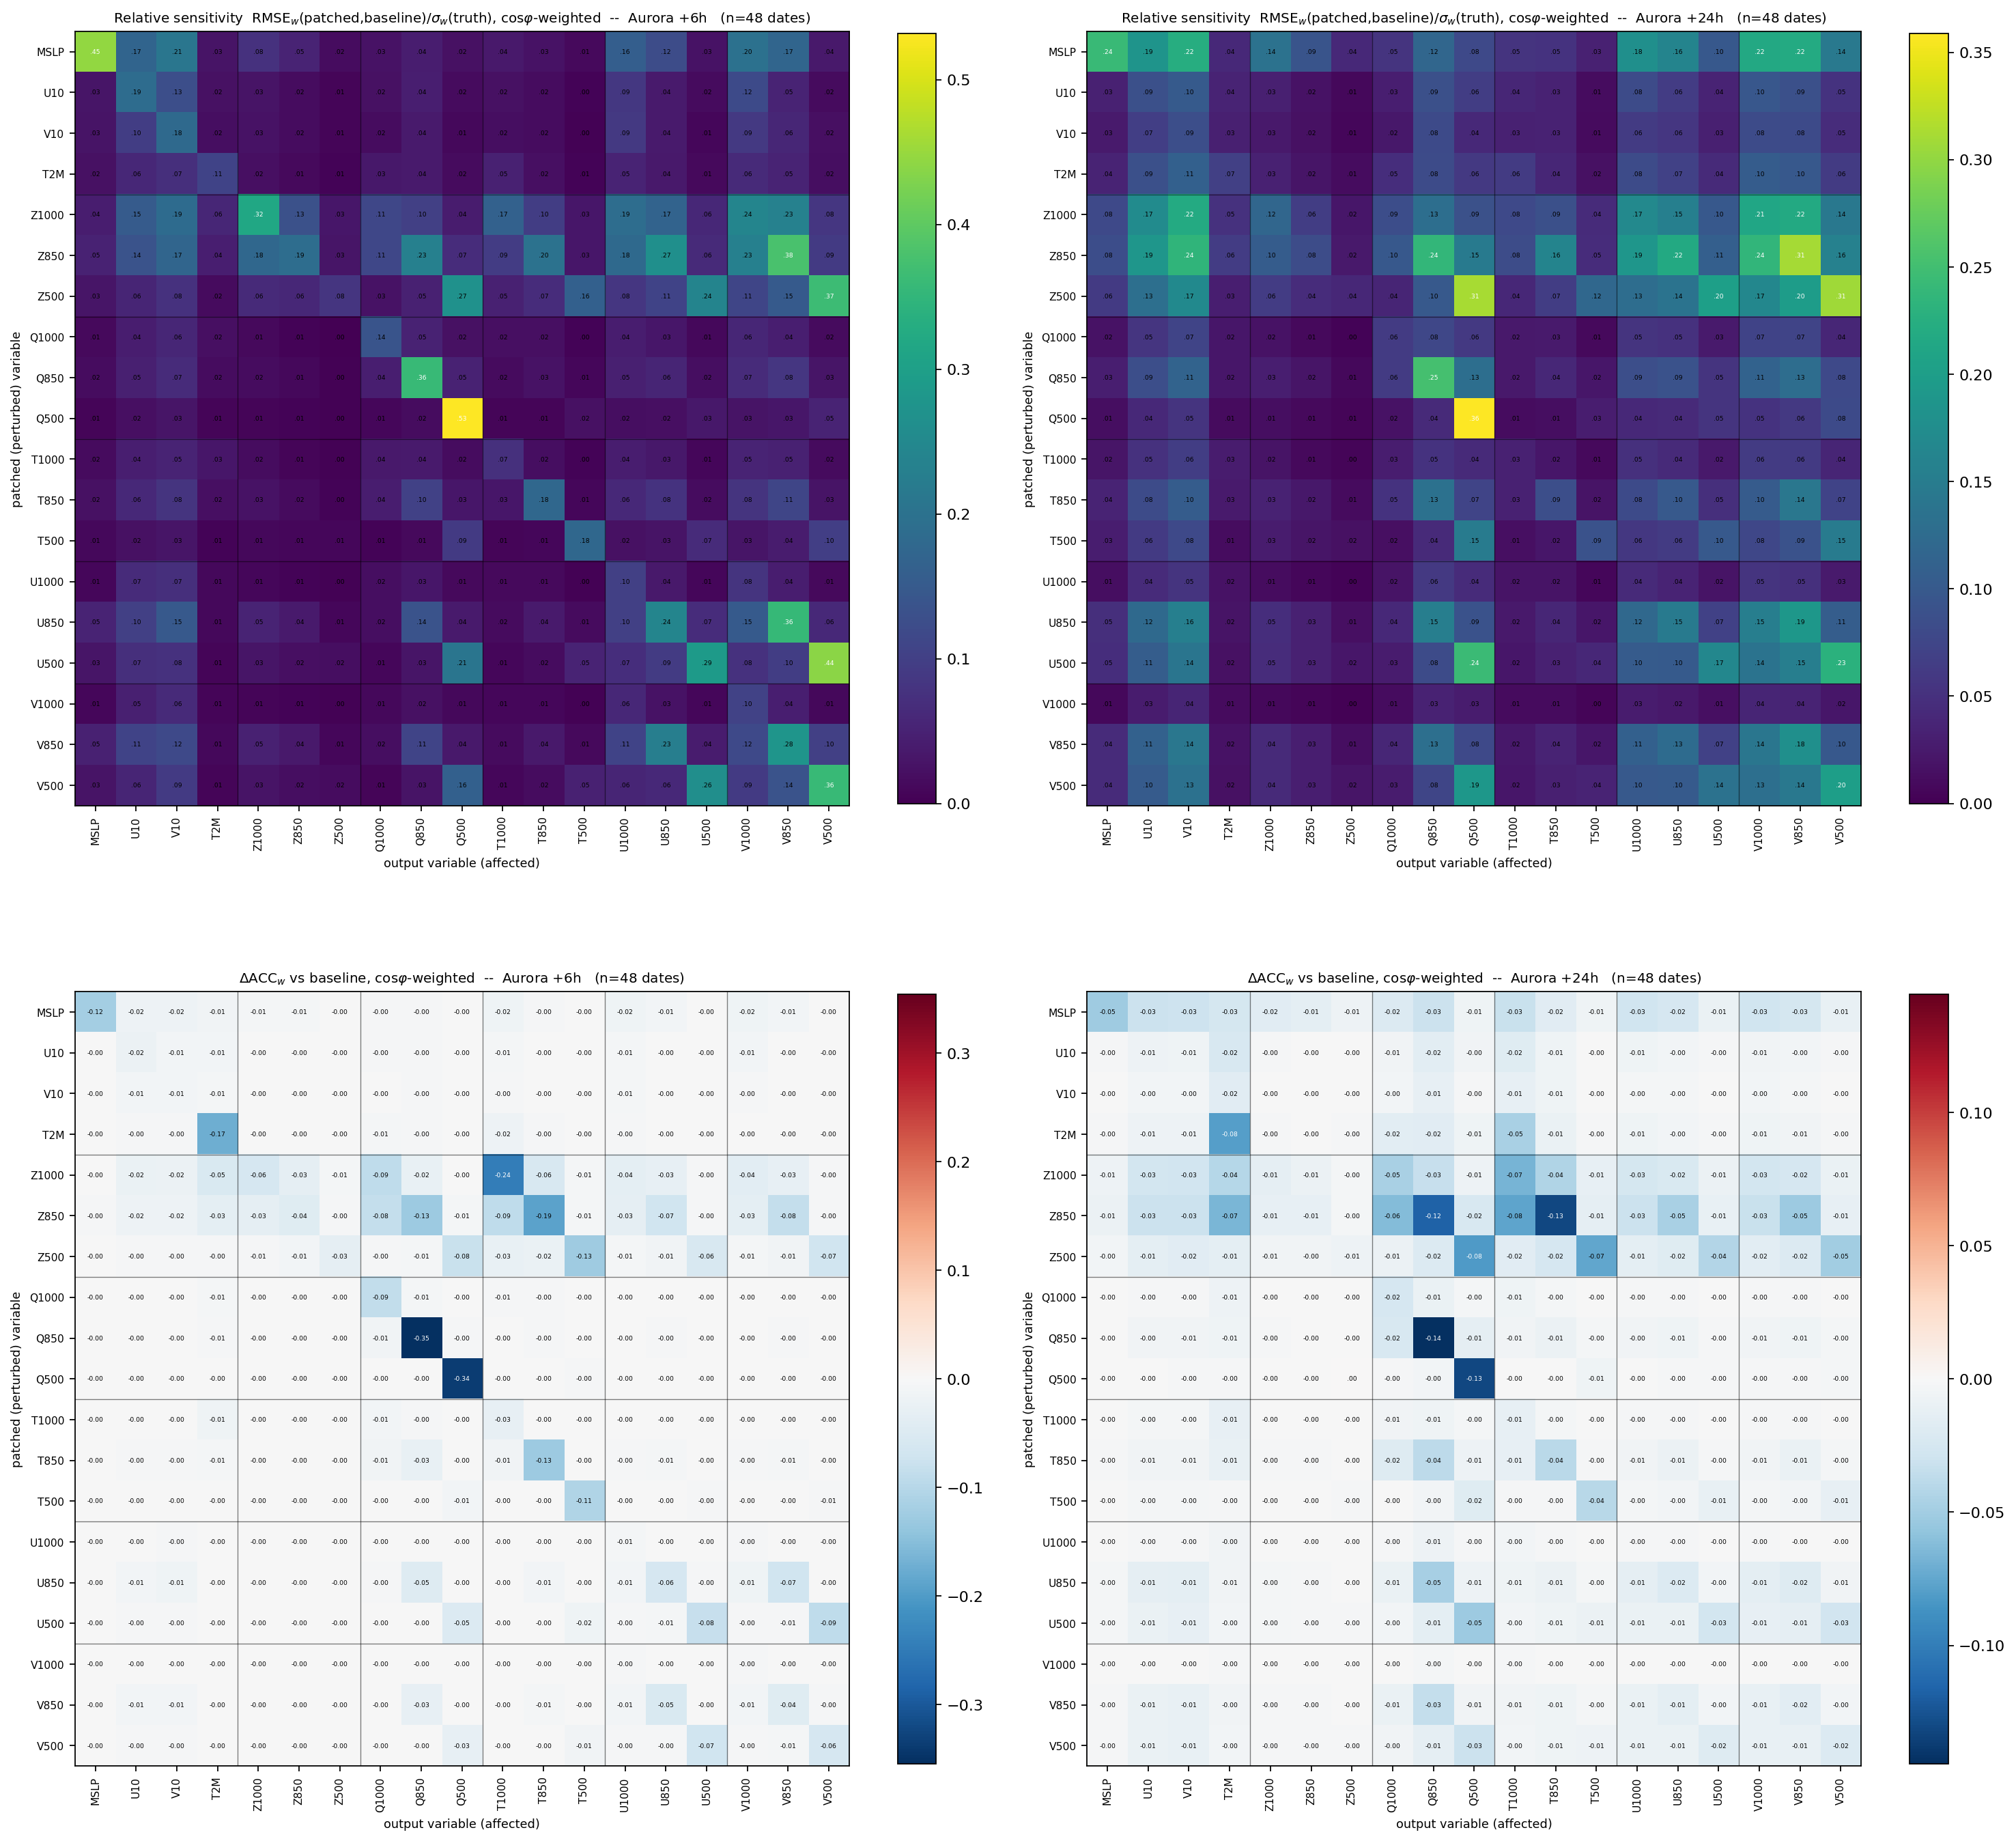
\includegraphics[width=\linewidth,trim=0.30in 8.65in 10.48in 0.12in,clip]{../../figures/patching_matrices/matrix_19var_aurora_n48_weighted.png}
  \\(a) Aurora, +6 h
\end{minipage}\hfill
\begin{minipage}[t]{0.485\linewidth}
  \centering
  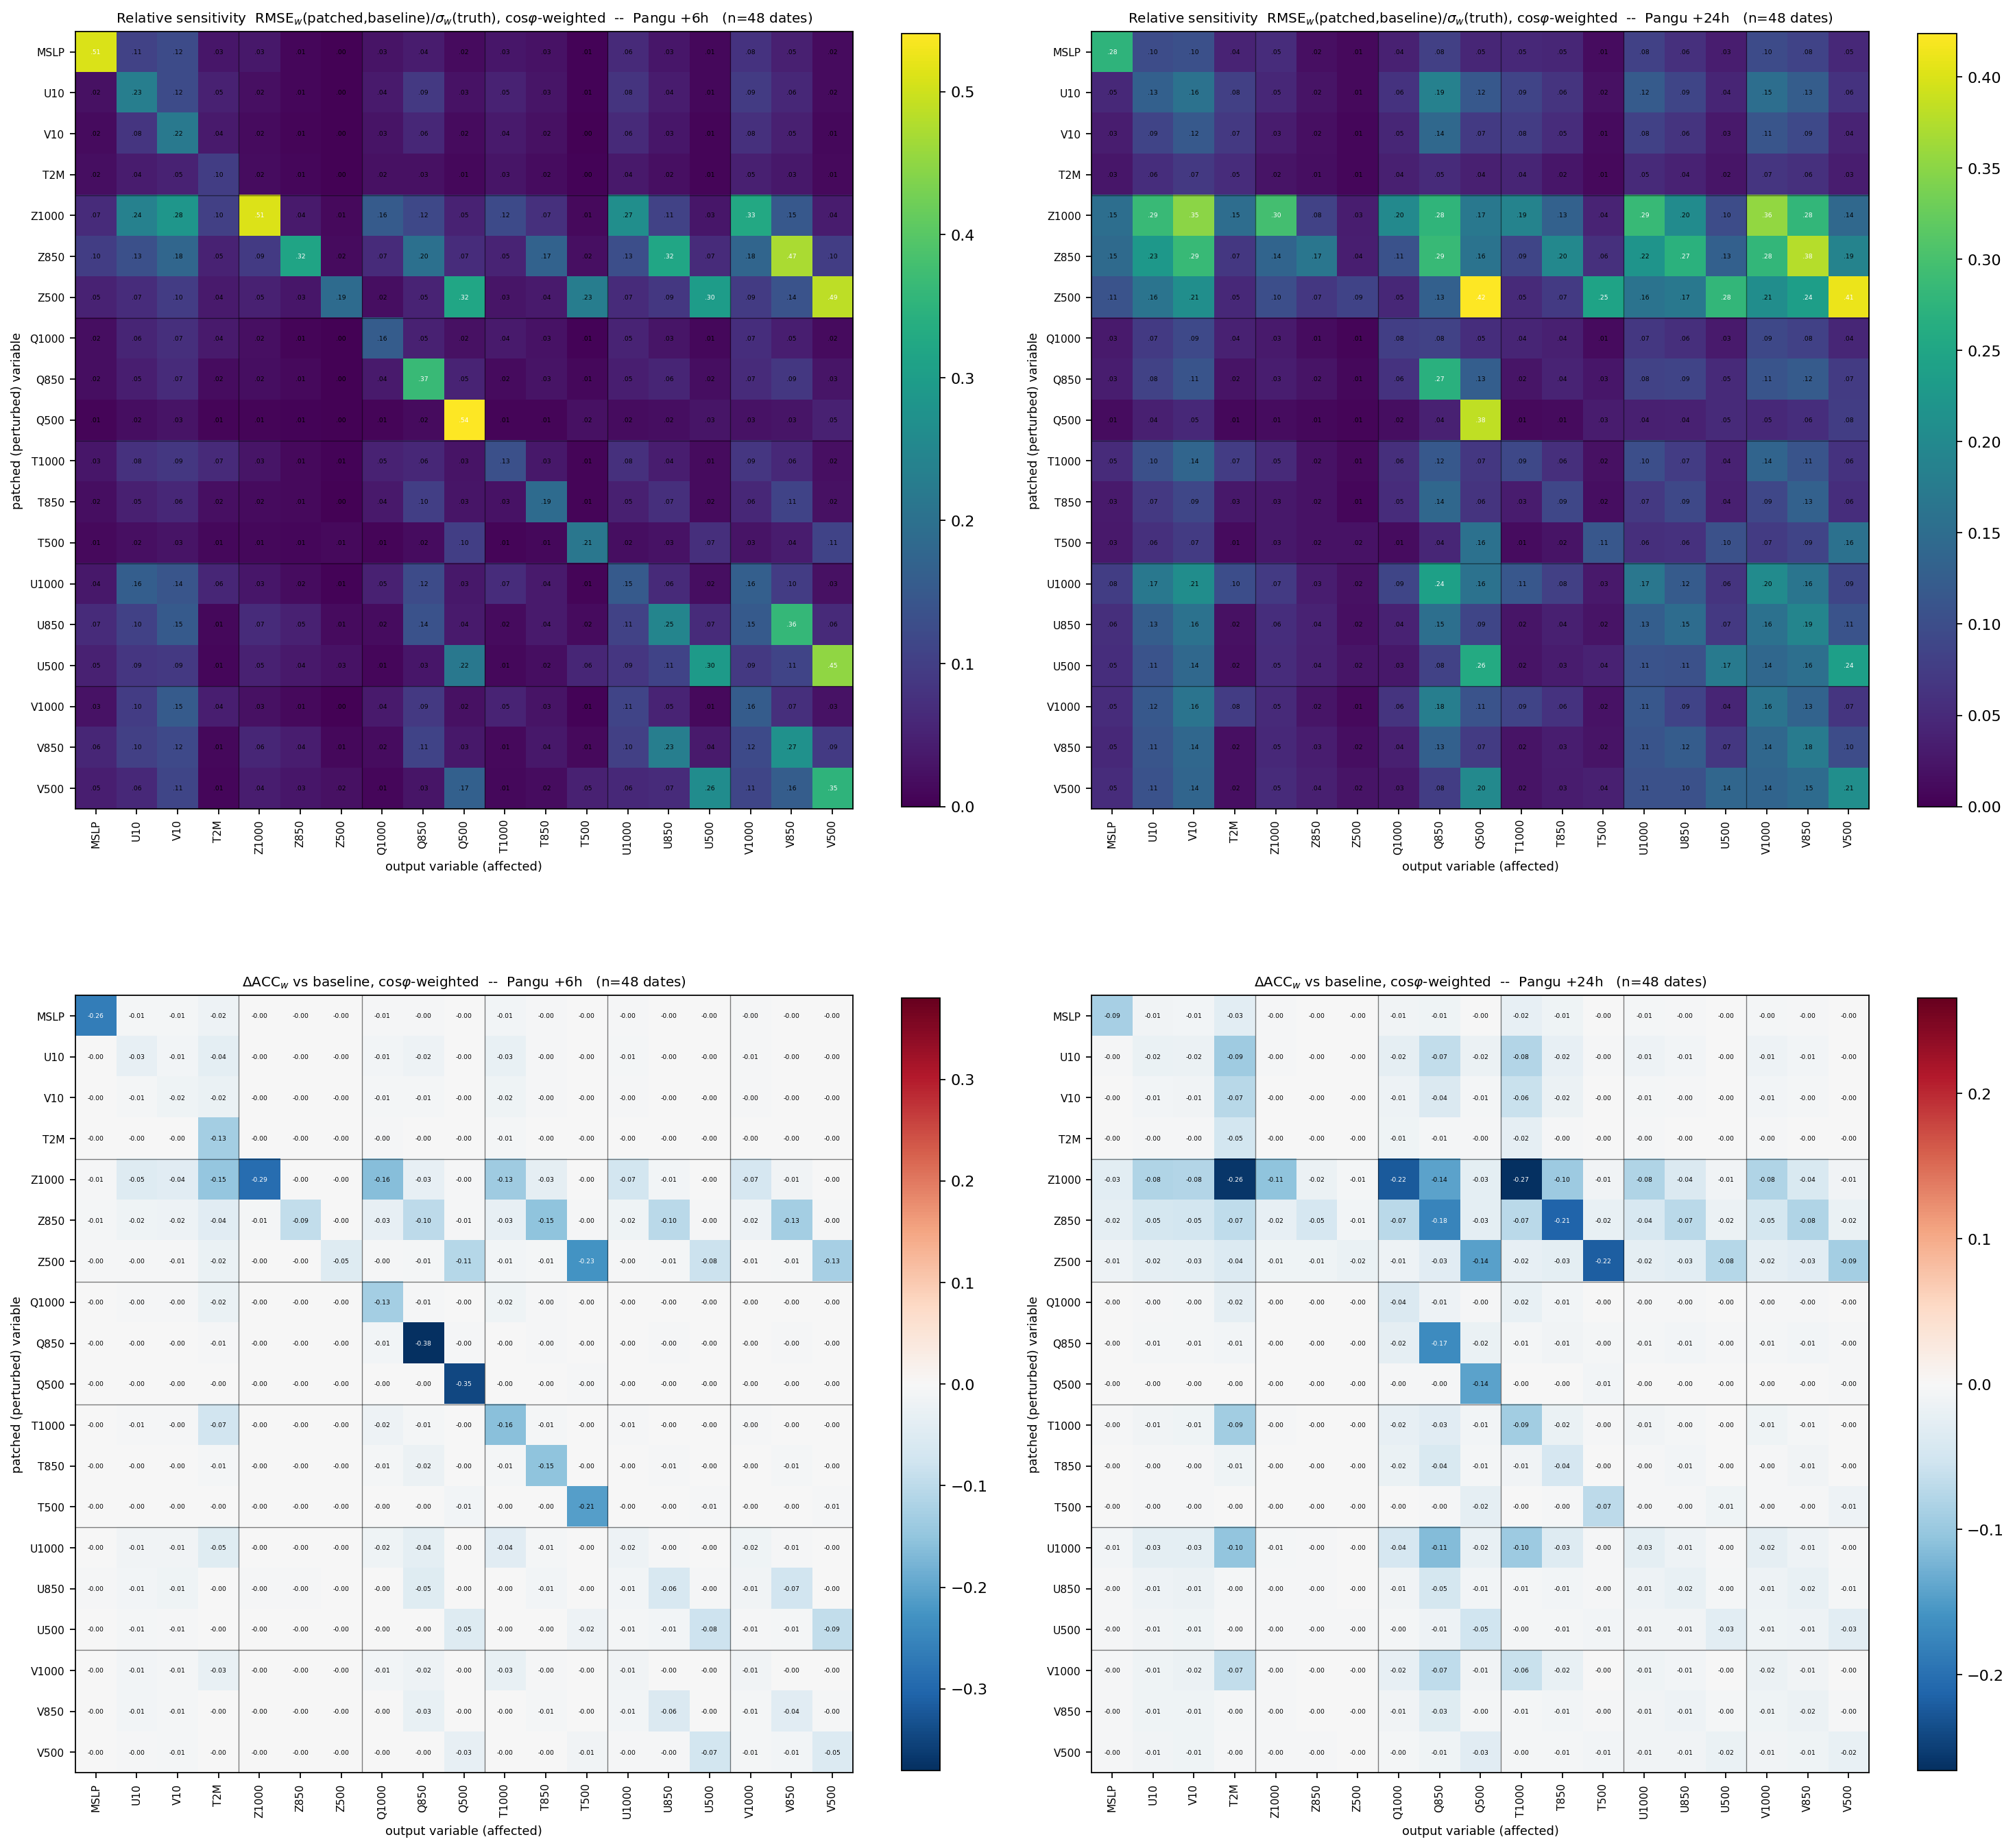
\includegraphics[width=\linewidth,trim=0.30in 8.65in 10.35in 0.12in,clip]{../../figures/patching_matrices/matrix_19var_pangu_n48_weighted.png}
  \\(b) Pangu-Weather, +6 h
\end{minipage}
\caption{Area-weighted directed sensitivity $S_{vu}$ for both models (row: patched input; column: affected output). The color scales are fitted separately, so comparisons should use the printed cell values. Full +6/+24 h sensitivity and $\Delta\acc$ panels appear in Appendix~\ref{app:figures}.}
\label{fig:matrixoverview}
\end{figure}

\subsection{Directed matrices reveal asymmetry and redundancy}

The off-diagonal entries of Aurora and Pangu correlate at $r=0.913$, but neither matrix is symmetric (Fig.~\ref{fig:matrixoverview}). At +6 h, $S_{Z850,V850}$ is $0.38$ for Aurora and $0.47$ for Pangu; the reverse entries are $0.04$ and $0.05$. The roughly ninefold contrast appears in both architectures. Diagonal entries distinguish fields that the network can reconstruct from context. Aurora gives $S_{Z500,Z500}=0.08$ and $S_{\mathrm{MSLP},\mathrm{MSLP}}=0.45$ at +6 h; Pangu gives $0.19$ and $0.53$. These values support redundancy in $Z500$ and stronger unique dependence on MSLP, especially for Aurora.

\begin{table}[t]
\caption{Main results, averaged over 48 dates. The repository stores point estimates but no date-block confidence intervals.}
\label{tab:results}
\centering
\small
\begin{tabularx}{\linewidth}{@{}p{0.27\linewidth}Y Y@{}}
\toprule
Diagnostic & Evidence & Interpretation \\
\midrule
Cross-model structure & off-diagonal $r=0.913$ & many dependencies recur across architectures \\
Direction at +6 h & $Z850\!\to V850$: $0.38/0.47$; reverse: $0.04/0.05$ (Aurora/Pangu) & mass-to-wind dependence is about ninefold stronger \\
Diagonal contrast at +6 h & $Z500$: $0.08/0.19$; MSLP: $0.45/0.53$ & MSLP is less recoverable from context \\
$T1000$ dose slope & Aurora: $0.690\to0.217$; Pangu: $0.406\to0.614$ (+6$\to$+24 h) & lead-time behavior differs by model \\
$T1000$ spatial RMSE & Aurora: $6.02\times/2.01\times$; Pangu: $3.35\times/3.06\times$ (+6/+24 h) & the response covers 99--100\% of grid cells \\
\bottomrule
\end{tabularx}
\end{table}

\subsection{Dose response separates the models}

All six $Z1000$ dose points rise, with no plateau before $\alpha=1$. For Aurora at +6 h, the fitted slopes are $0.690$ for $T1000$, $0.274$ for $Q1000$, and $0.180/0.187$ for $U/V1000$. The $T1000$ slope falls to $0.217$ at +24 h. Pangu follows a different lead-time pattern: its $T1000$ slope rises from $0.406$ to $0.614$, and its $T2M$ slope rises from $0.387$ to $0.570$. The full replacement therefore ranks finite model sensitivity, while the intermediate points show why it should not be read as an infinitesimal Jacobian.

\subsection{Spatial composites show persistent, model-specific error}

The $T1000$ composite in Fig.~\ref{fig:bias} reports temporal RMSE at every grid cell, patched minus baseline. At +6 h, full $Z1000$ replacement raises the global mean of per-cell $T1000$ RMSE by $6.02\times$ for Aurora and $3.35\times$ for Pangu. At +24 h, the ratios are $2.01\times$ and $3.06\times$. The increase covers 99--100\% of cells. Aurora weakens markedly by +24 h; Pangu retains most of its response. Both maps concentrate large increments in mid and high latitudes, while Pangu shows broader tropical and subtropical increments.

\begin{figure}[t]
\centering
\begin{minipage}[t]{0.485\linewidth}
  \centering
  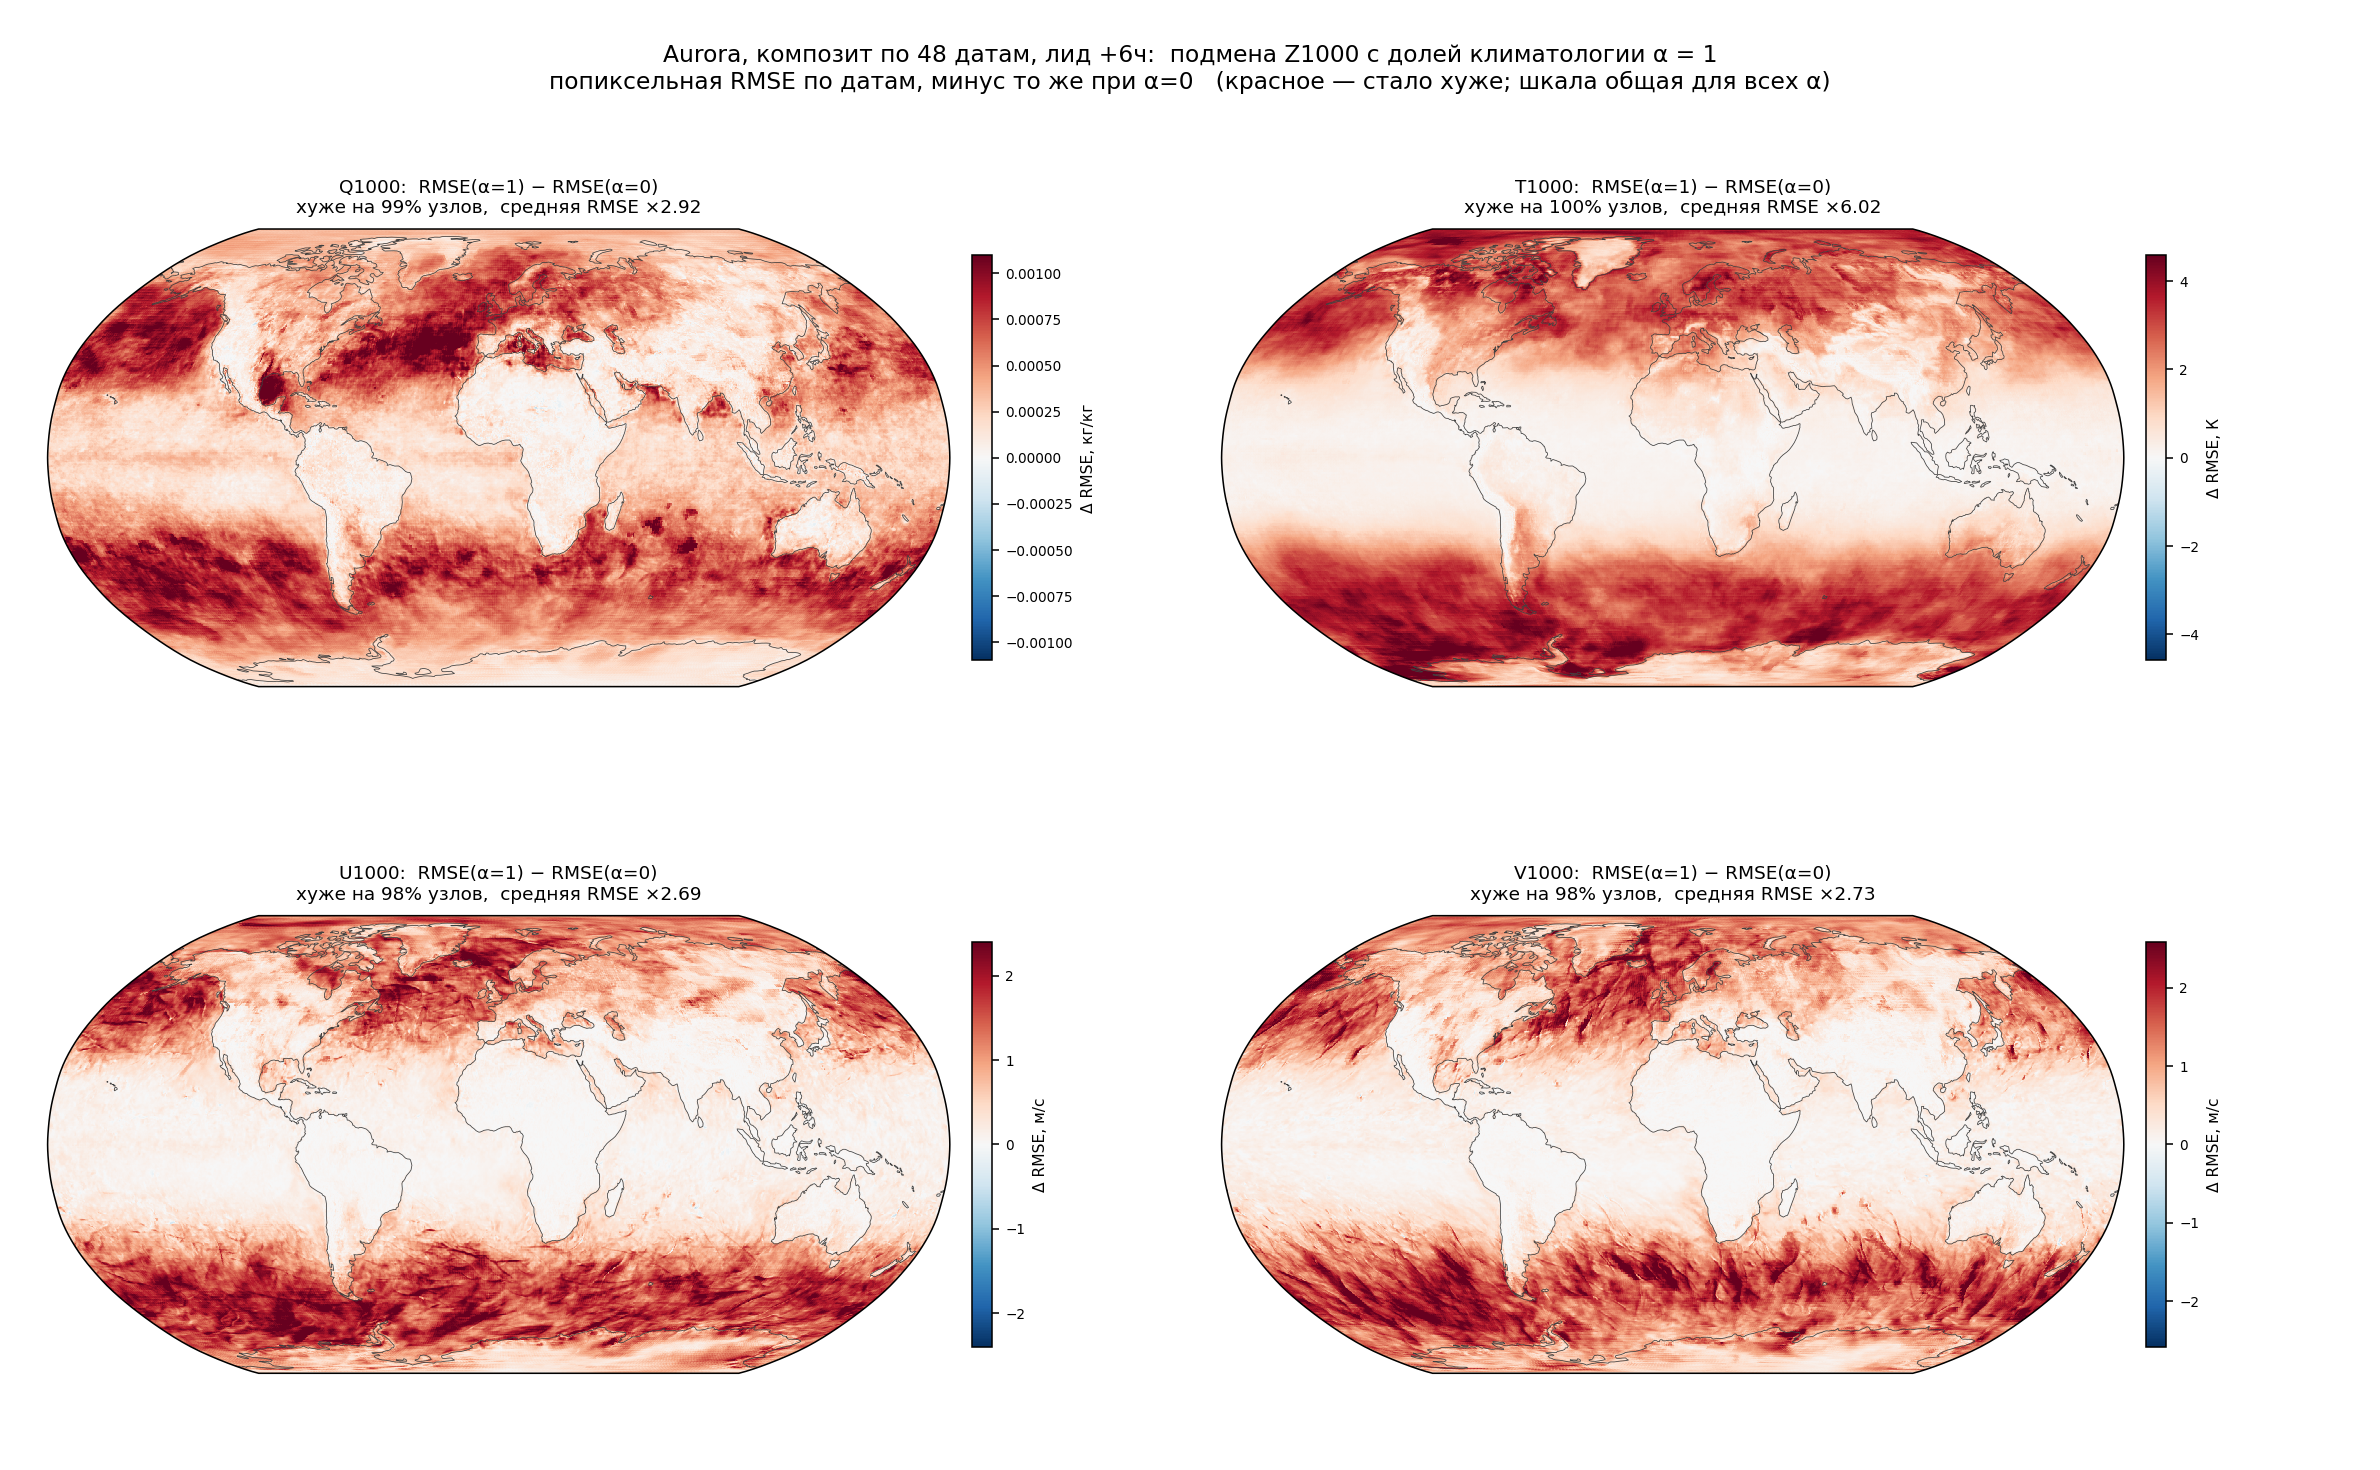
\includegraphics[width=\linewidth,trim=8.10in 5.55in 0.20in 1.58in,clip]{../../figures/bias_maps/composite_bias_Z1000_lead6_alpha1_n48.png}
  \\(a) Aurora, +6 h: $6.02\times$
\end{minipage}\hfill
\begin{minipage}[t]{0.485\linewidth}
  \centering
  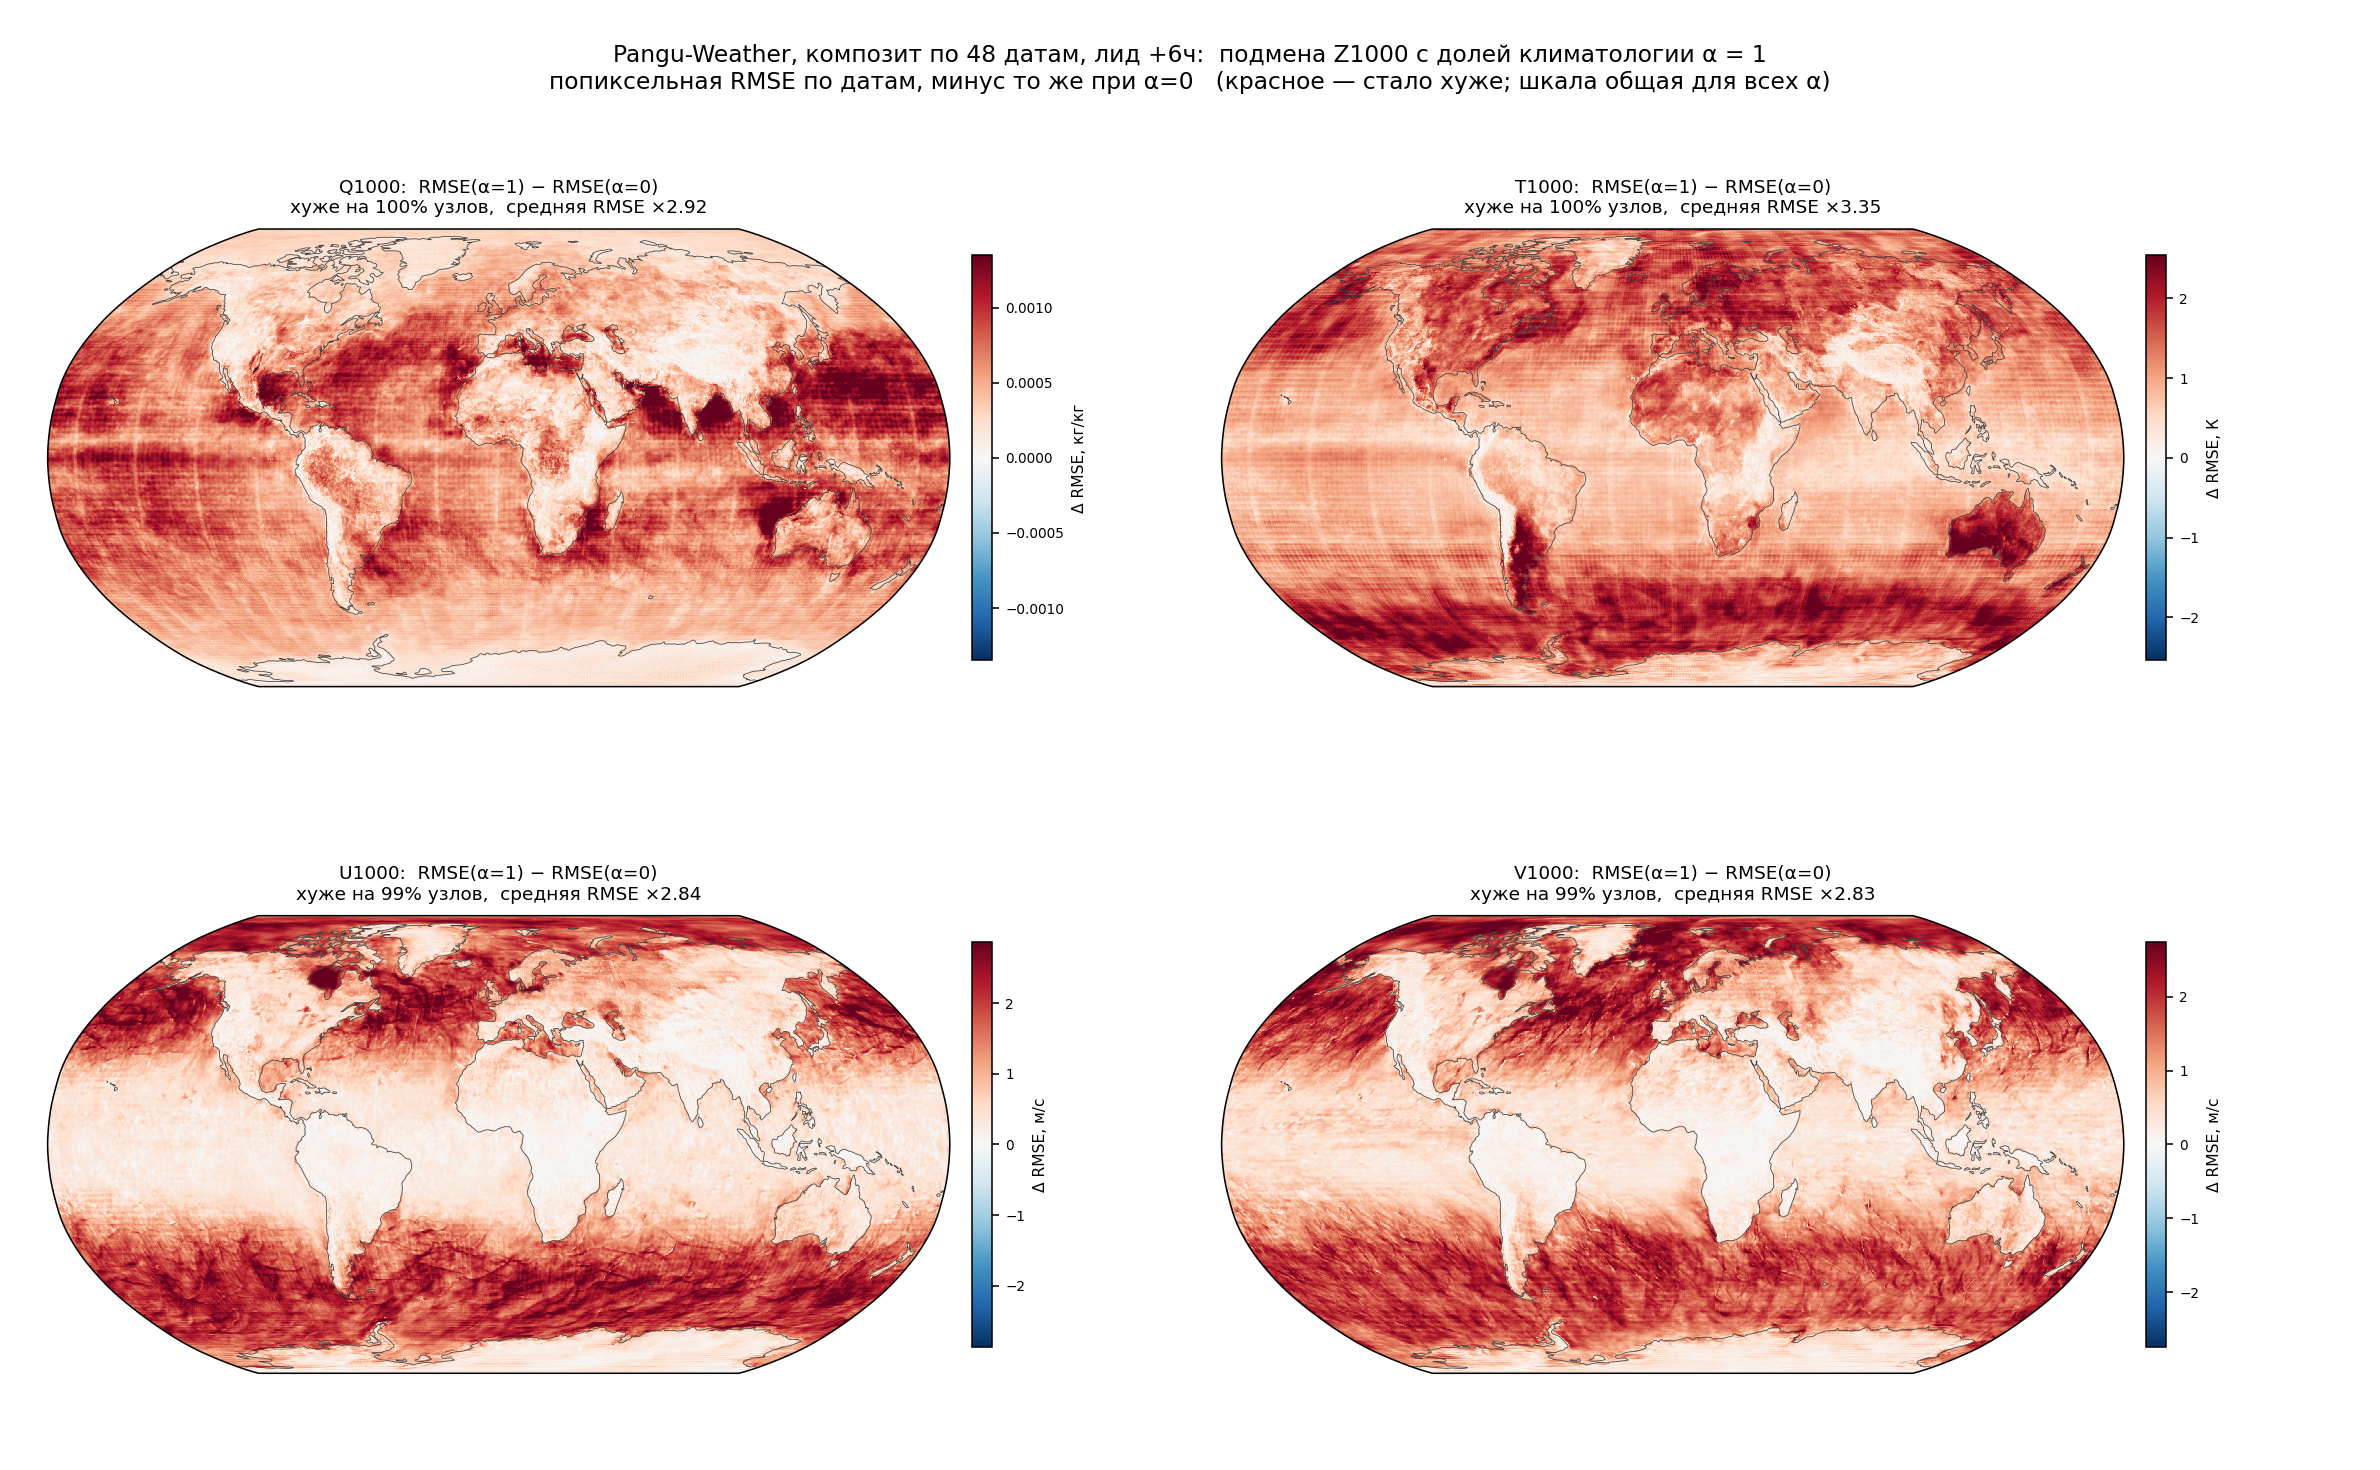
\includegraphics[width=\linewidth,trim=8.10in 5.55in 0.20in 1.58in,clip]{../../figures/bias_maps/composite_bias_pangu_Z1000_lead6_alpha1_n48.png}
  \\(b) Pangu-Weather, +6 h: $3.35\times$
\end{minipage}

\begin{minipage}[t]{0.485\linewidth}
  \centering
  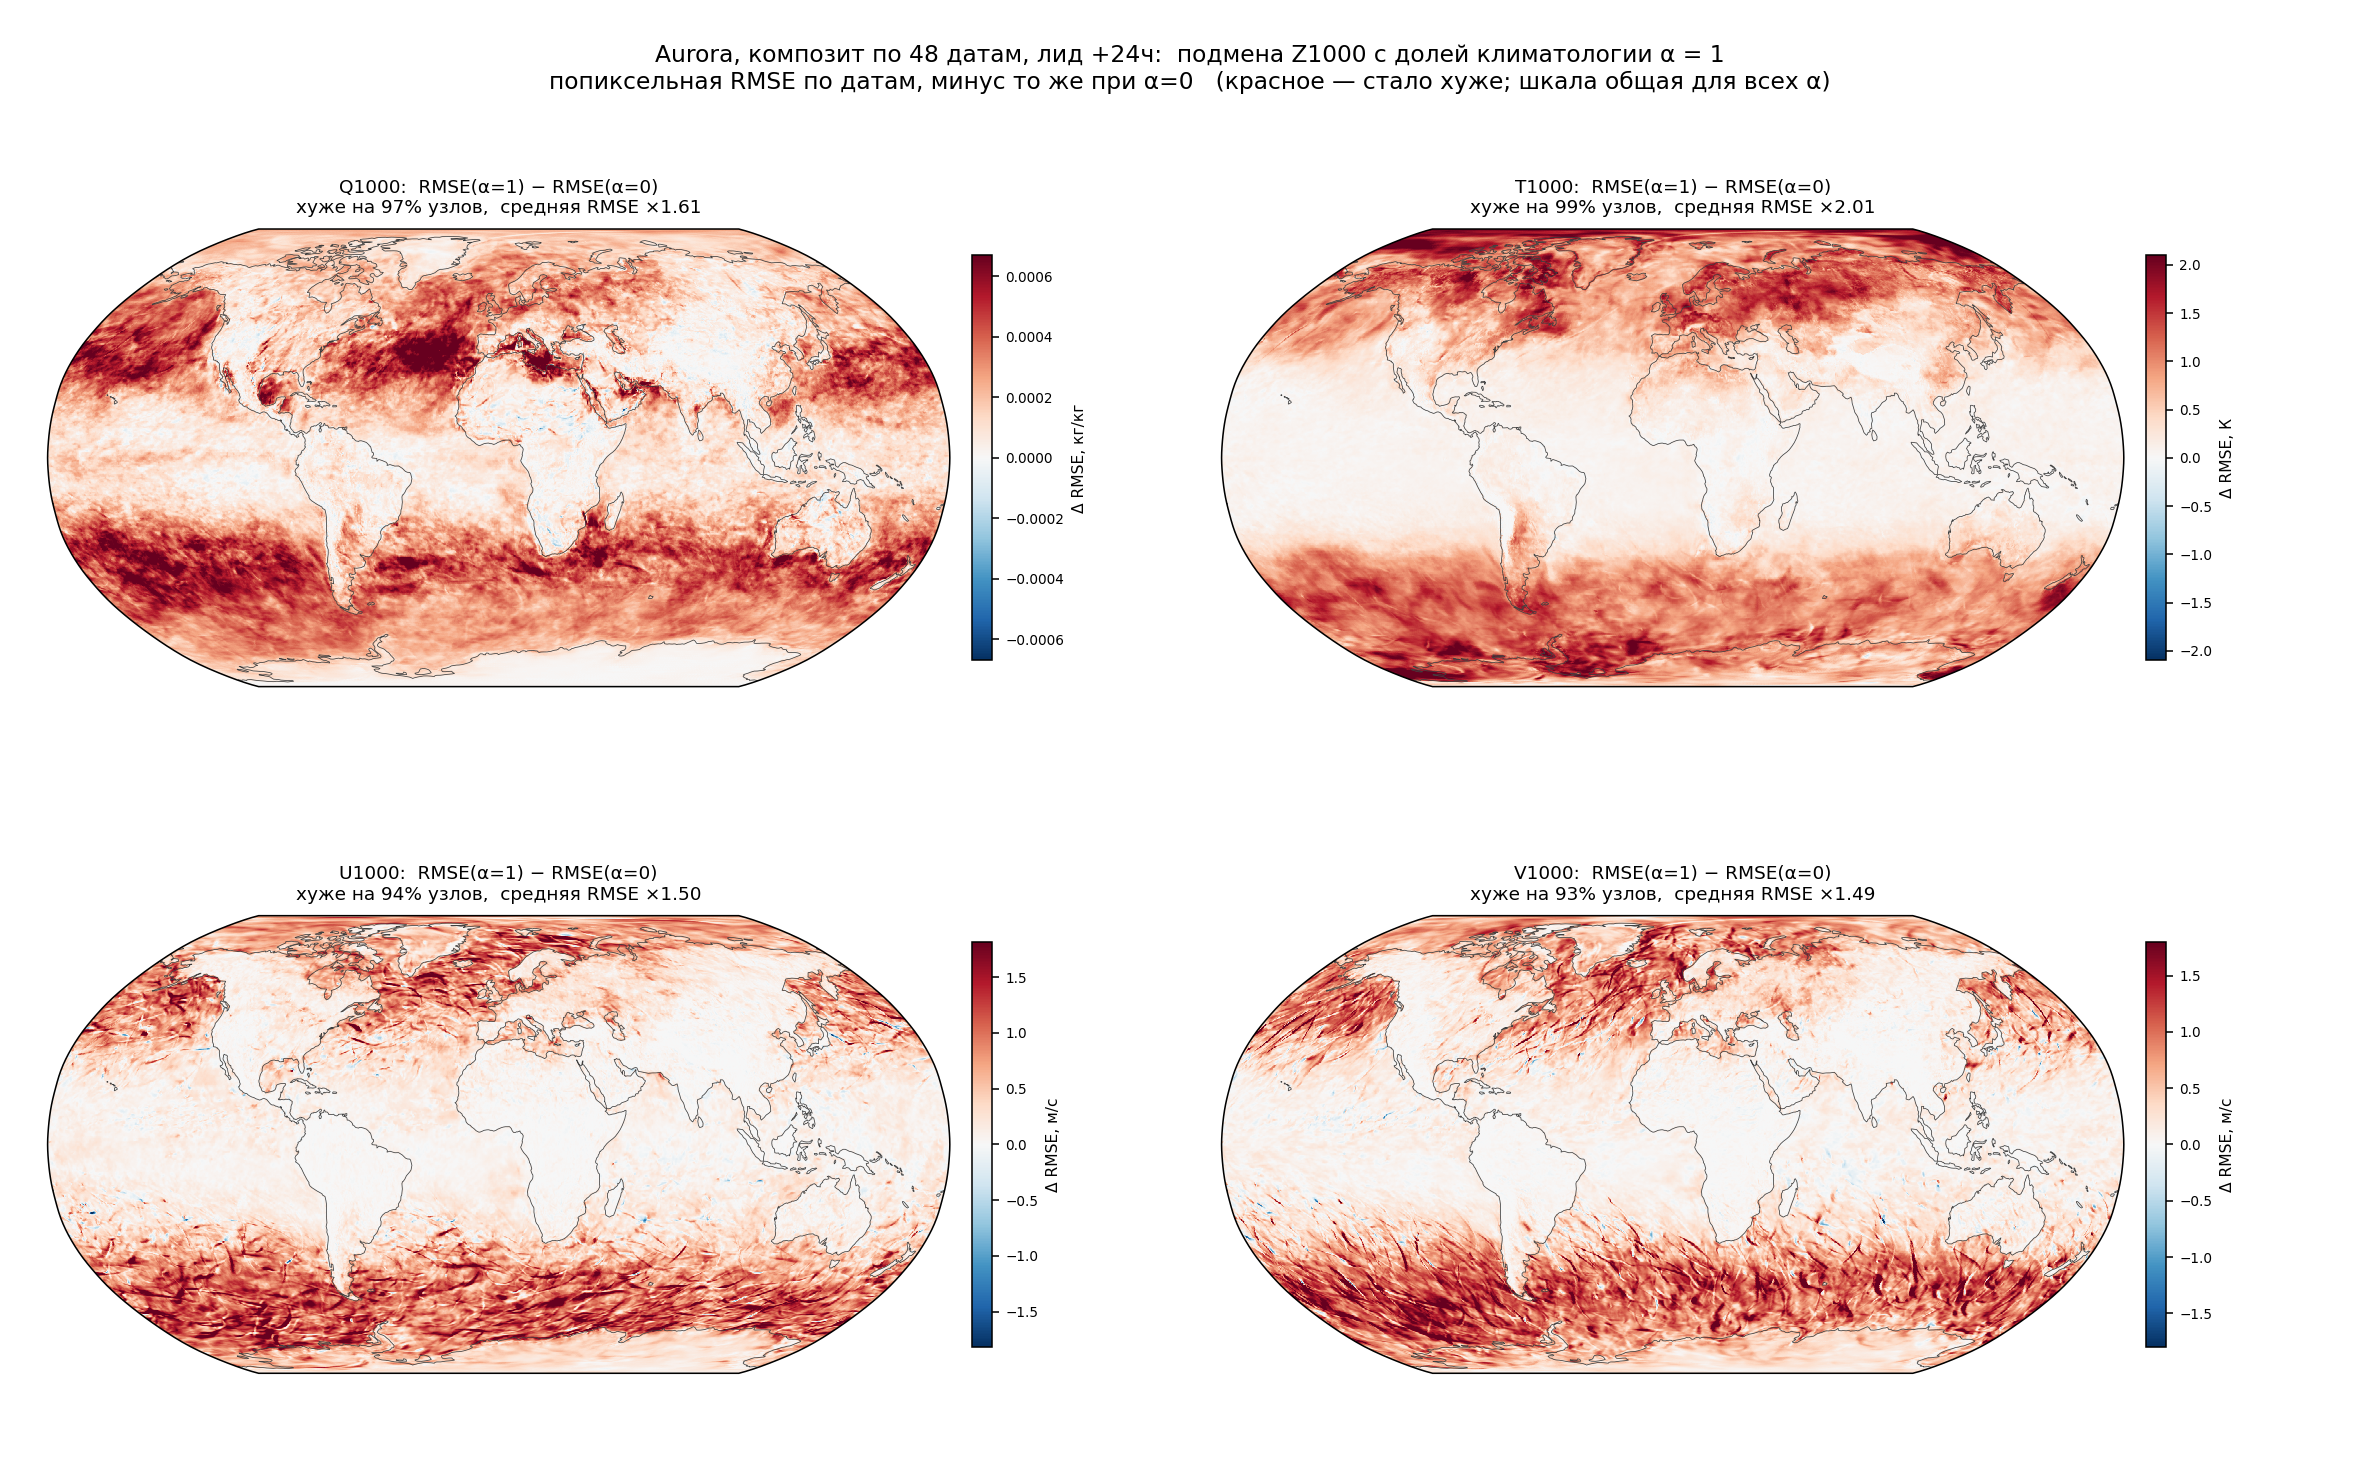
\includegraphics[width=\linewidth,trim=8.10in 5.55in 0.20in 1.58in,clip]{../../figures/bias_maps/composite_bias_Z1000_lead24_alpha1_n48.png}
  \\(c) Aurora, +24 h: $2.01\times$
\end{minipage}\hfill
\begin{minipage}[t]{0.485\linewidth}
  \centering
  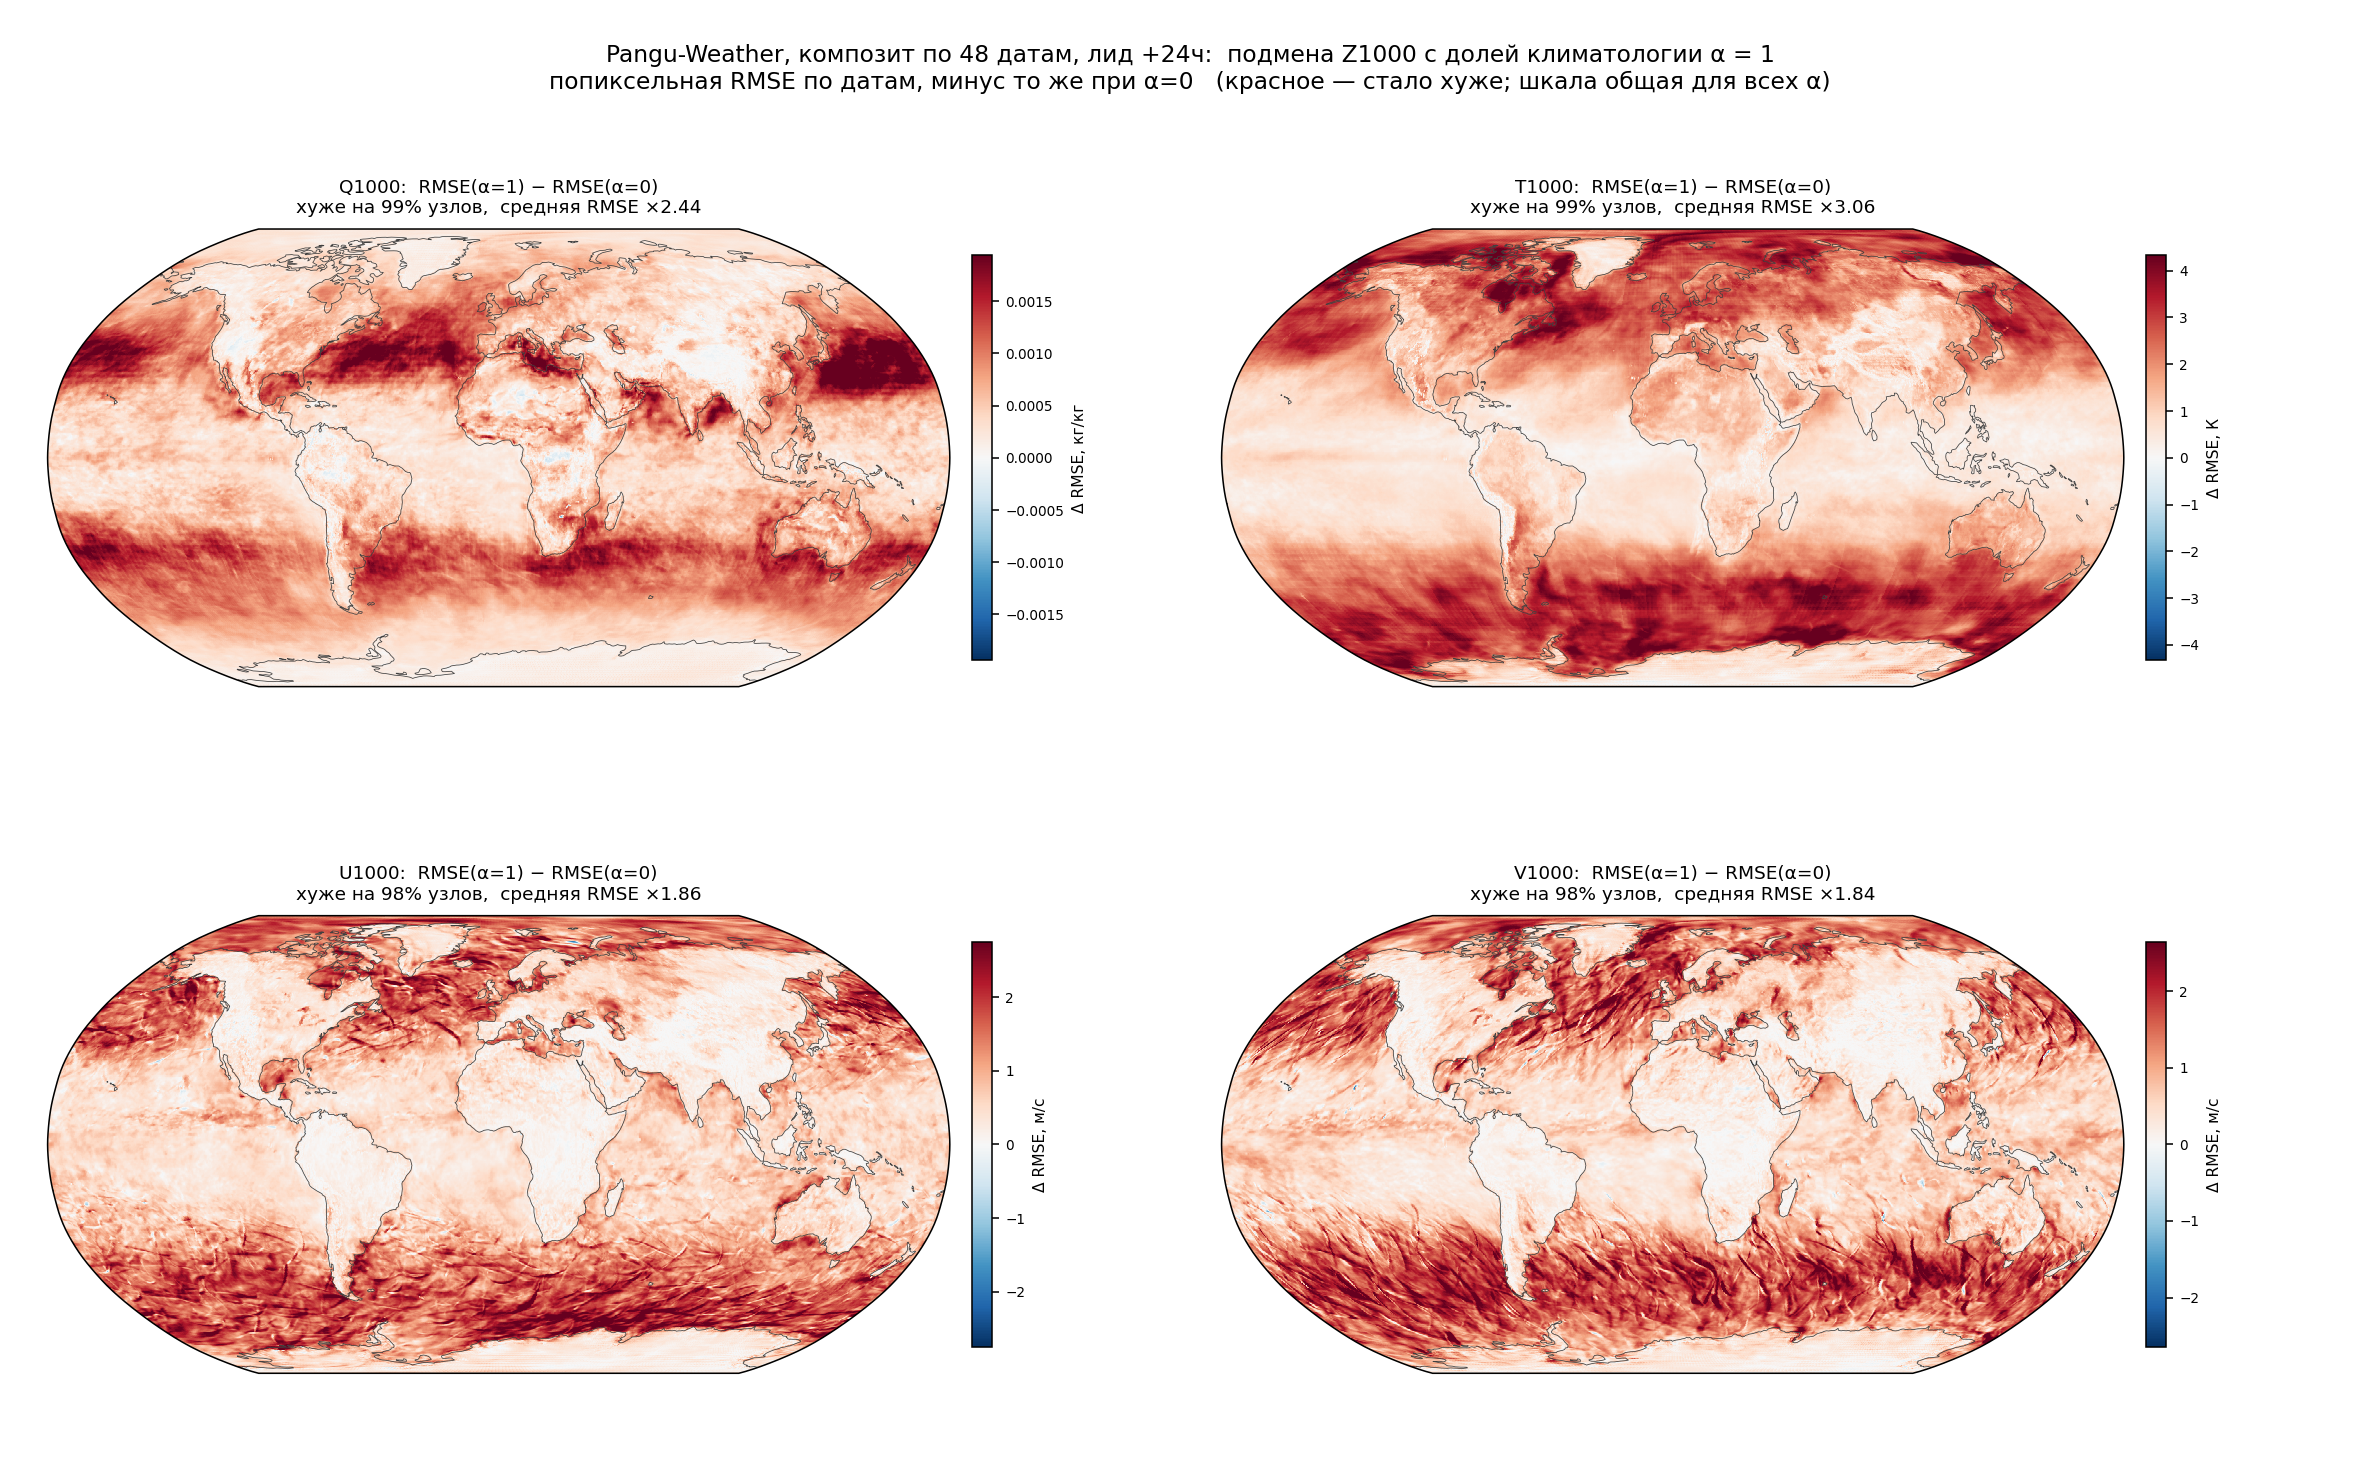
\includegraphics[width=\linewidth,trim=8.10in 5.55in 0.20in 1.58in,clip]{../../figures/bias_maps/composite_bias_pangu_Z1000_lead24_alpha1_n48.png}
  \\(d) Pangu-Weather, +24 h: $3.06\times$
\end{minipage}
\caption{$T1000$ change in per-grid-cell temporal RMSE after full $Z1000$ replacement ($\alpha=1$). Red marks larger error than the baseline. Each panel keeps its source color scale; the labels report the global mean ratio of per-cell RMSE.}
\label{fig:bias}
\end{figure}

\section{Discussion}

Mass--wind coupling and the relation between geopotential thickness and lower-tropospheric temperature make the main patterns physically plausible. The intervention still identifies dependence inside a fitted network only. Replacing a complete field with climatology is a large, partly out-of-distribution change, and single-time spatial correlations mix geography, season, and dynamics.

The evaluation covers 48 dates from one year, two short leads, and three pressure levels. It has no ensembles or date-block bootstrap intervals. The raw arrays live in an external cluster store that was unavailable during paper assembly, so we checked the numbers against committed figures, captions, and analysis code without recomputing them. Operational evaluation needs uncertainty intervals, event stratification, longer leads, and true issue-time data.

\paragraph{Climate relevance and risks.} Forecast developers can use the audit to find brittle channel dependence before a model enters an early-warning or climate-service pipeline. The audit does not improve forecast skill, quantify anthropogenic climate change, or validate a decision rule. It should sit beside standard skill, calibration, and expert review. The next experiment should repeat the paired intervention across events and forecast ranges, with date-block uncertainty intervals computed from issue-time data.

\clearpage
\bibliographystyle{unsrt}
\bibliography{references}

\clearpage
\appendix
\section{Full-resolution visual evidence}
\label{app:figures}

\begin{figure}[ht]
\centering
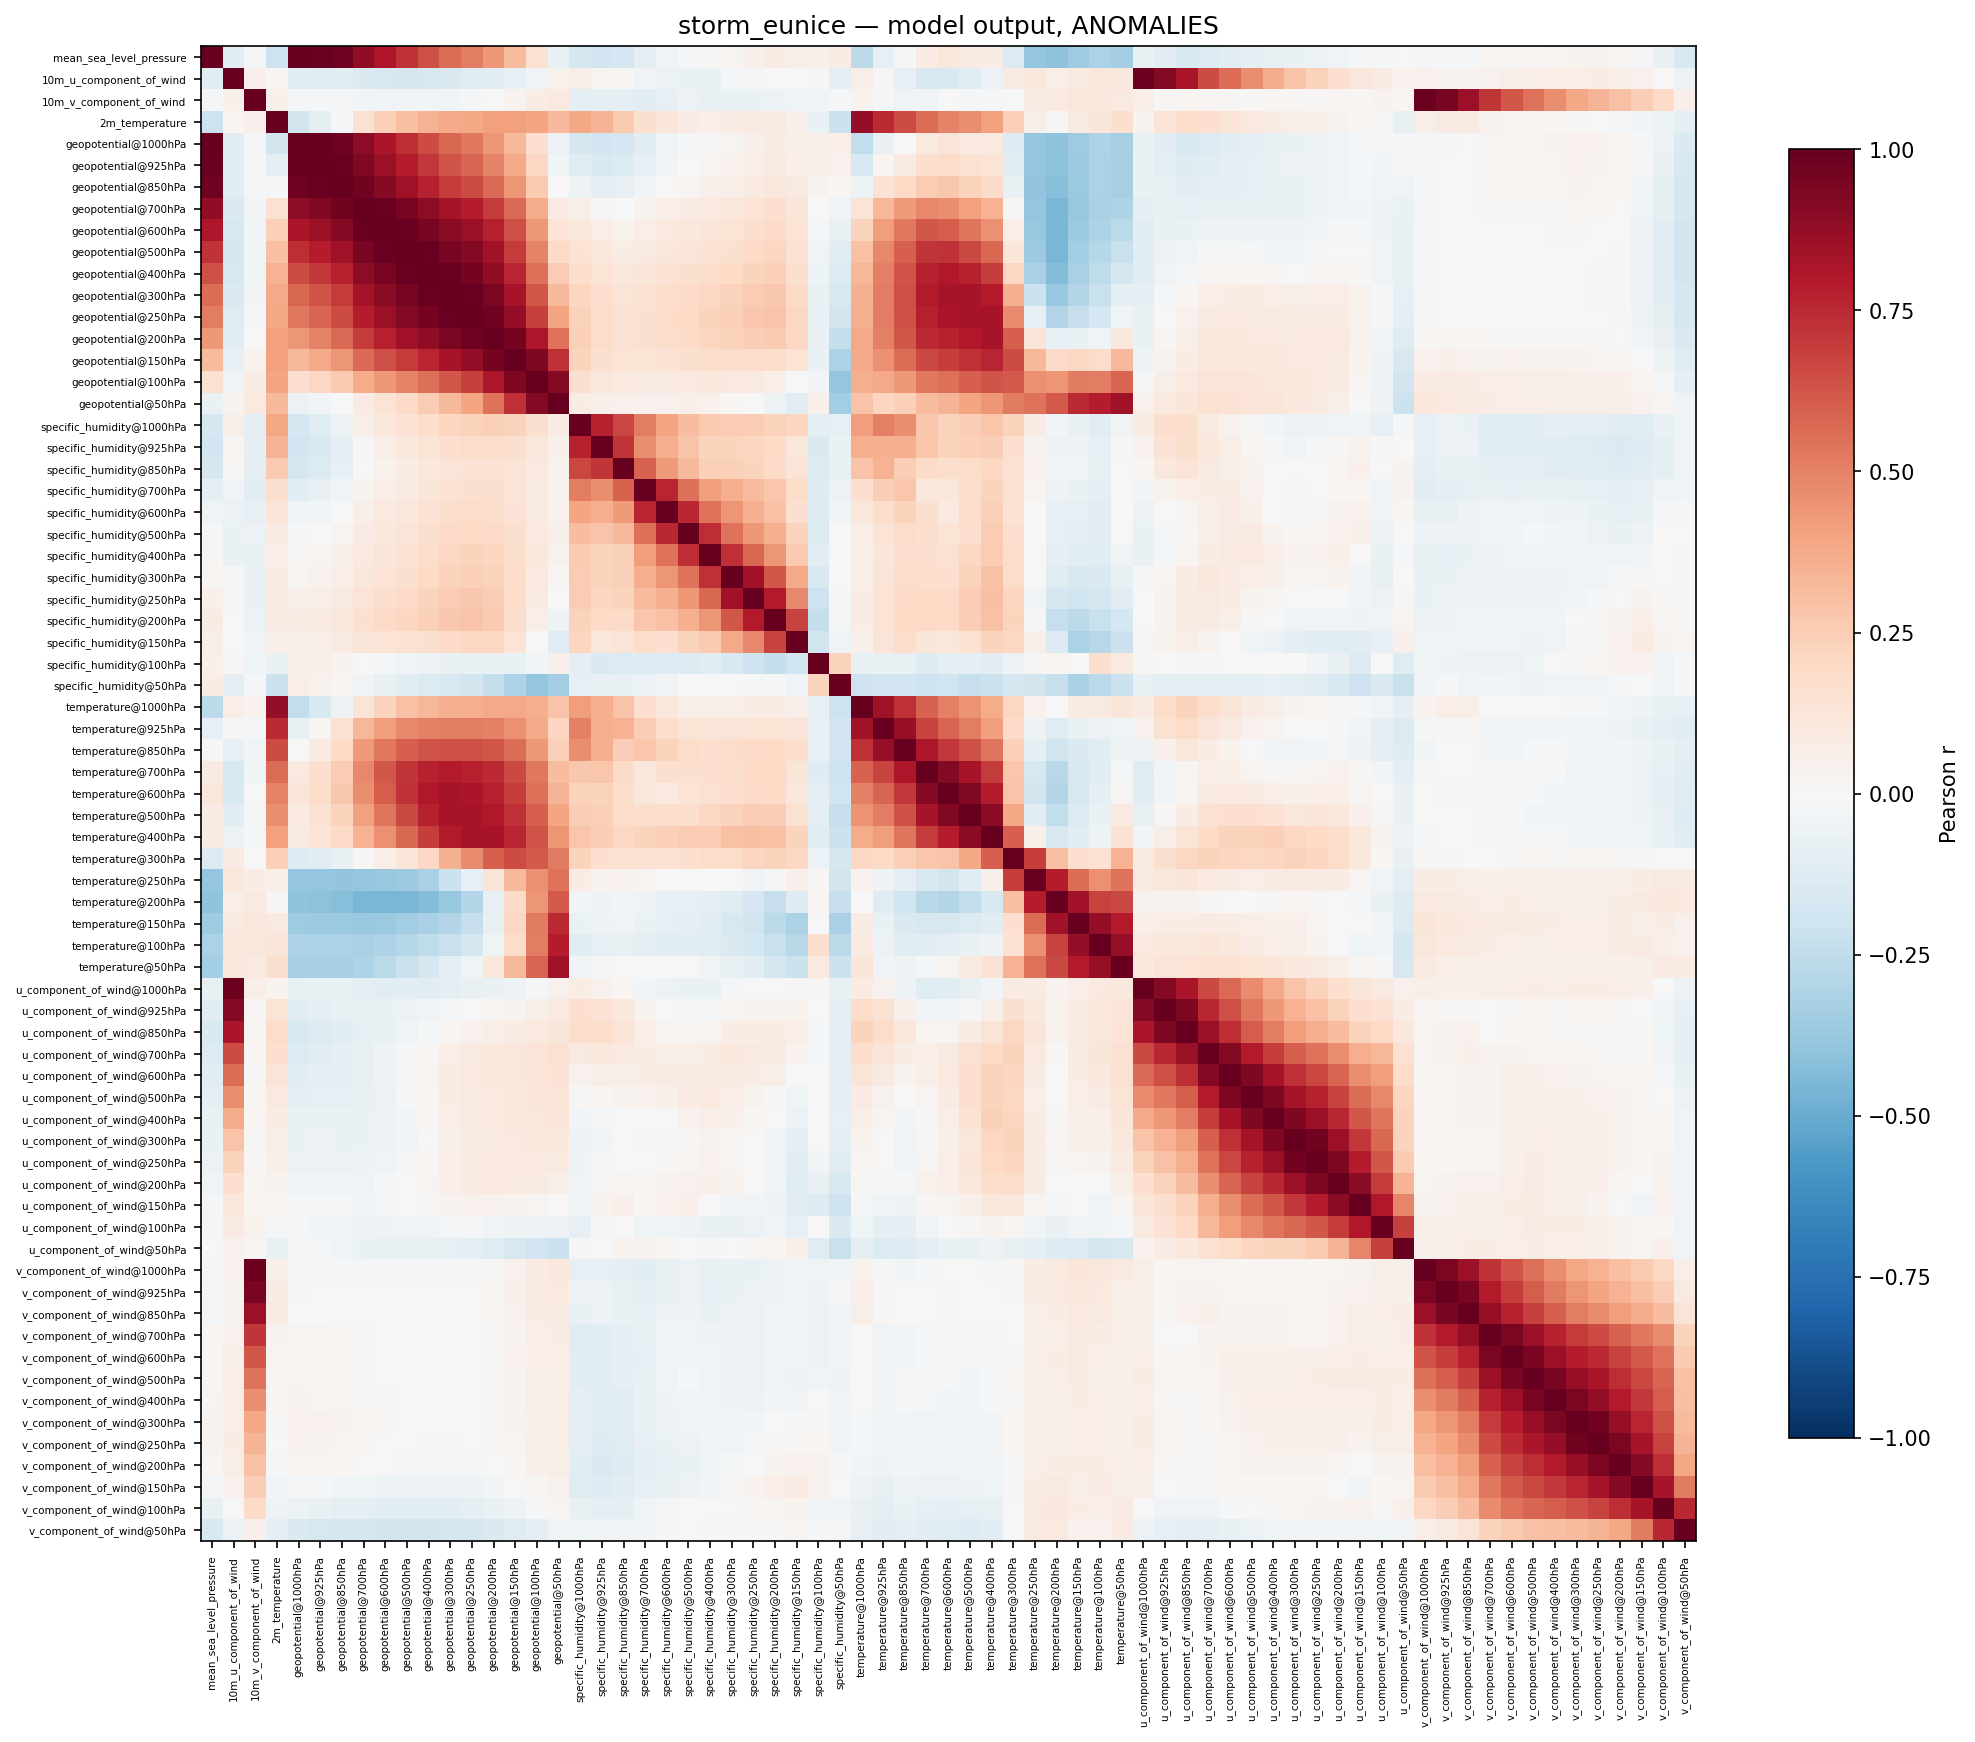
\includegraphics[width=\linewidth]{../../figures/model_comparison/storm_eunice_corr_model_anomaly.png}
\caption{Representative 69-channel output-anomaly correlation matrix for Pangu-Weather on Storm Eunice. The visible block structure is descriptive and non-directional.}
\end{figure}

\begin{figure}[p]
\centering
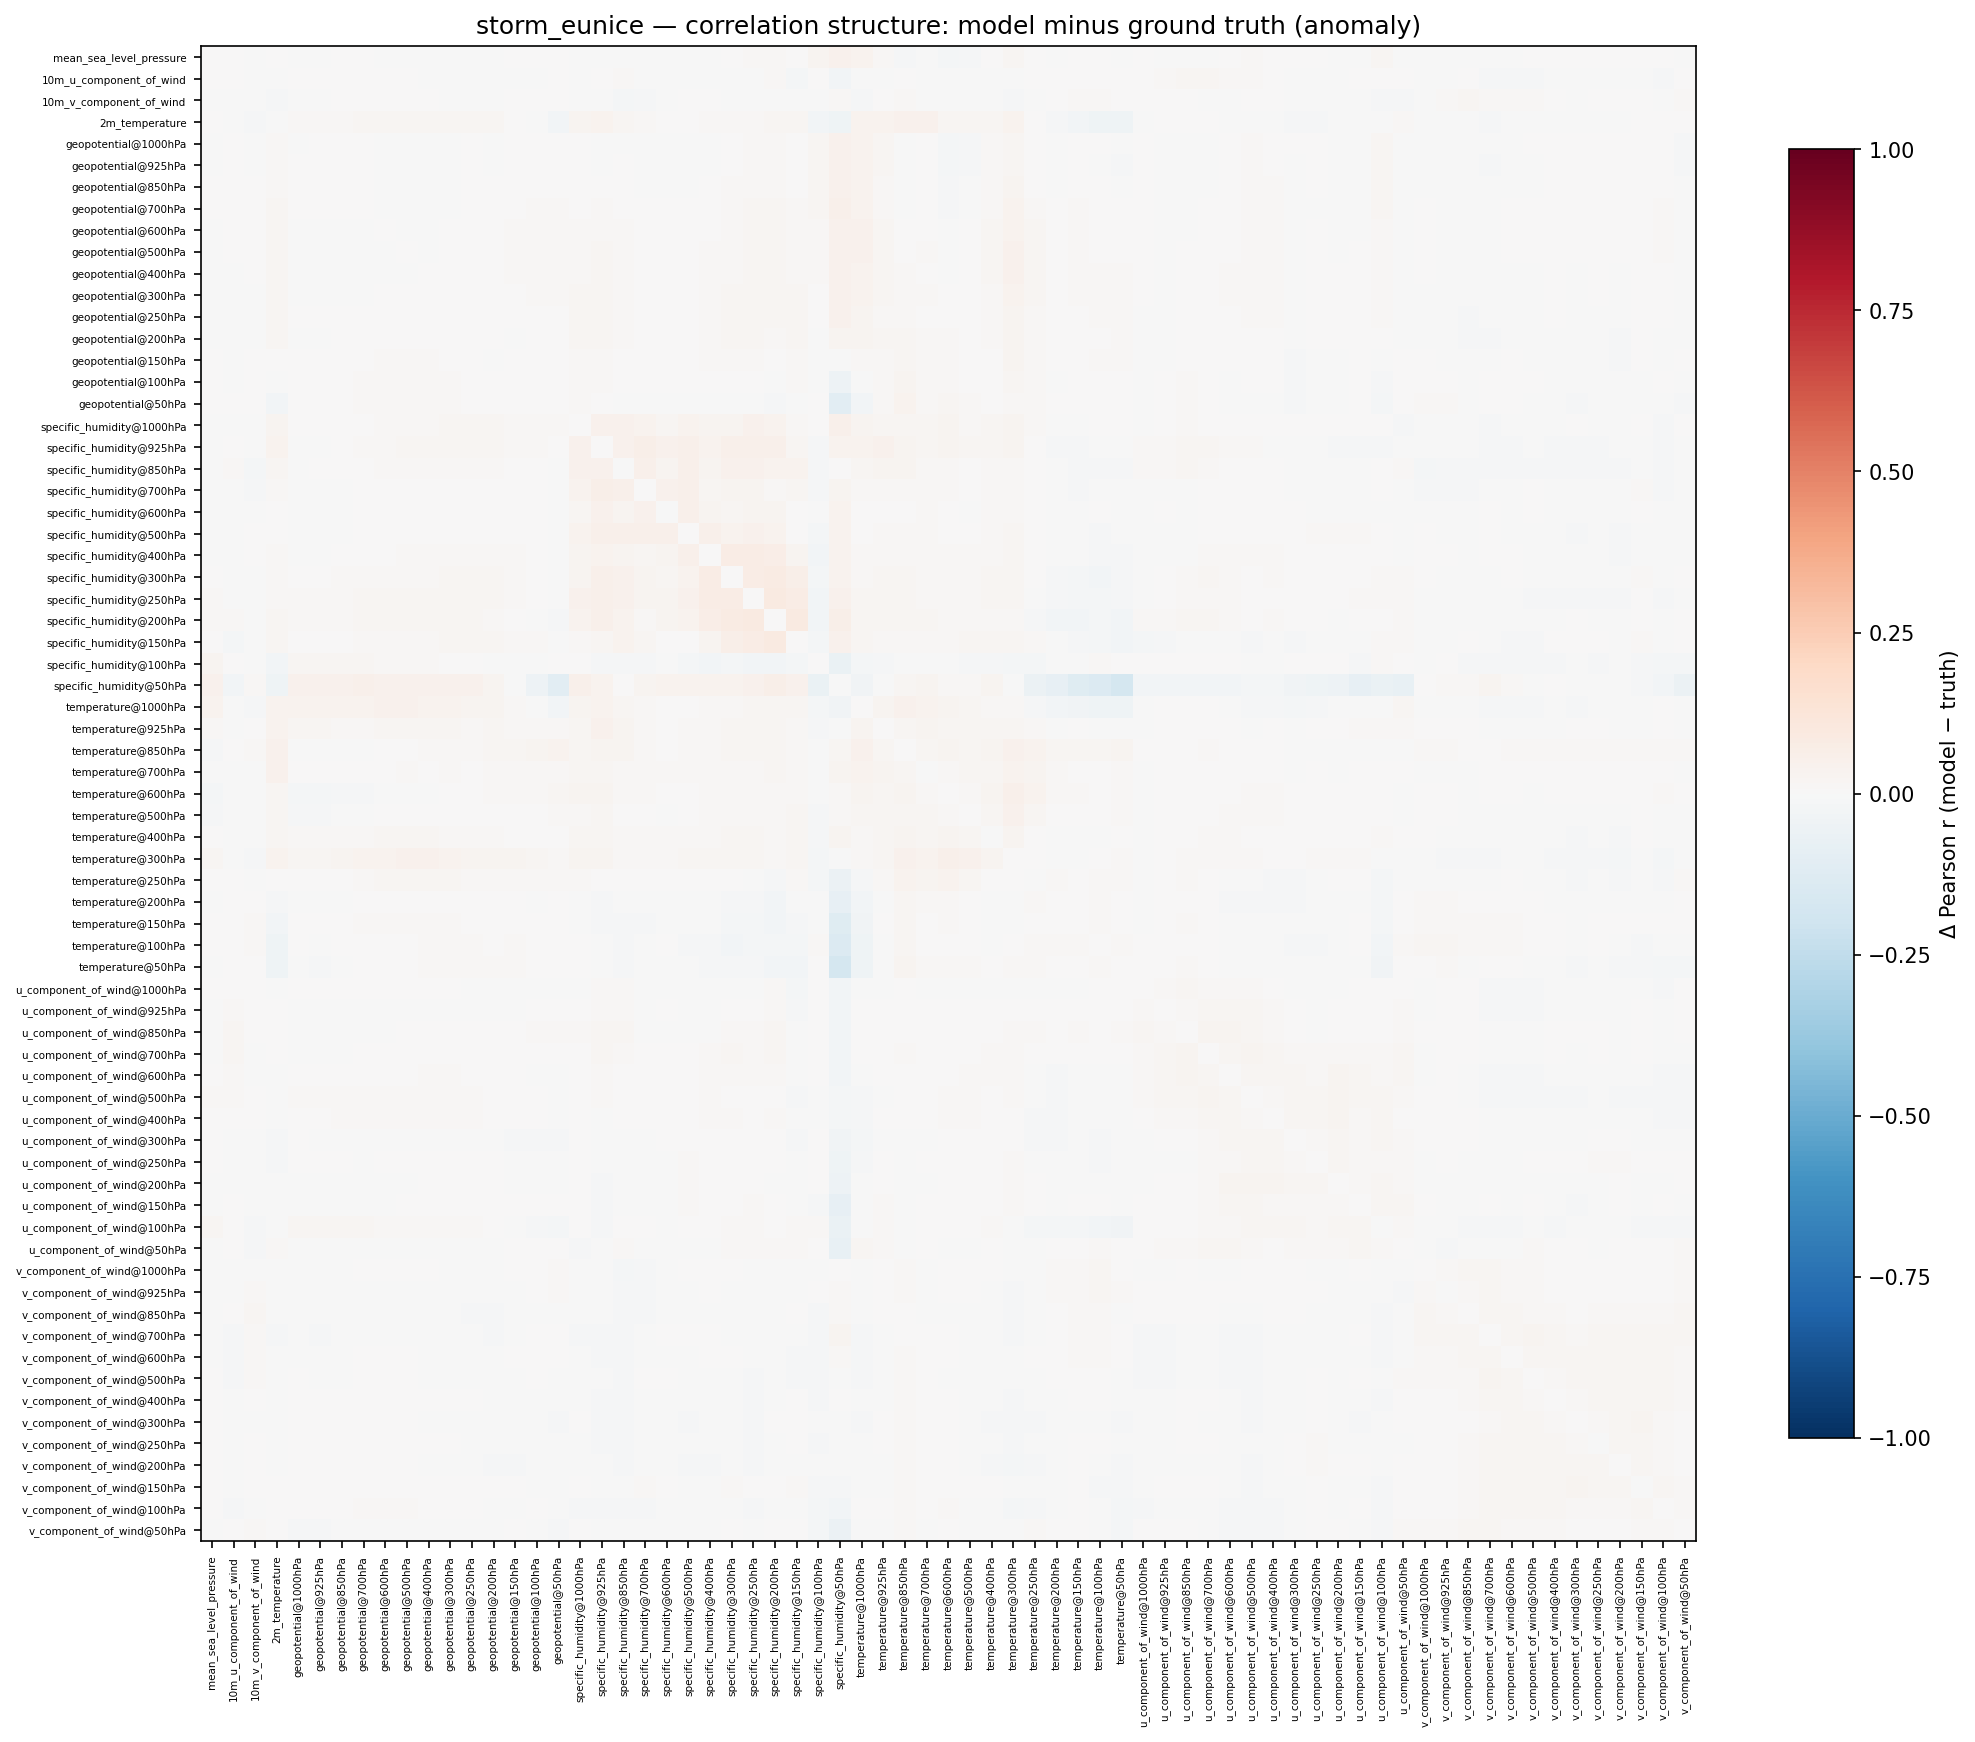
\includegraphics[width=\linewidth]{../../figures/model_comparison/storm_eunice_corr_diff_anomaly.png}
\caption{Pangu-Weather minus ERA5 anomaly-correlation structure for the same case.}
\end{figure}

\begin{figure}[p]
\centering
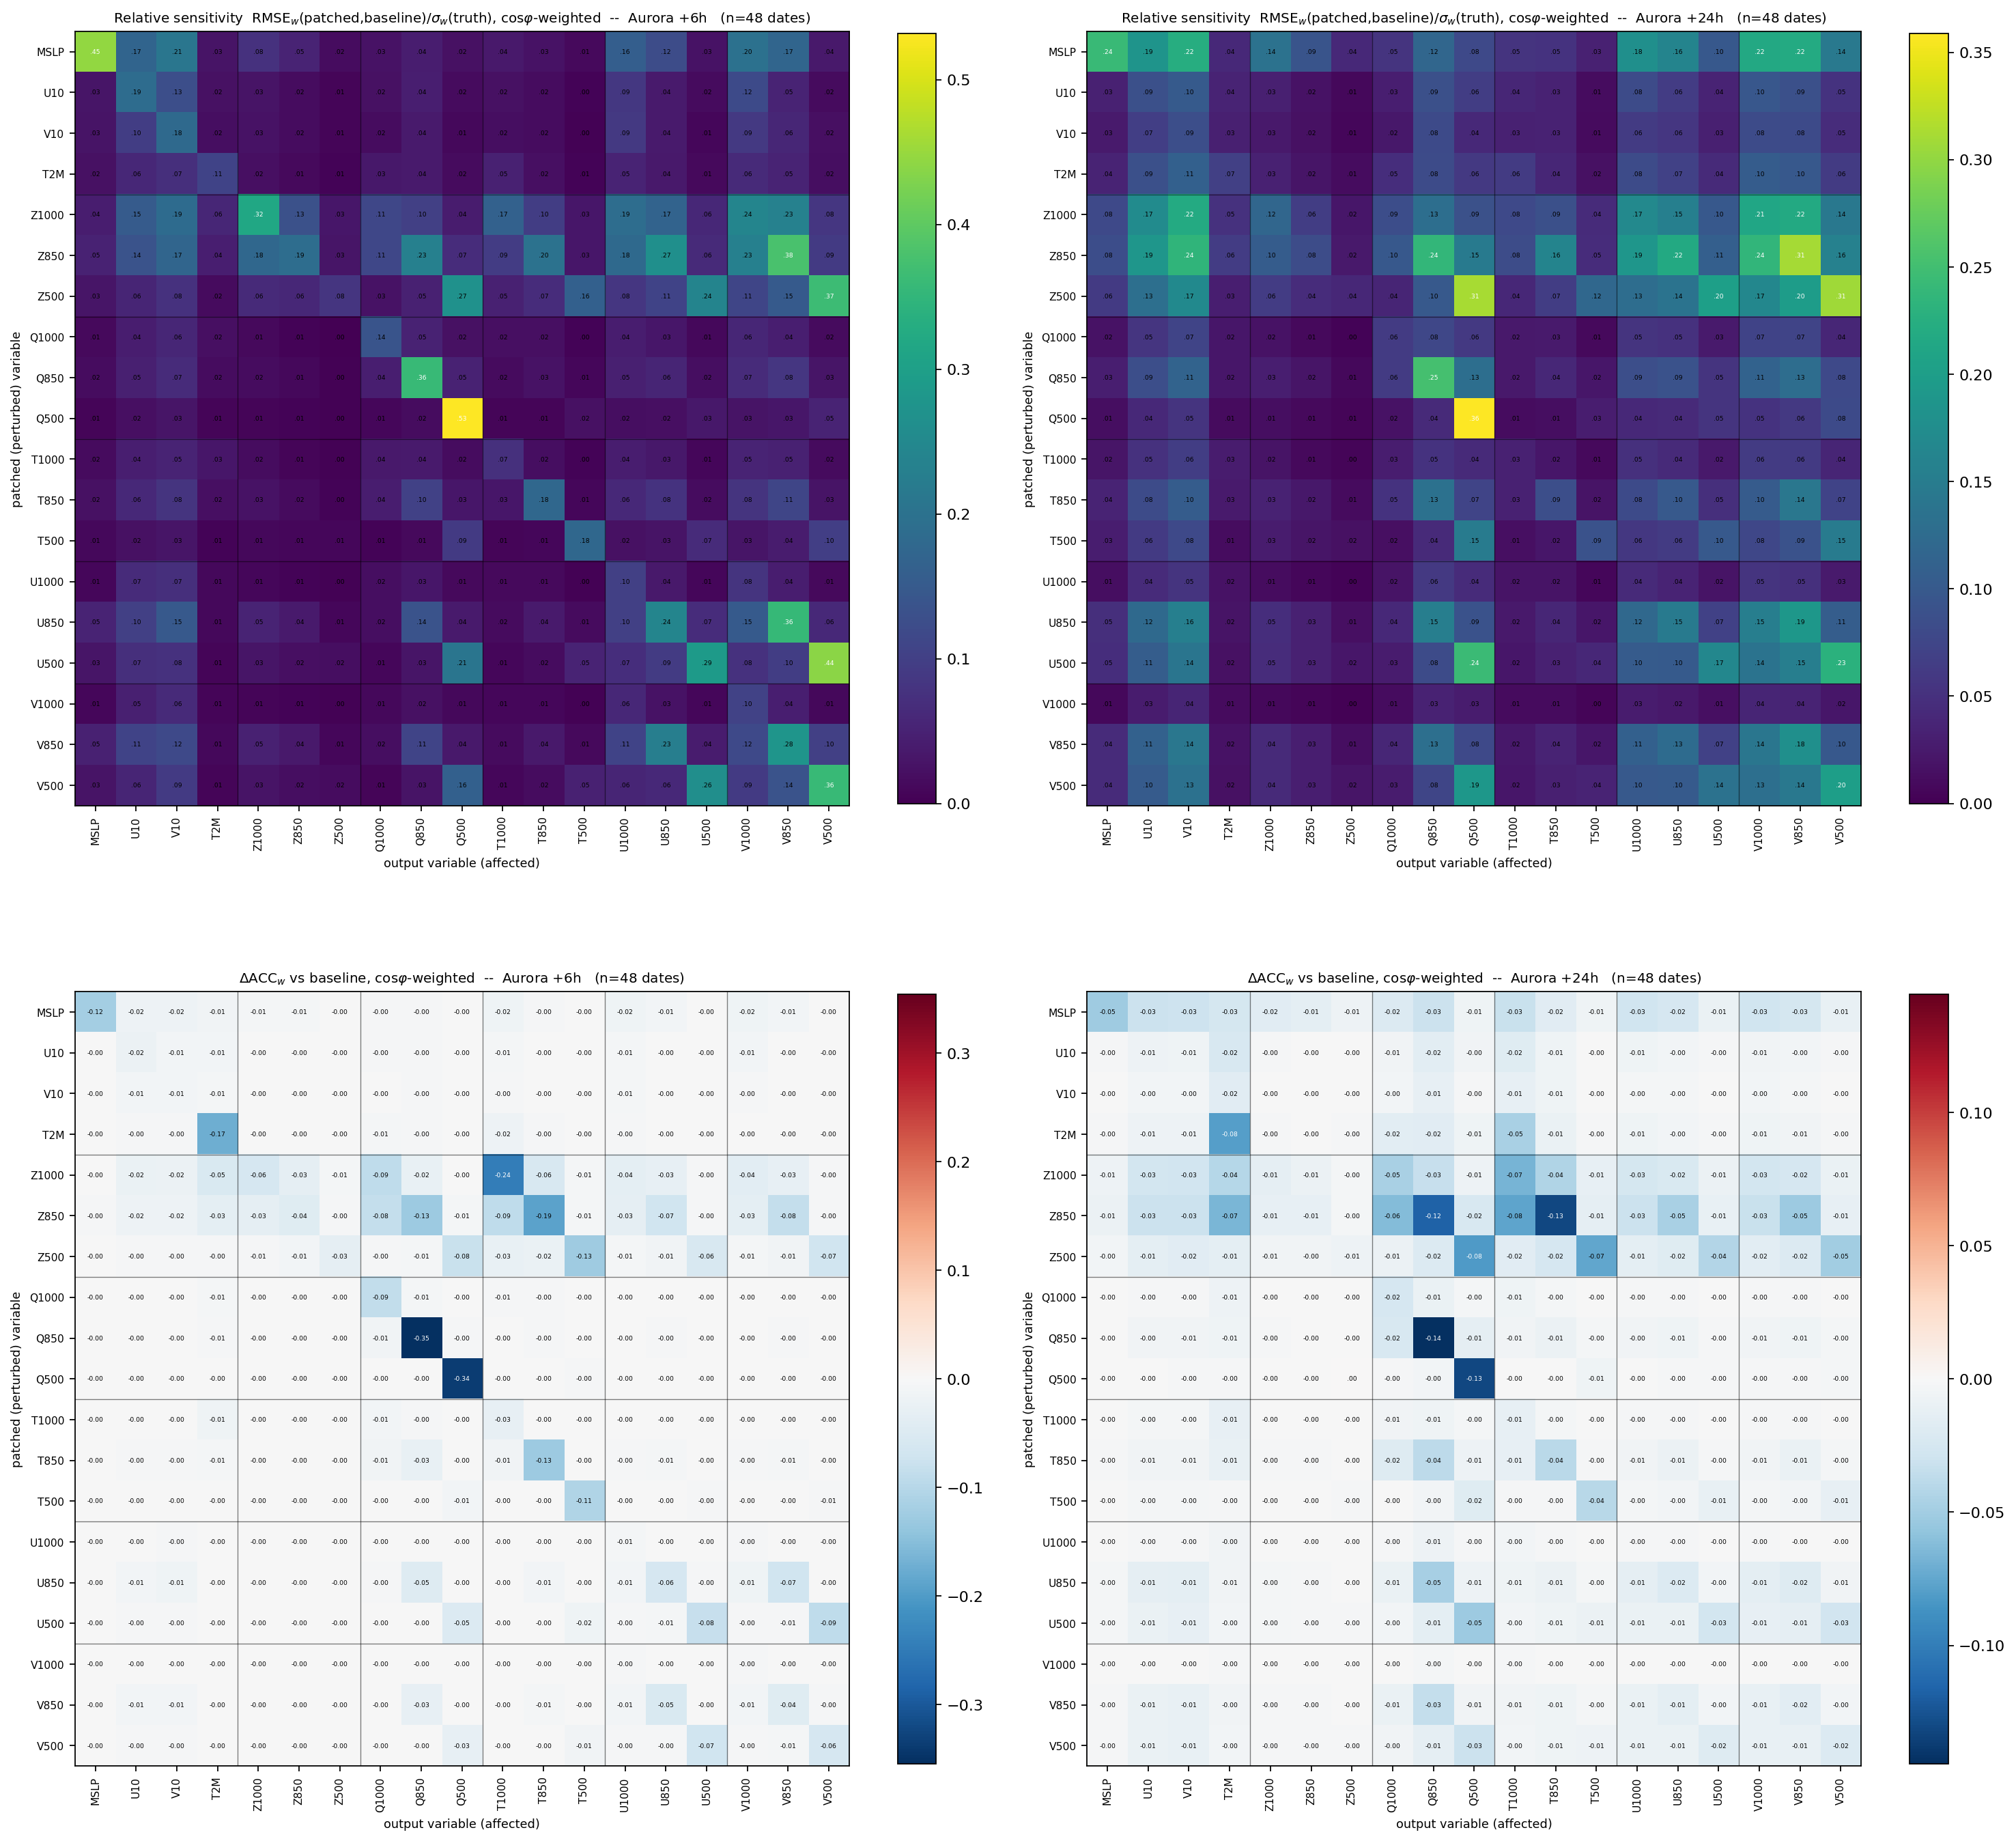
\includegraphics[width=\linewidth]{../../figures/patching_matrices/matrix_19var_aurora_n48_weighted.png}
\caption{Aurora: full area-weighted relative-sensitivity and $\Delta$ACC matrices at +6 and +24 h ($n=48$).}
\end{figure}

\begin{figure}[p]
\centering
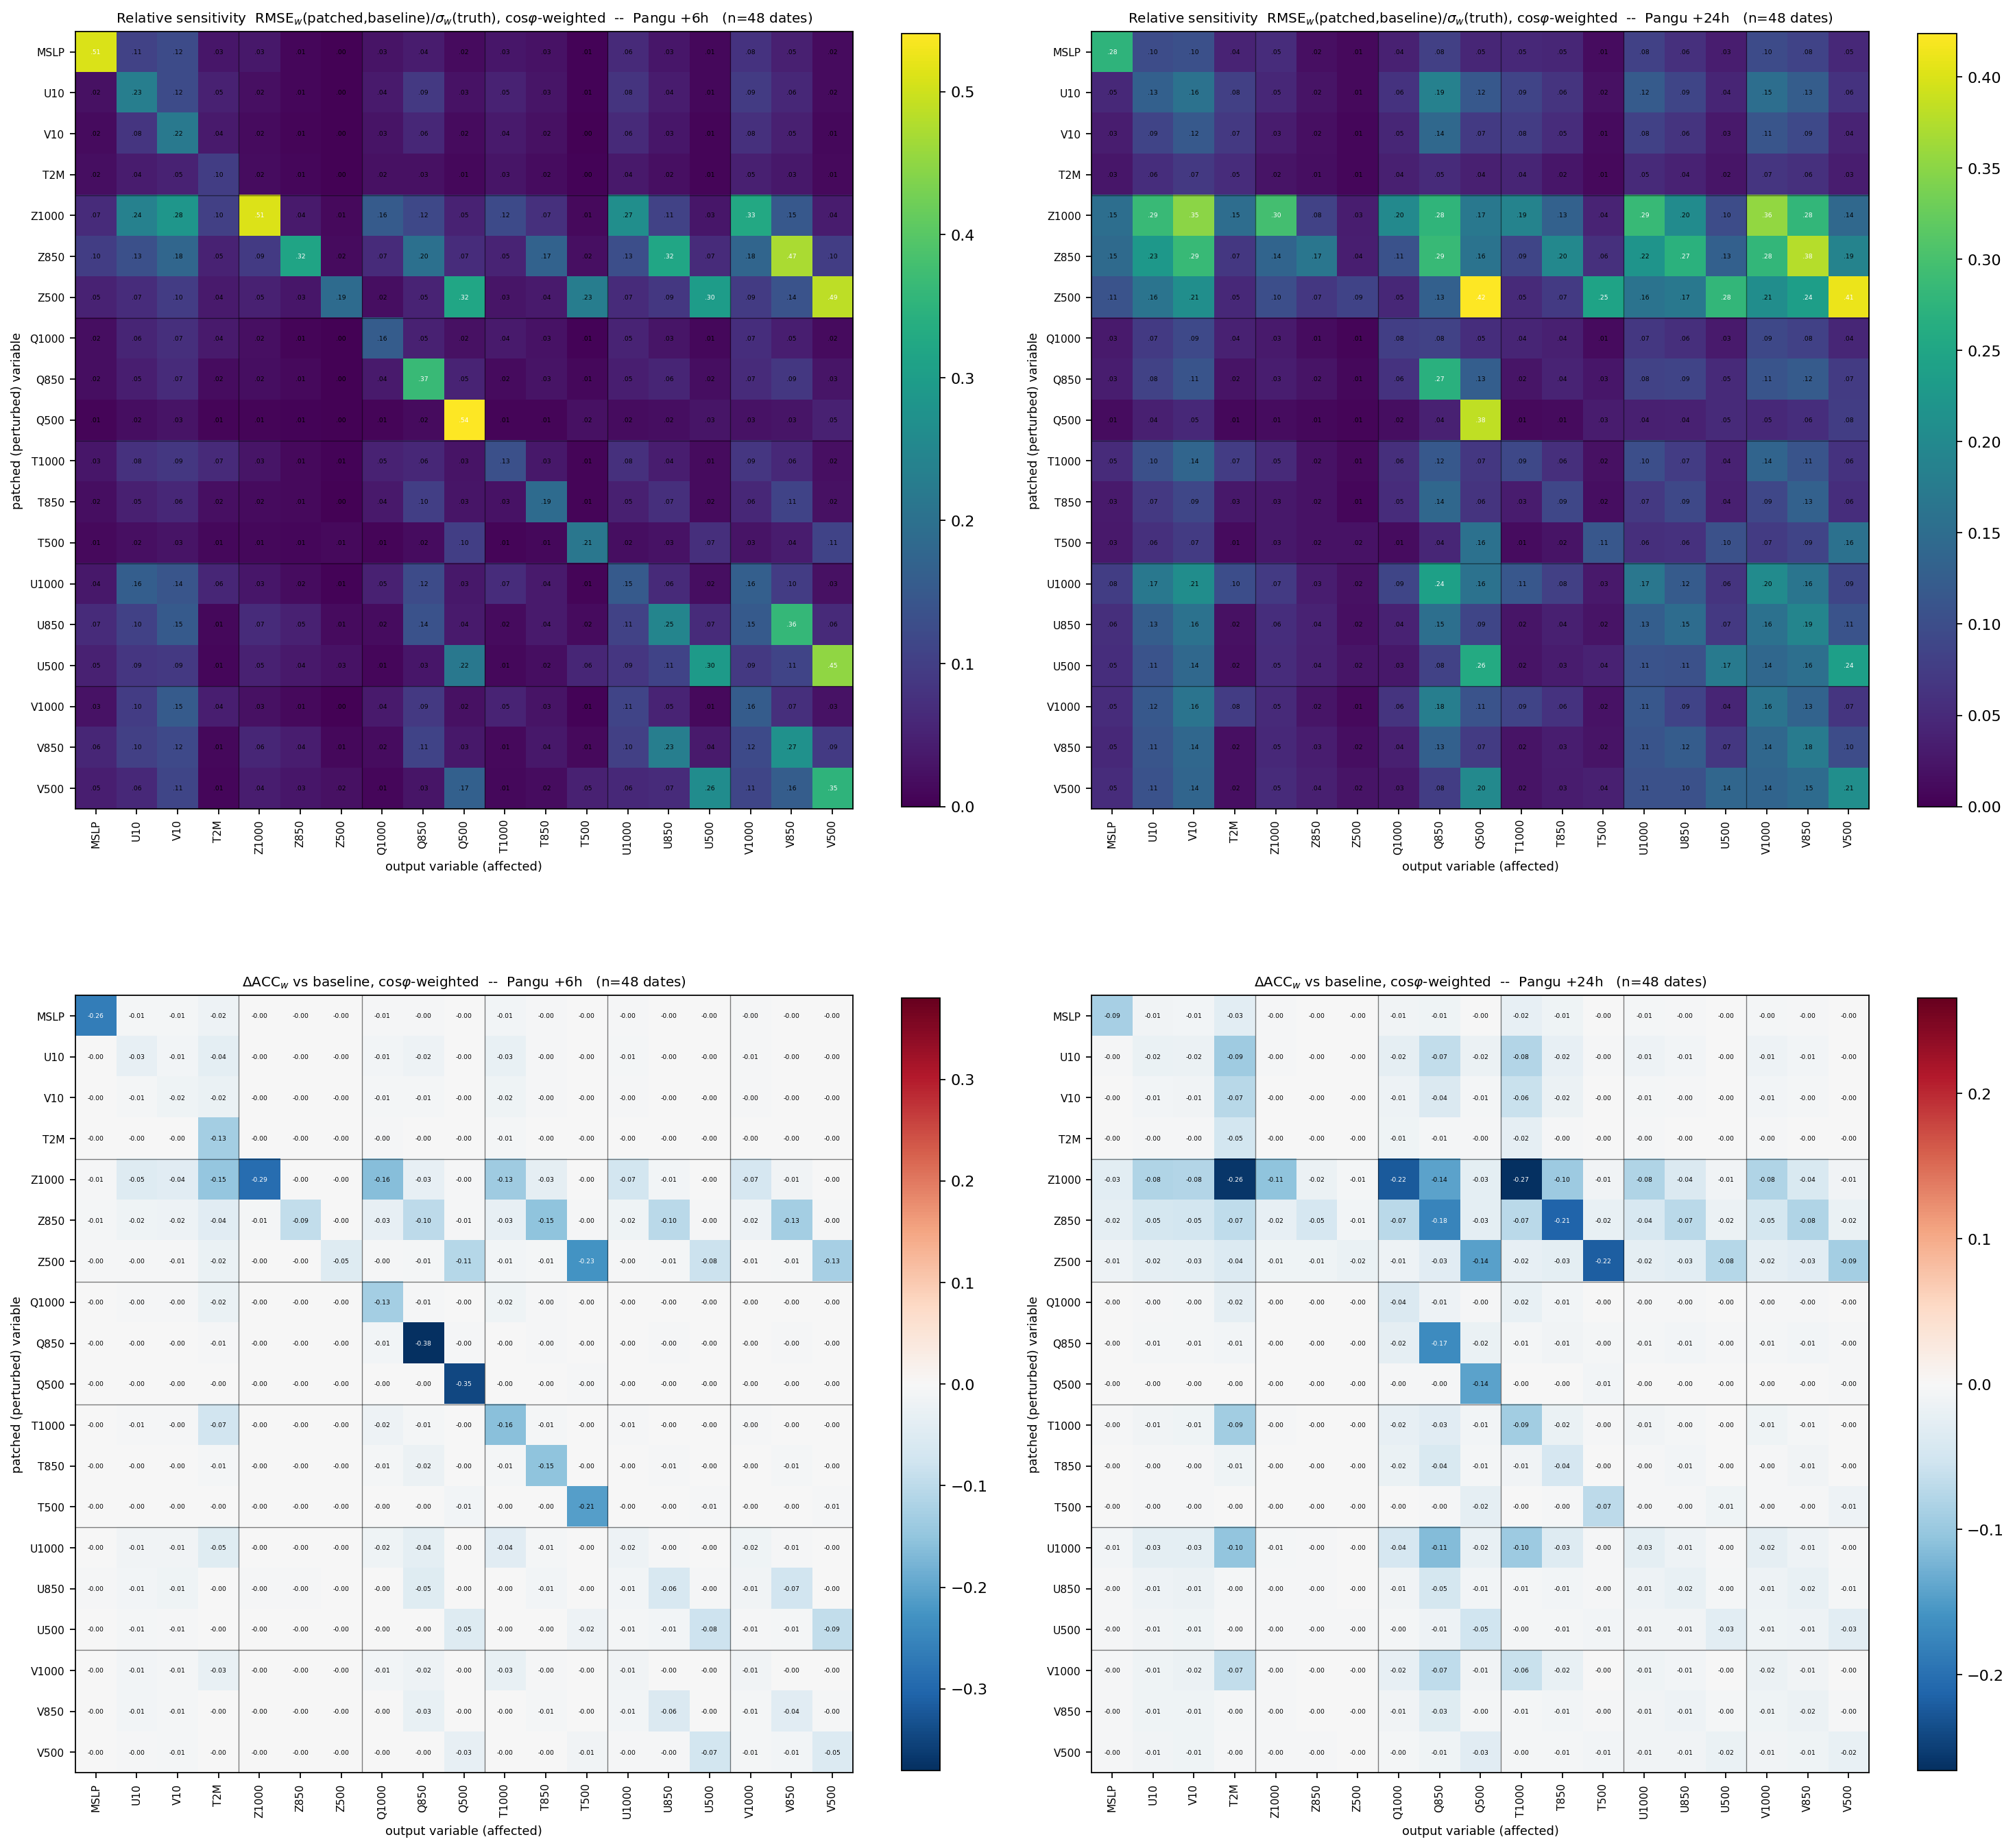
\includegraphics[width=\linewidth]{../../figures/patching_matrices/matrix_19var_pangu_n48_weighted.png}
\caption{Pangu-Weather: full area-weighted relative-sensitivity and $\Delta$ACC matrices at +6 and +24 h ($n=48$).}
\end{figure}

\begin{figure}[p]
\centering
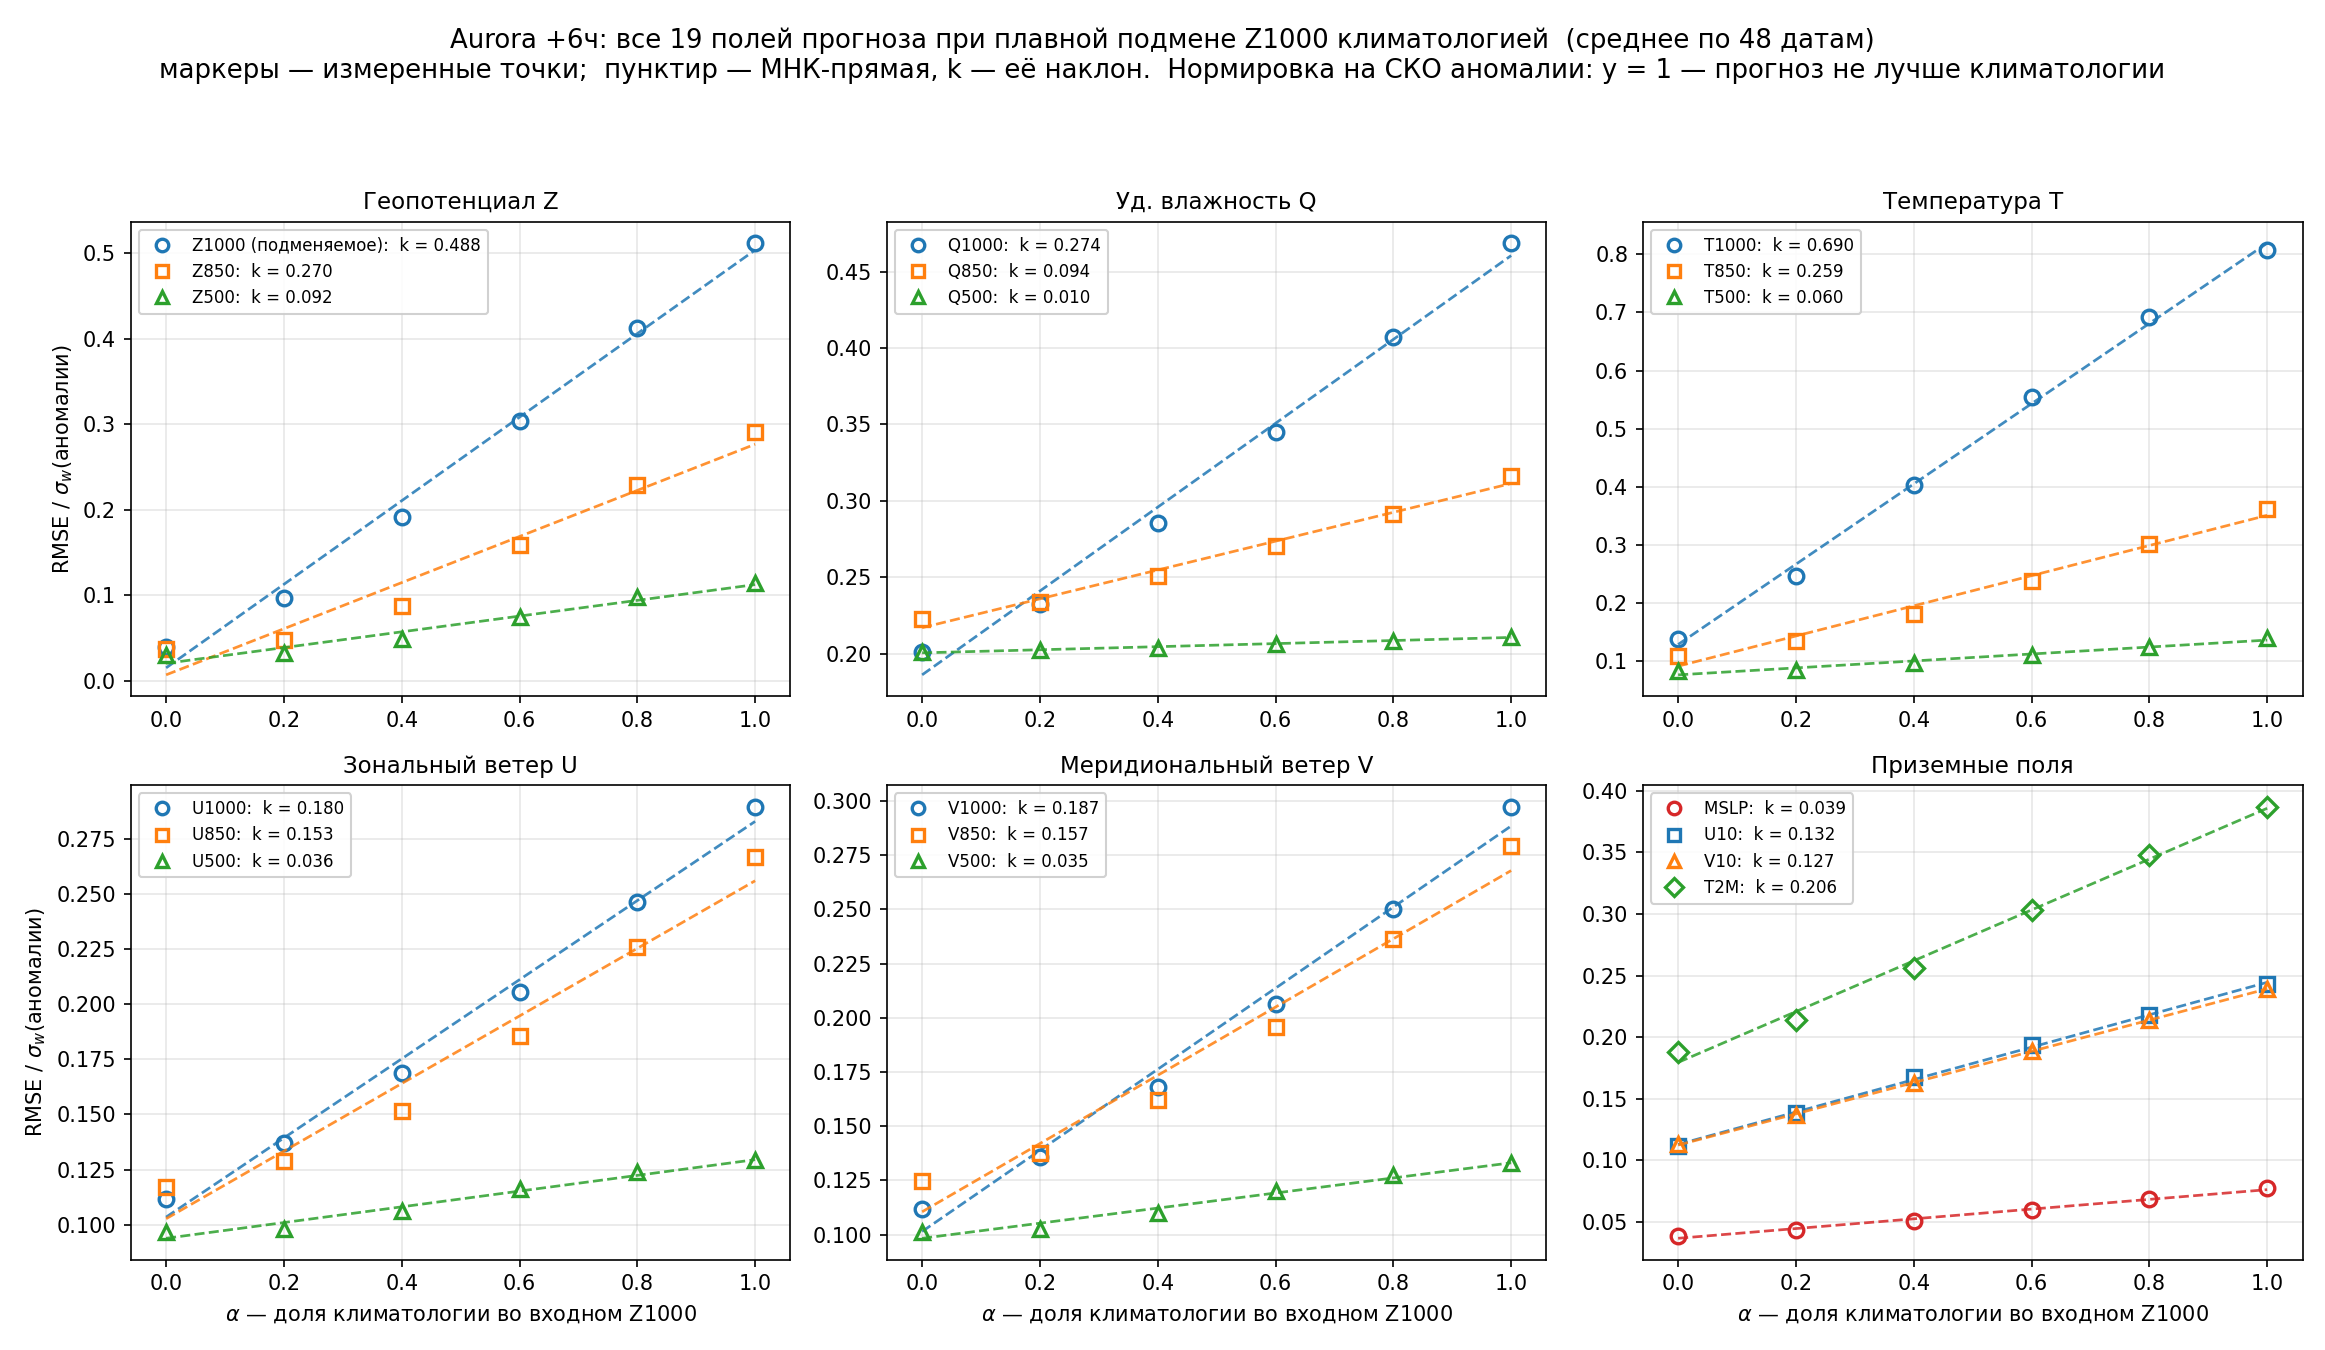
\includegraphics[width=\linewidth]{../../figures/dose_response/dose_panels_anom_Z1000_lead6_aurora_n48.png}
\caption{Aurora +6 h dose response for all 19 outputs under $Z1000$ climatology blending. The committed source panel retains its original Russian annotations.}
\end{figure}

\begin{figure}[p]
\centering
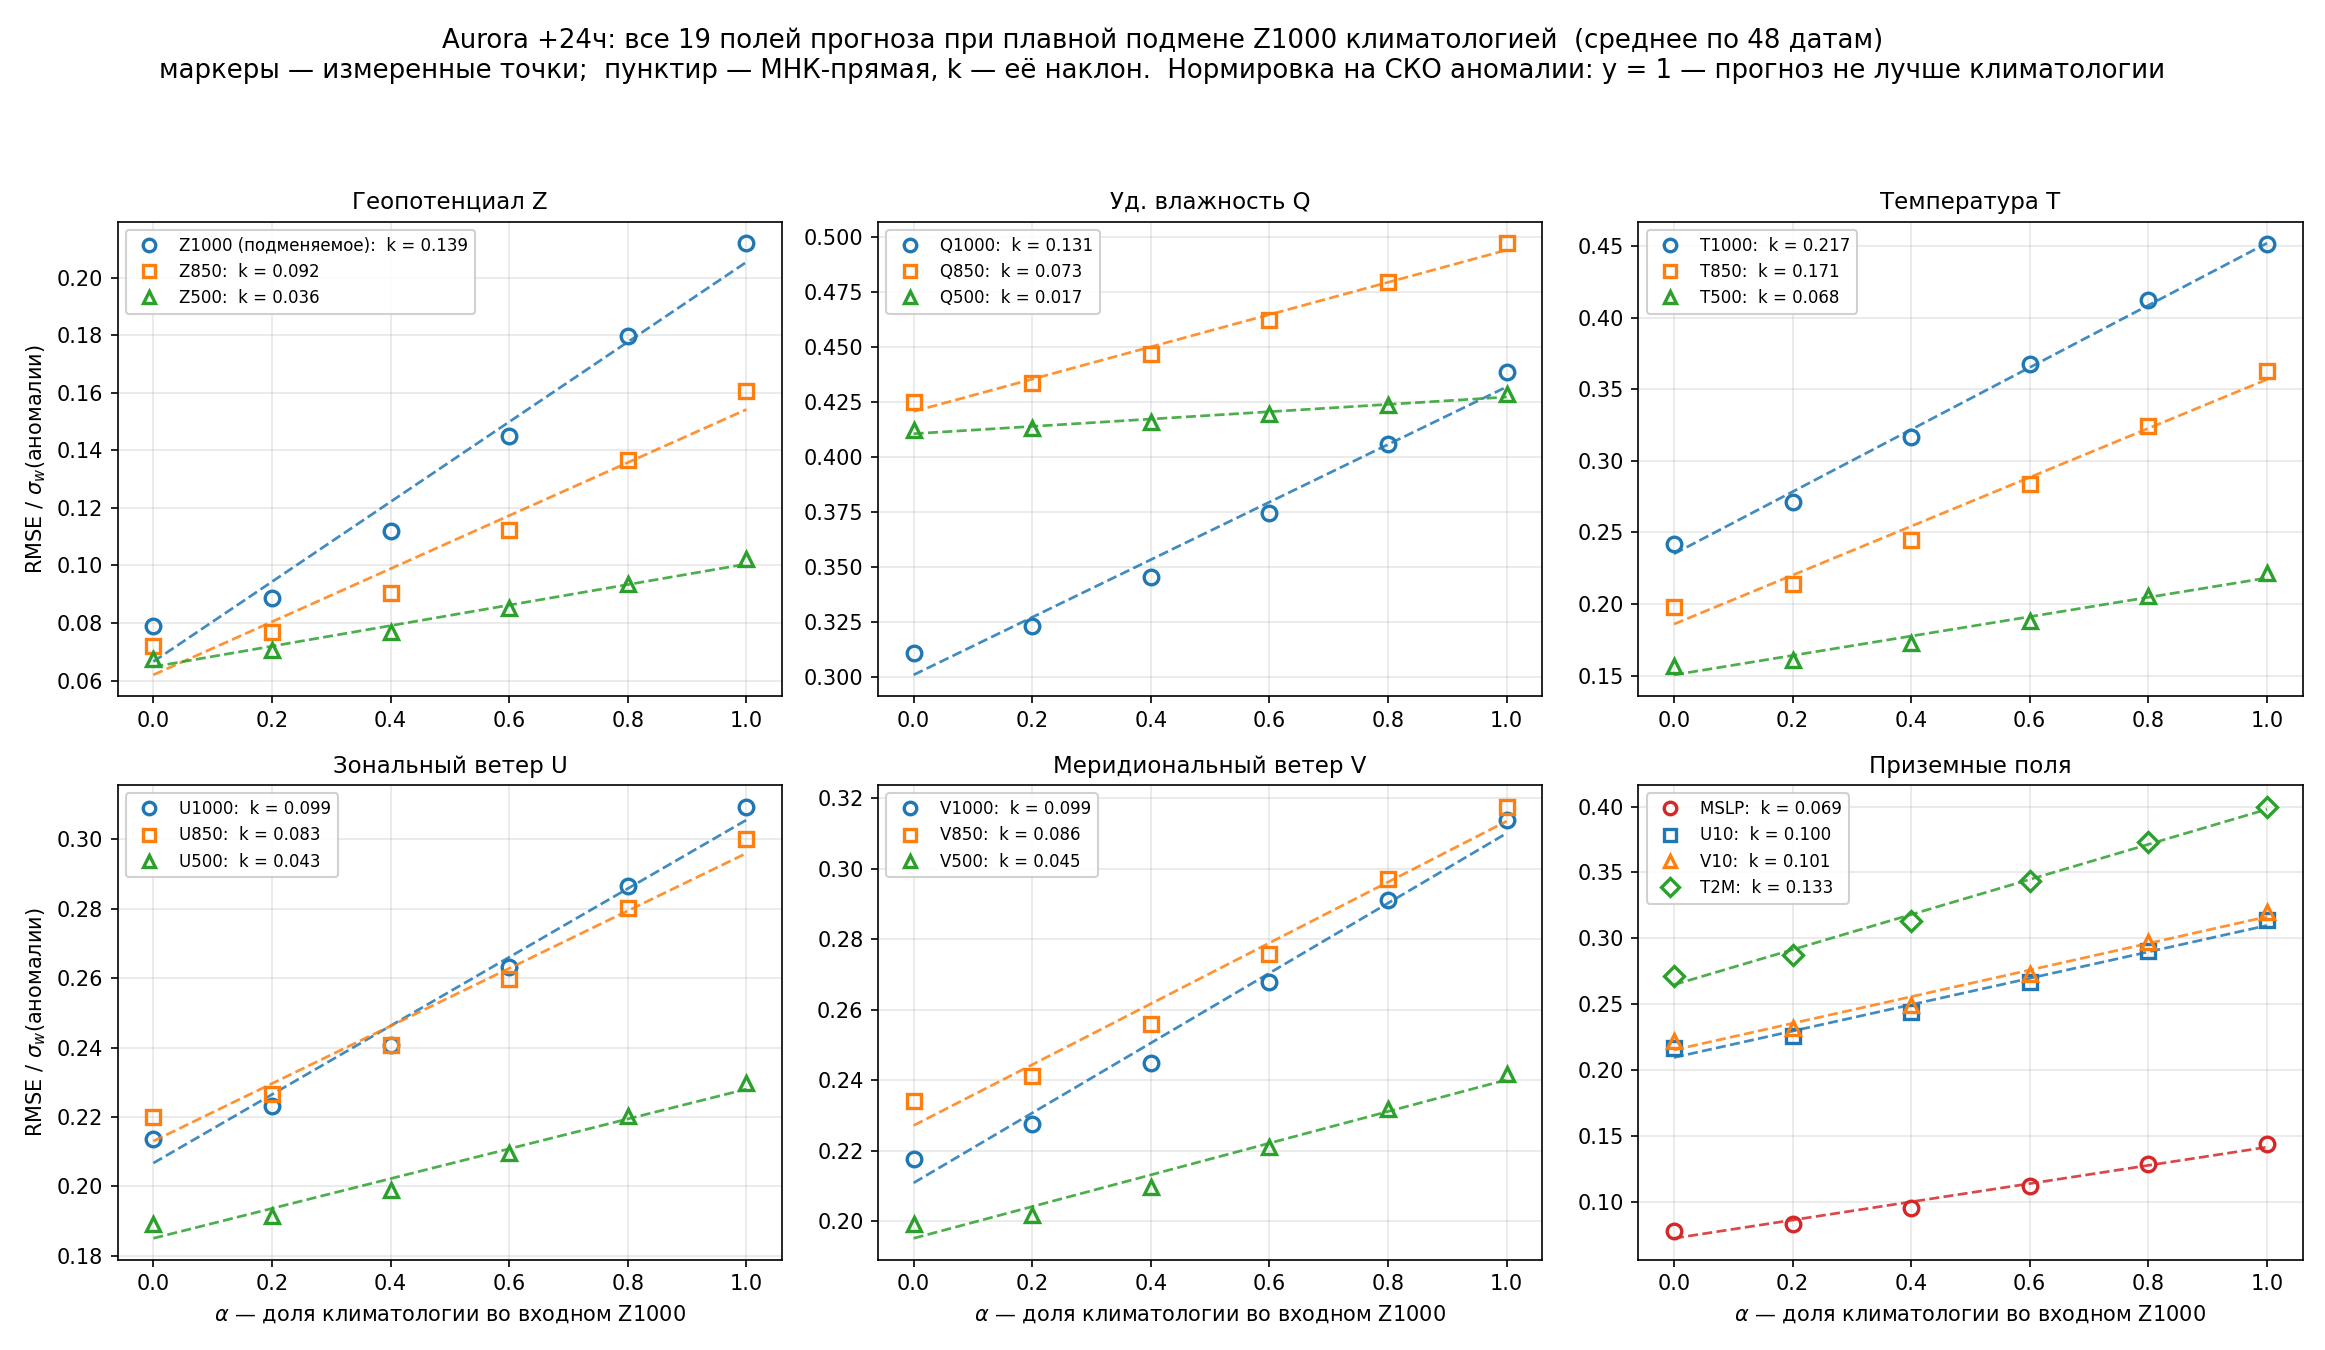
\includegraphics[width=\linewidth]{../../figures/dose_response/dose_panels_anom_Z1000_lead24_aurora_n48.png}
\caption{Aurora +24 h dose response for all 19 outputs under $Z1000$ climatology blending. The committed source panel retains its original Russian annotations.}
\end{figure}

\begin{figure}[p]
\centering
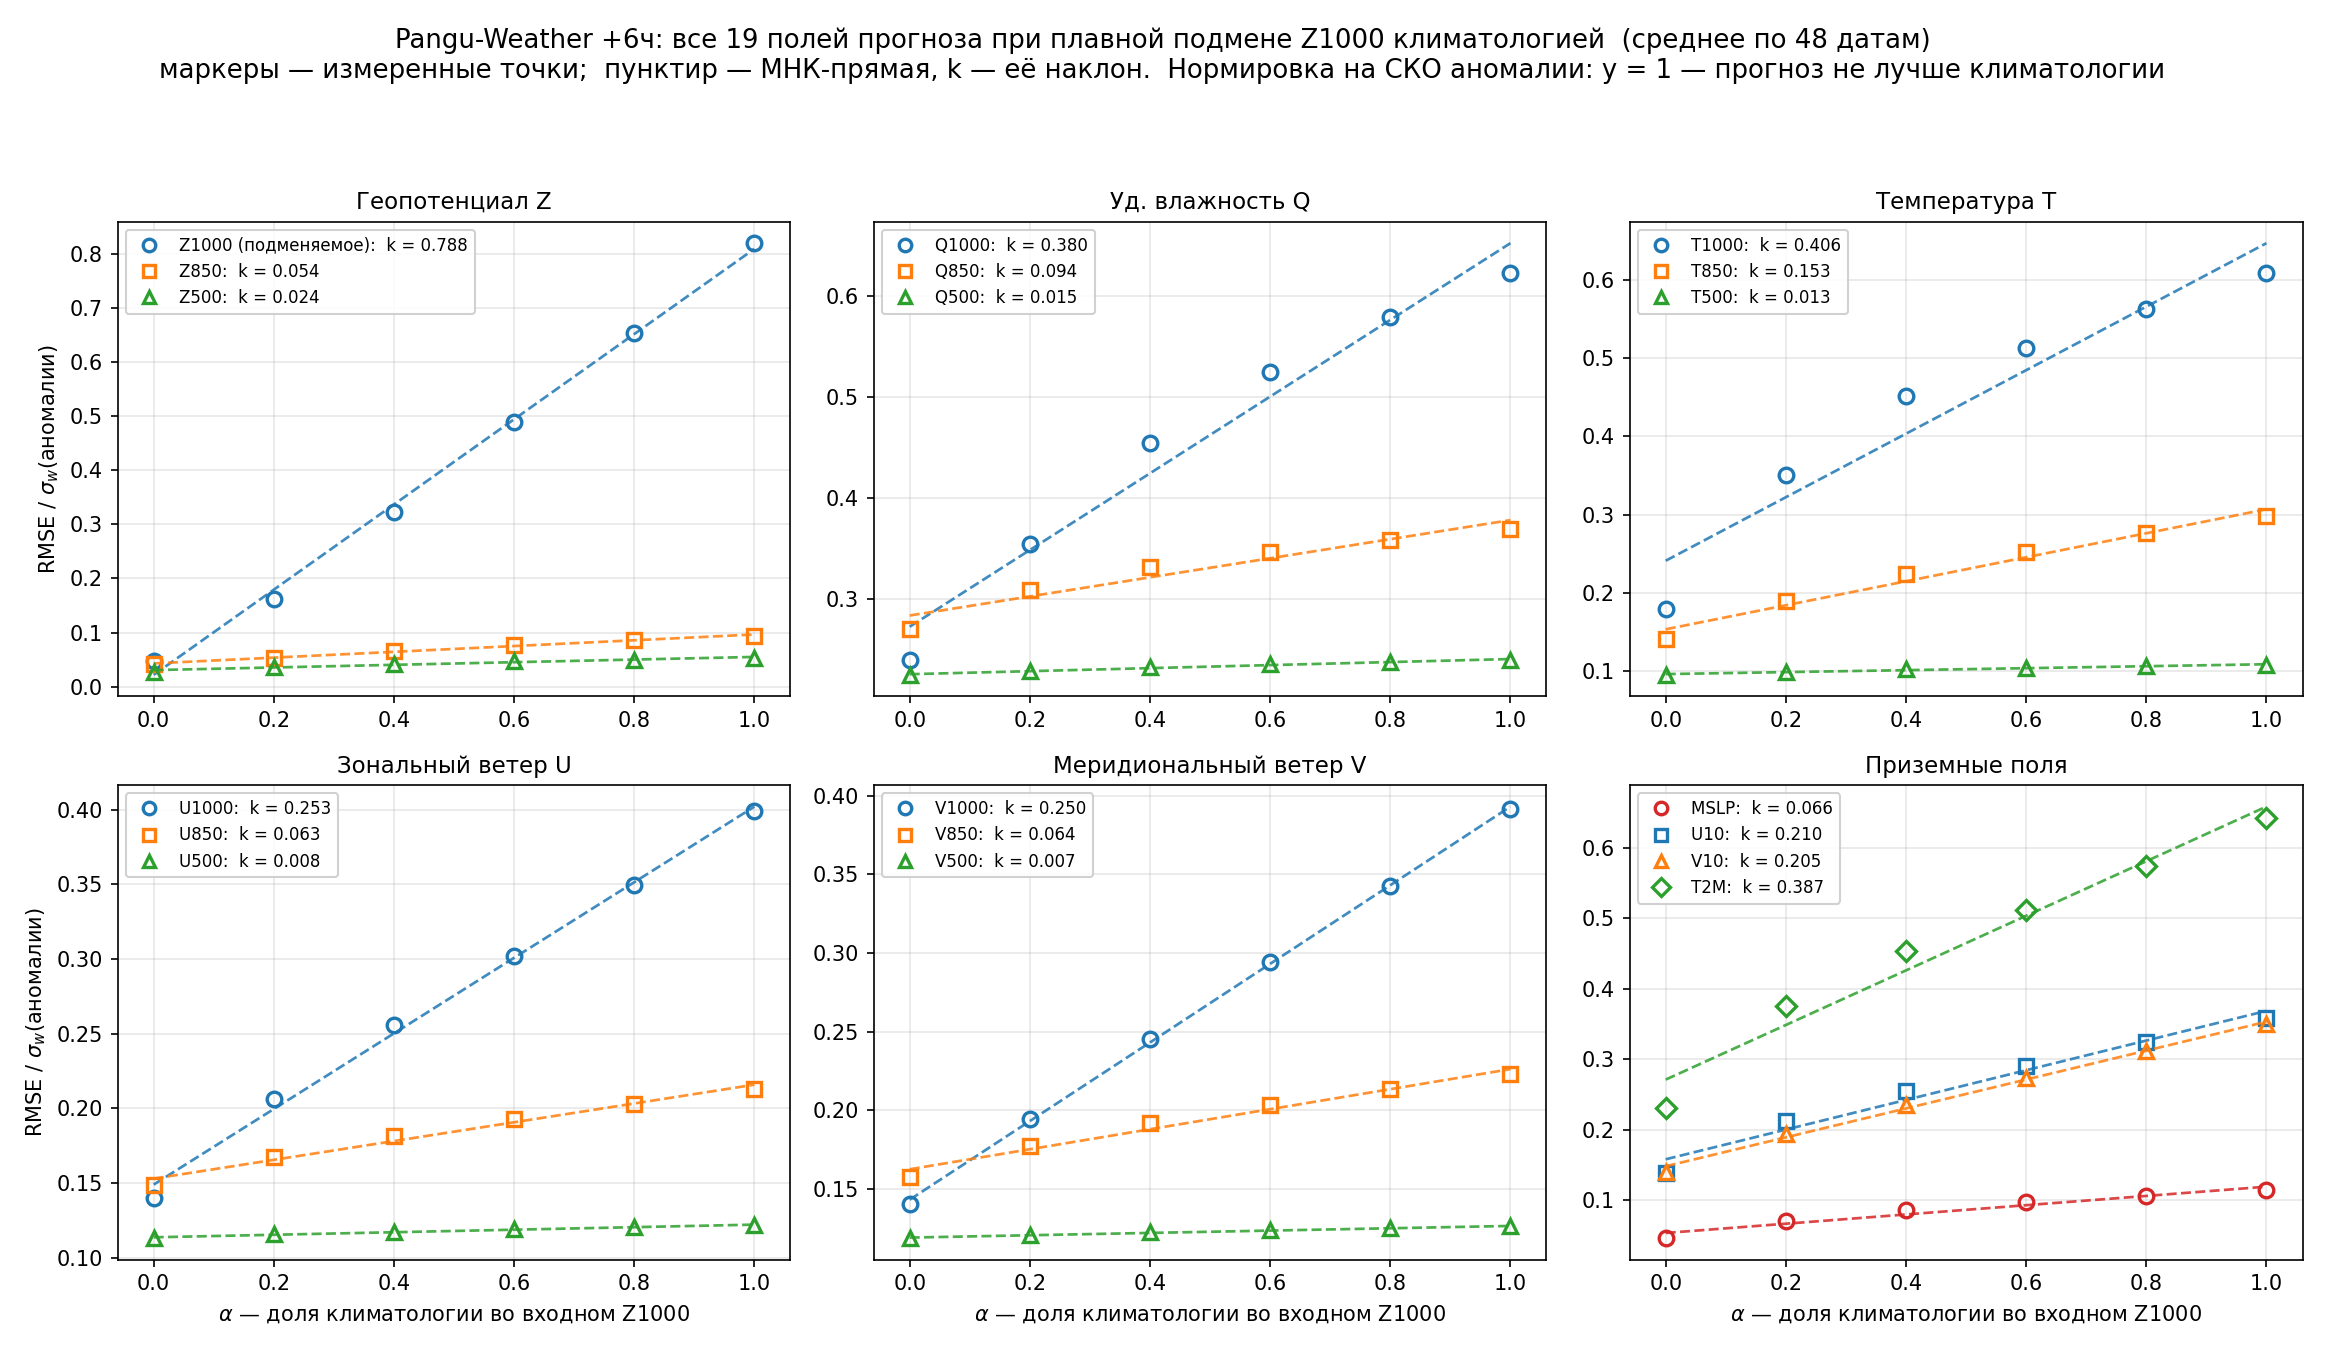
\includegraphics[width=\linewidth]{../../figures/dose_response/dose_panels_anom_Z1000_lead6_pangu_n48.png}
\caption{Pangu-Weather +6 h dose response for all 19 outputs. Pangu has a smaller $T1000$ slope than Aurora at this lead, but larger lower-level wind and $T2M$ slopes. The source annotations are in Russian.}
\end{figure}

\begin{figure}[p]
\centering
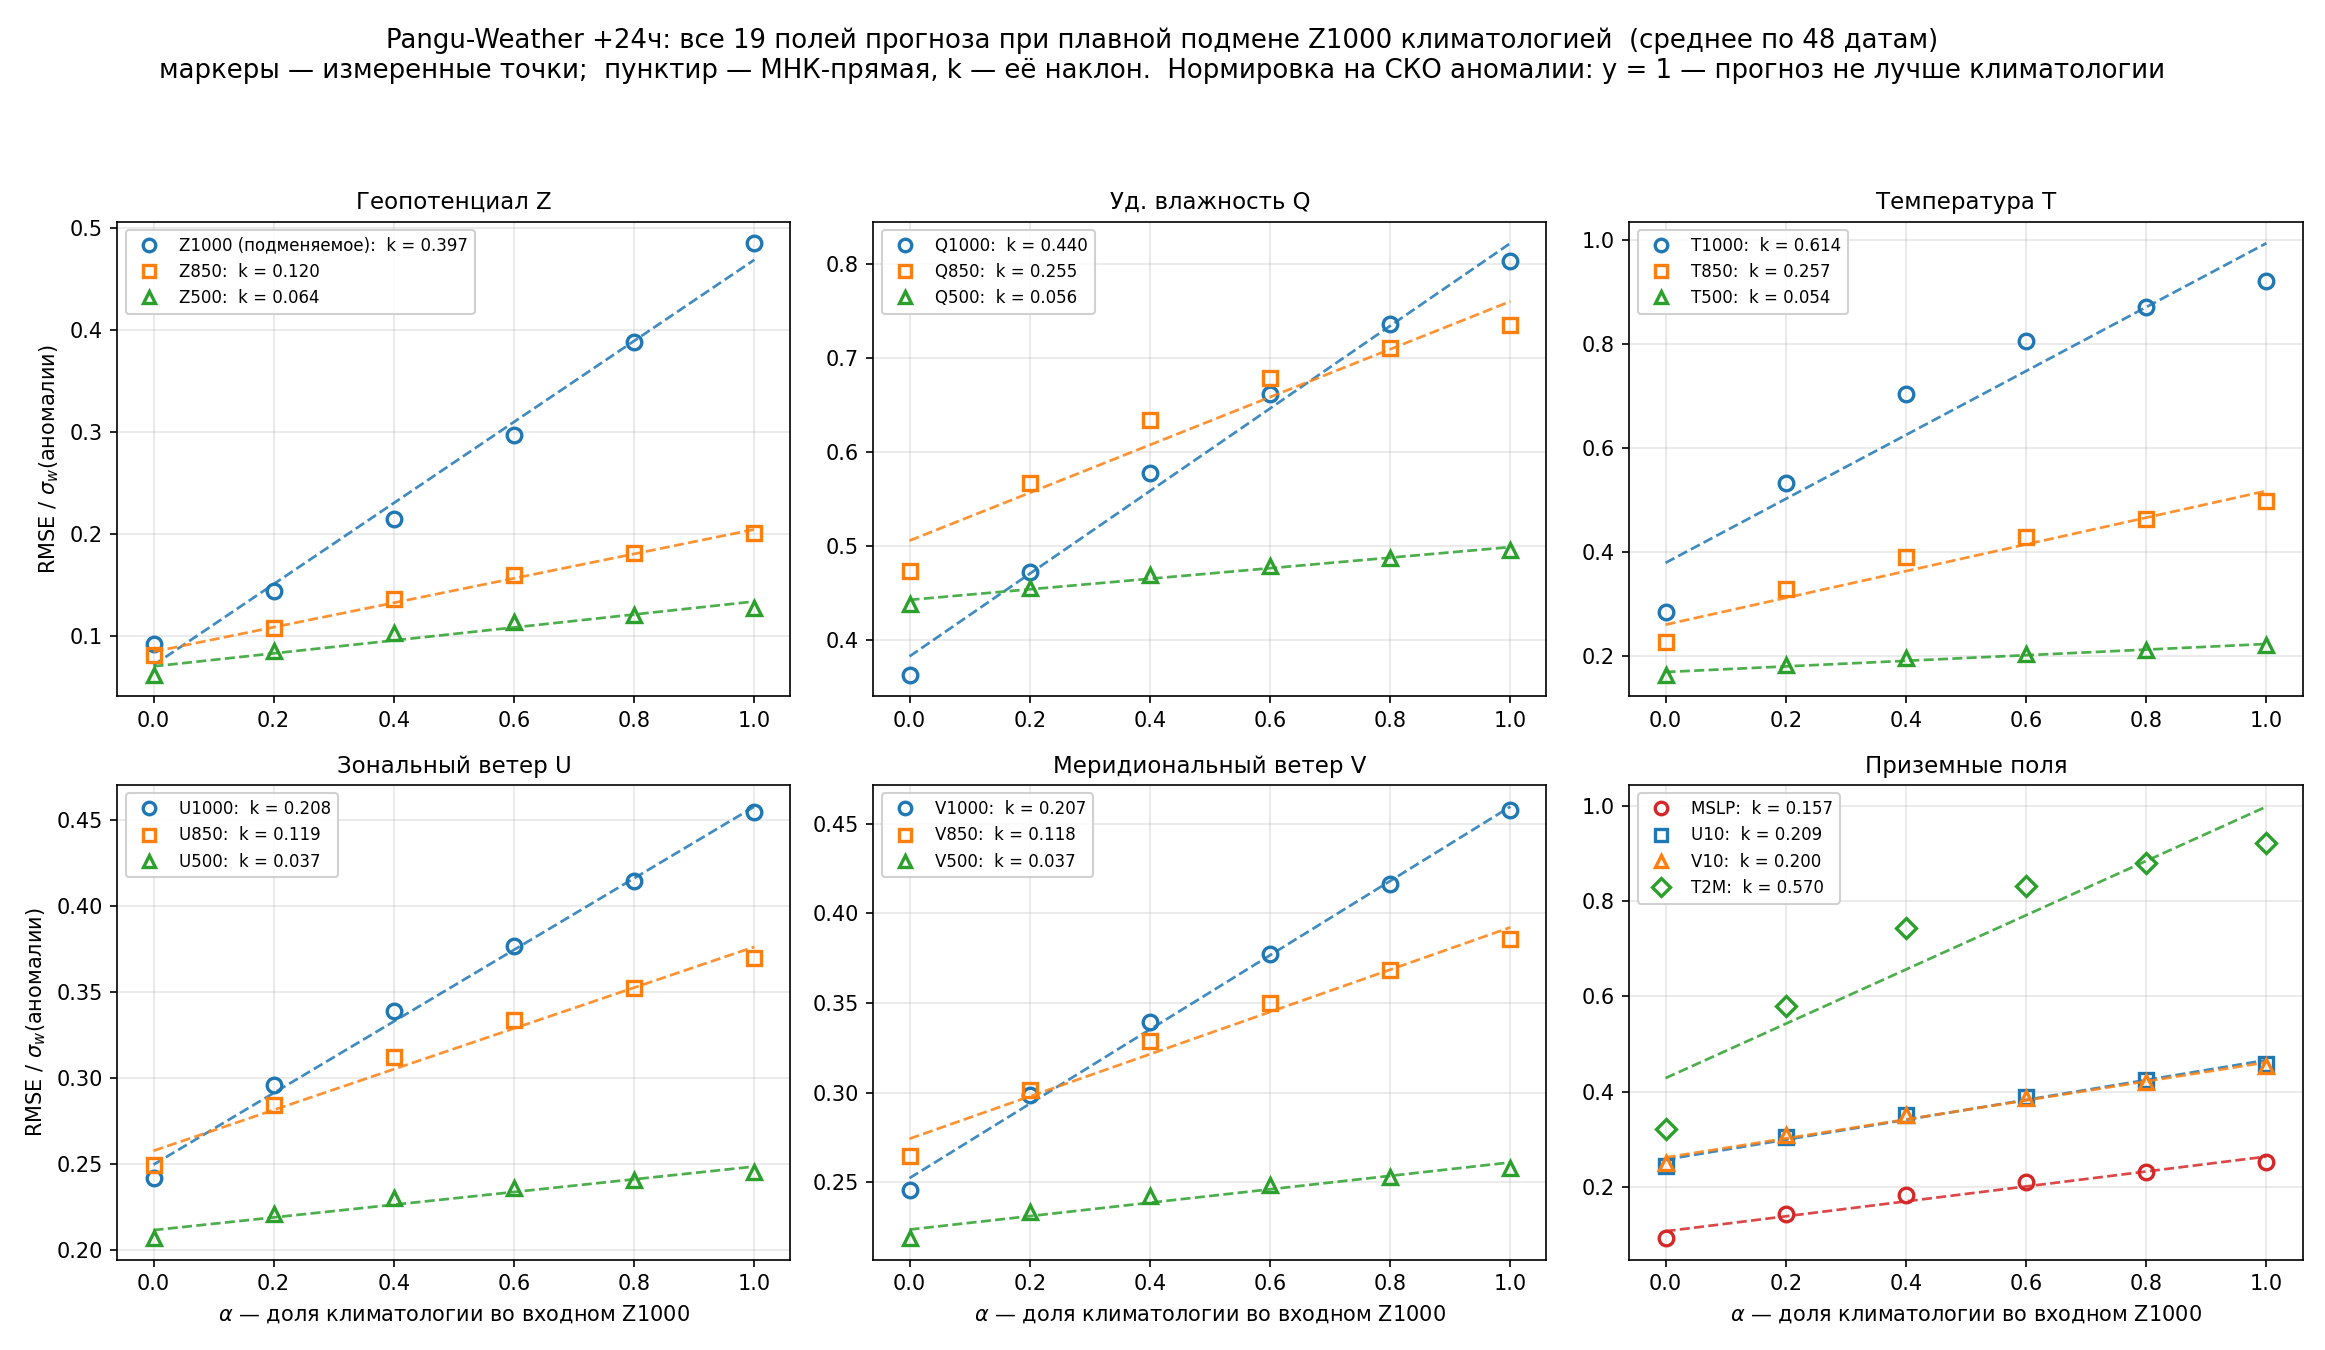
\includegraphics[width=\linewidth]{../../figures/dose_response/dose_panels_anom_Z1000_lead24_pangu_n48.png}
\caption{Pangu-Weather +24 h dose response. The $T1000$ and $T2M$ slopes increase with lead, unlike Aurora. The source annotations are in Russian.}
\end{figure}

\begin{figure}[p]
\centering
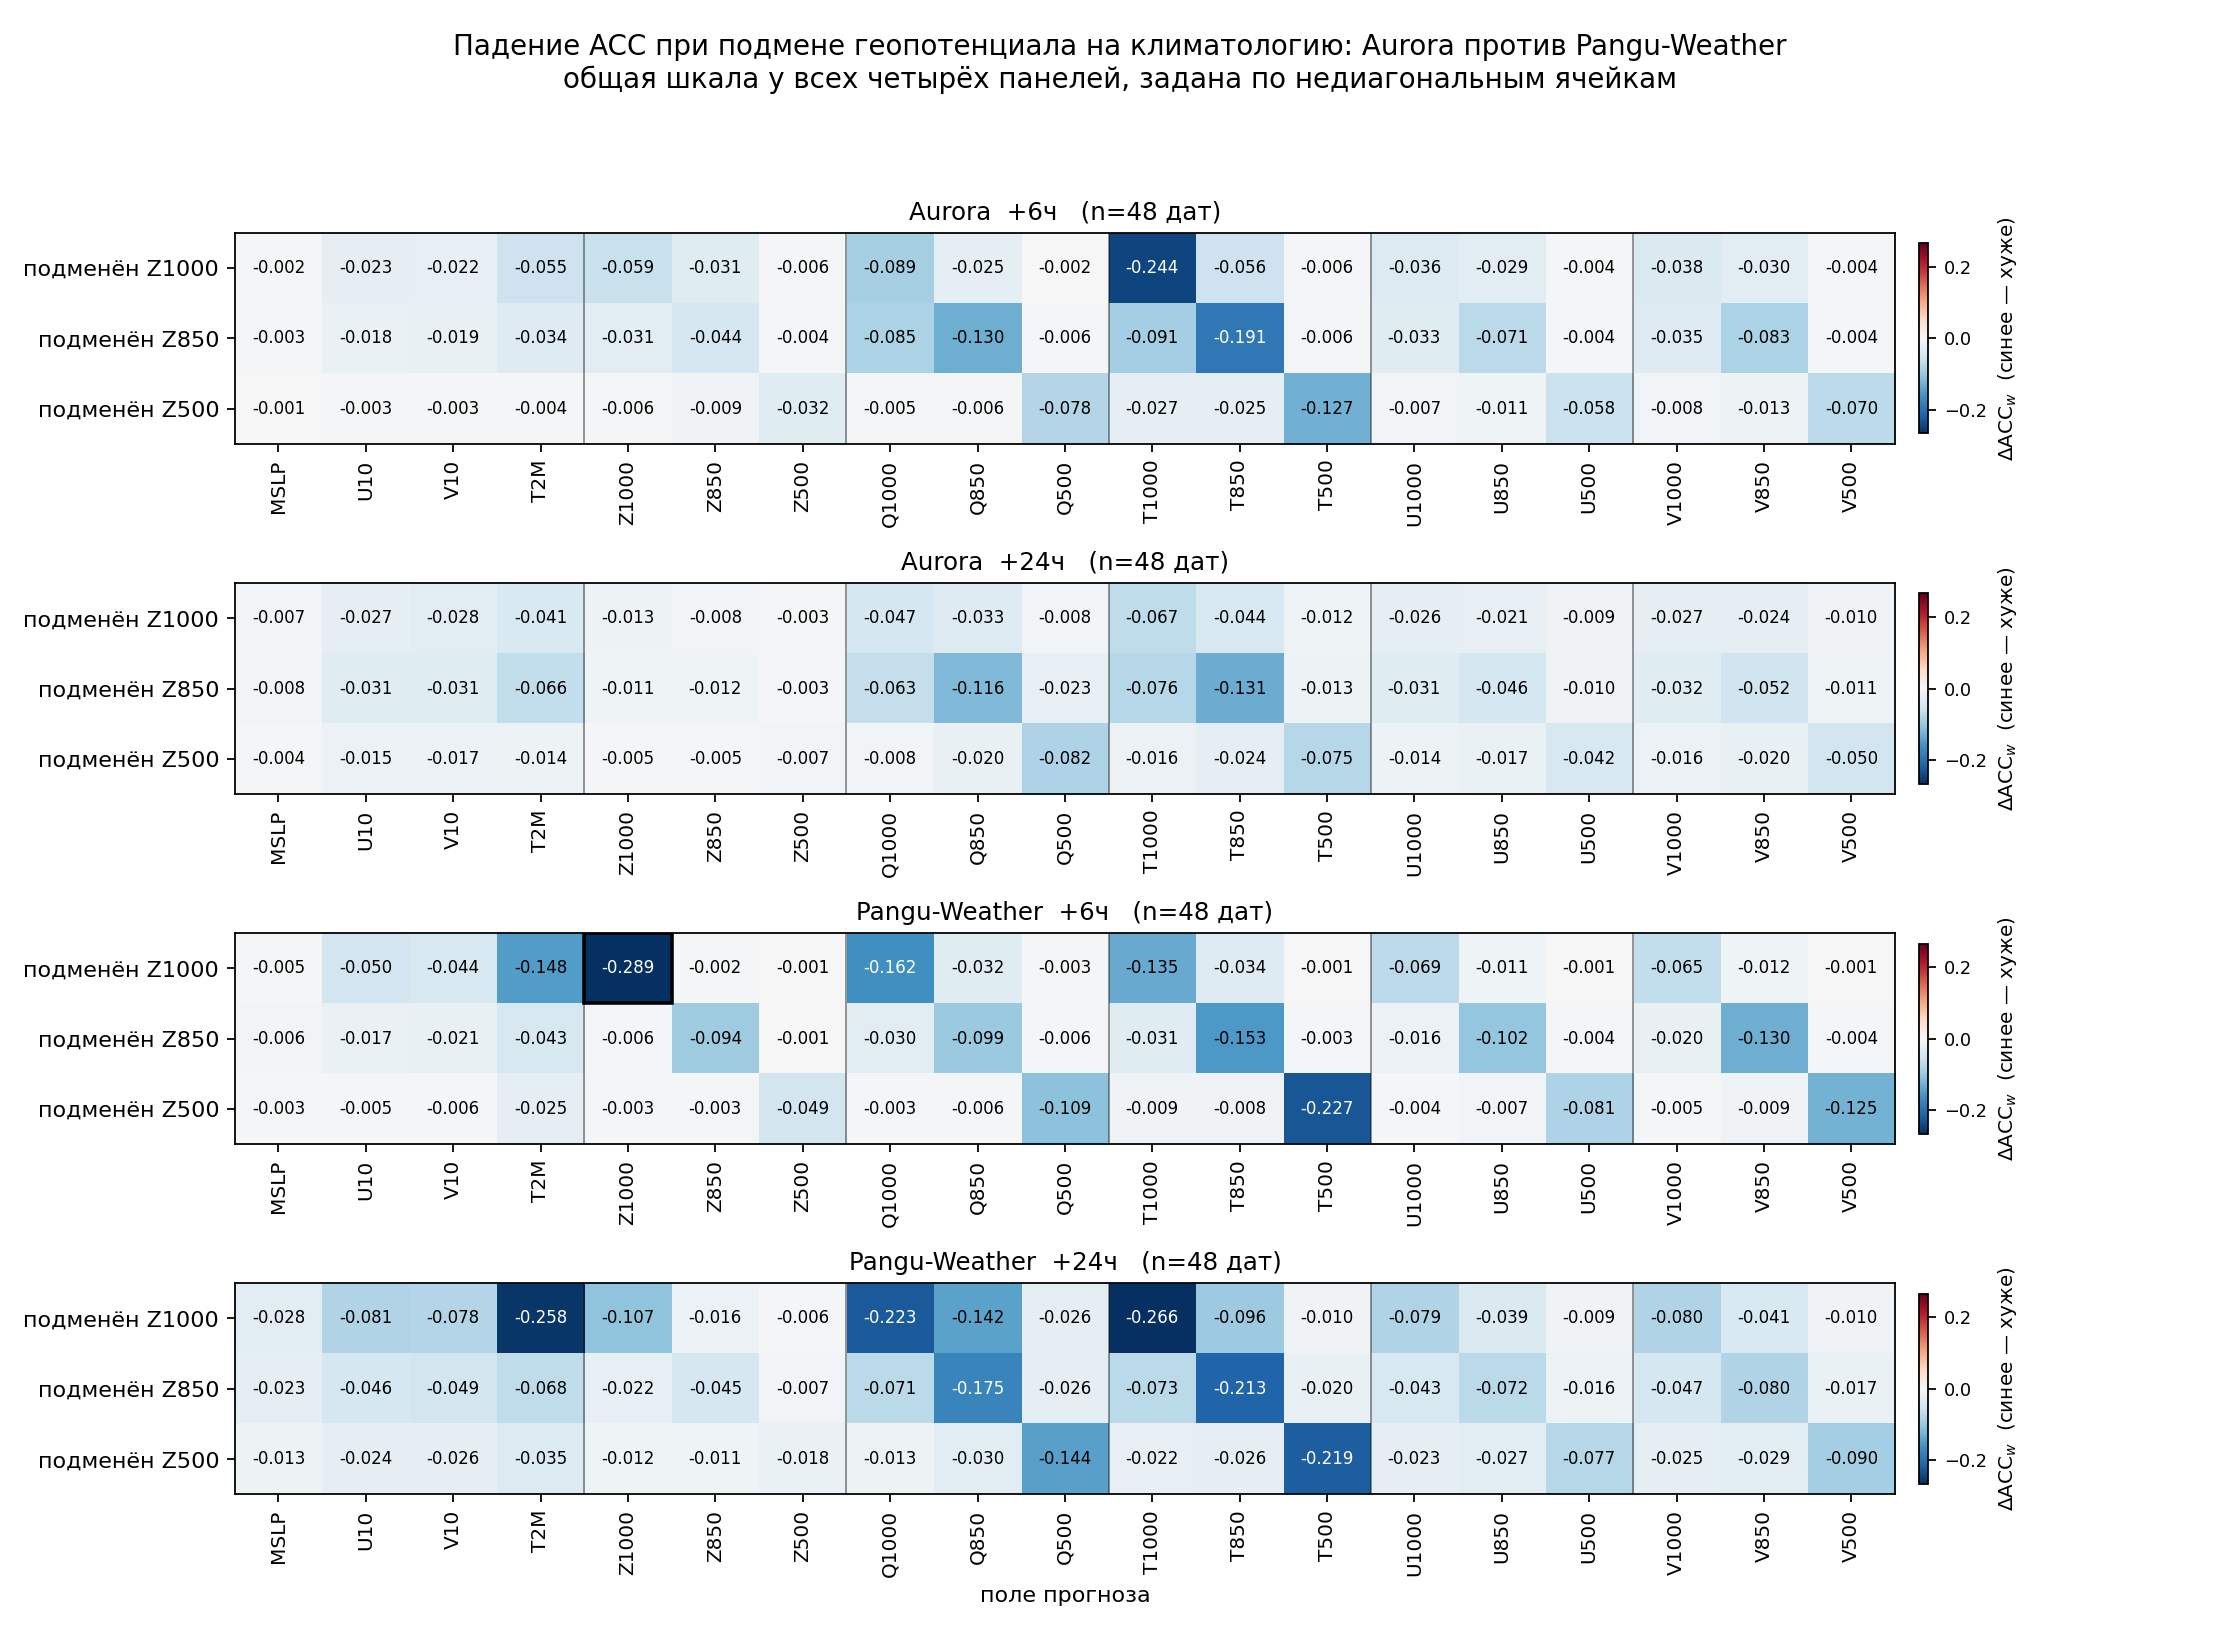
\includegraphics[width=\linewidth]{../../figures/patching_matrices/acc_strip_Z_both_n48.png}
\caption{$\Delta\acc$ rows for patching $Z1000$, $Z850$, and $Z500$ in both models. Each panel uses the scale of its parent matrix; compare the printed values rather than color saturation. The source annotations are in Russian.}
\end{figure}

\begin{figure}[p]
\centering
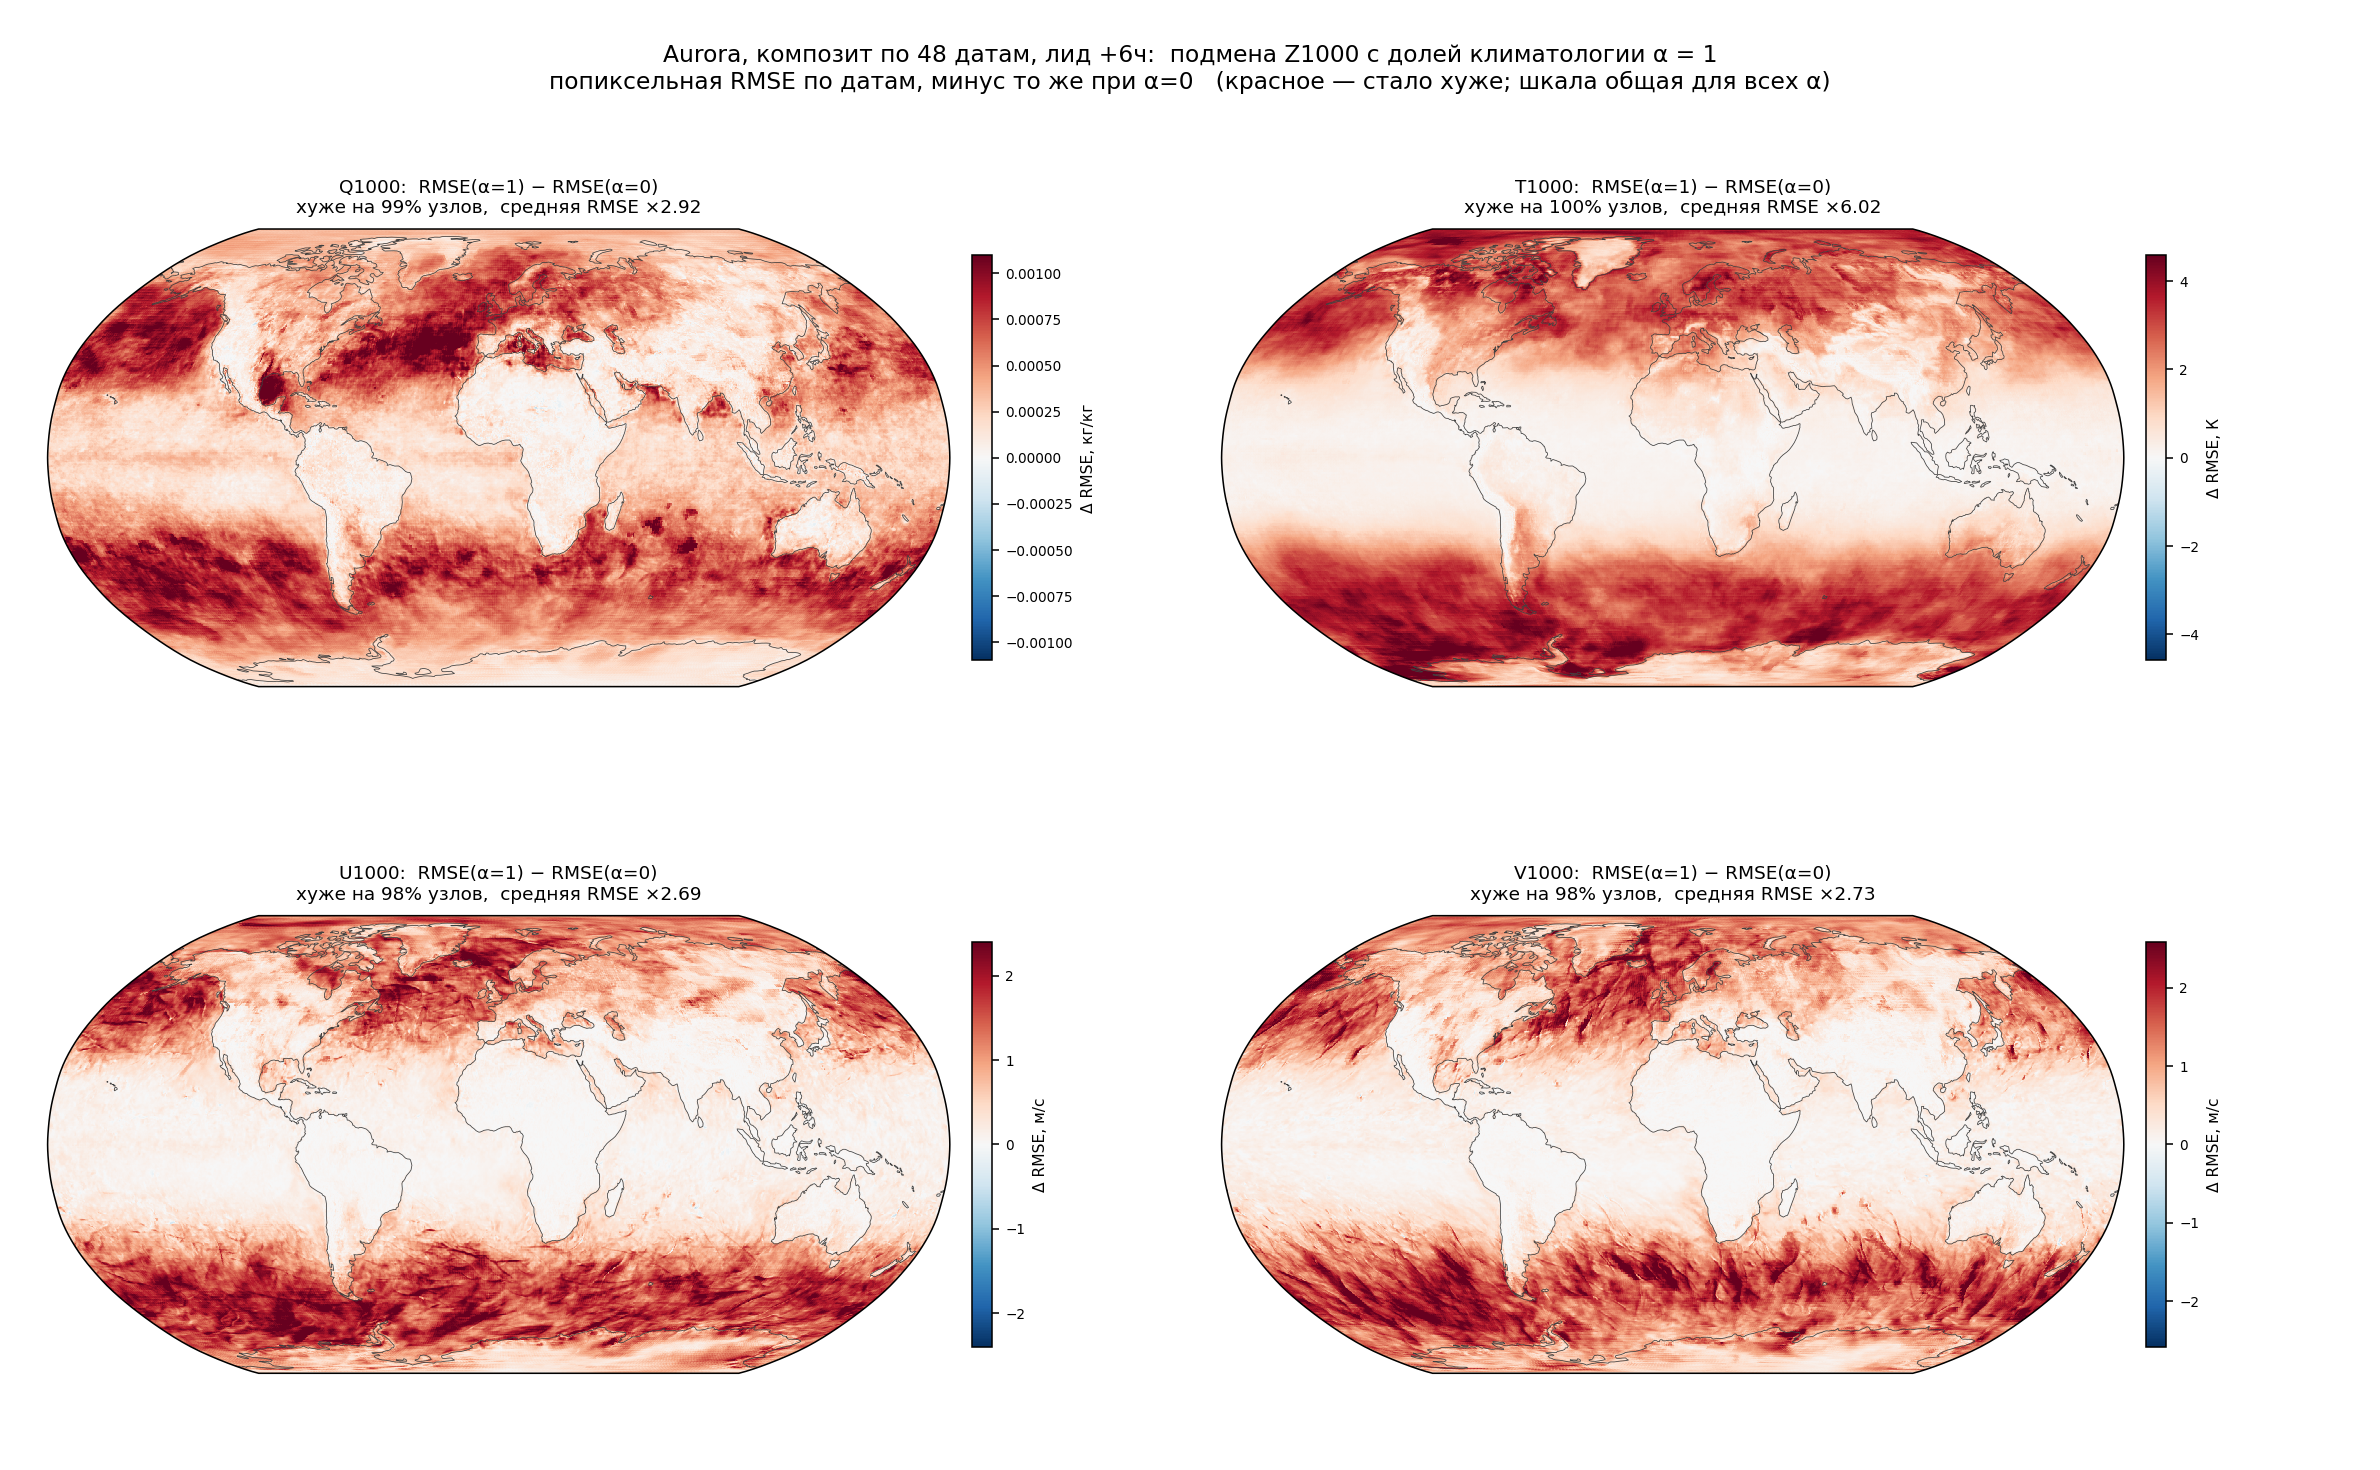
\includegraphics[width=\linewidth]{../../figures/bias_maps/composite_bias_Z1000_lead6_alpha1_n48.png}
\caption{Aurora spatial composite at full $Z1000$ replacement ($\alpha=1$, +6 h). Red denotes larger temporal RMSE than the unpatched baseline.}
\end{figure}

\begin{figure}[p]
\centering
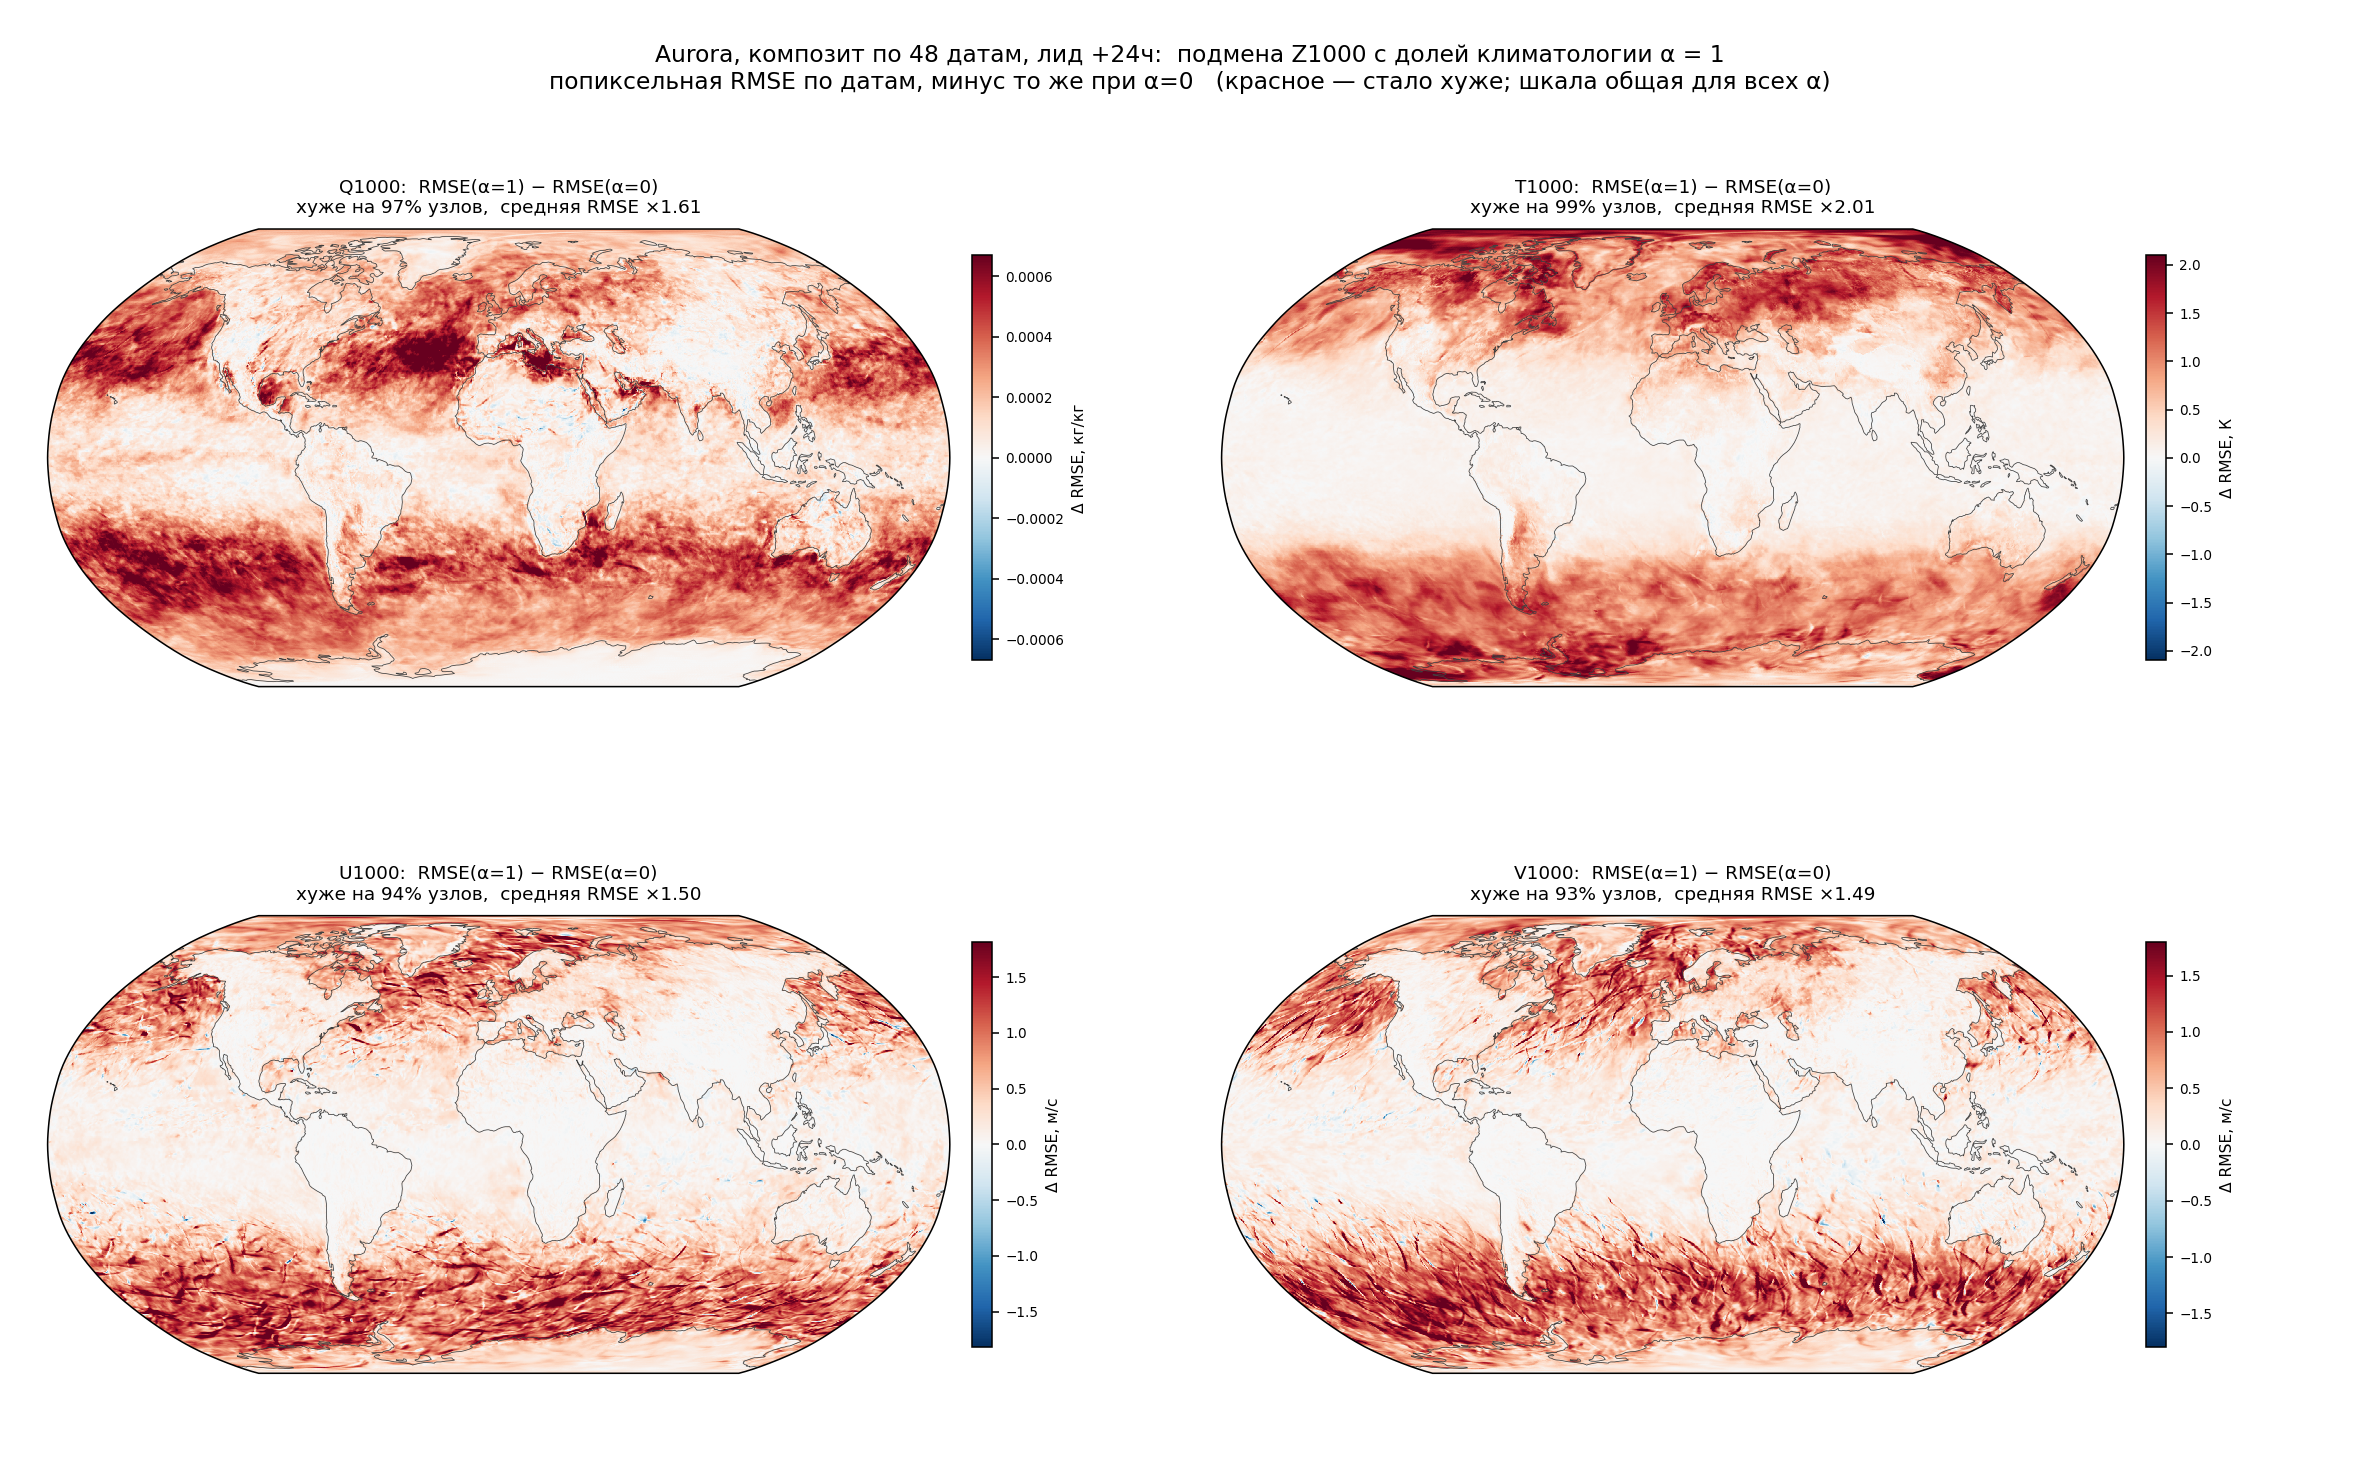
\includegraphics[width=\linewidth]{../../figures/bias_maps/composite_bias_Z1000_lead24_alpha1_n48.png}
\caption{Aurora spatial composite at +24 h. The response weakens relative to +6 h but remains positive over 93--99\% of cells for the four displayed fields.}
\end{figure}

\begin{figure}[p]
\centering
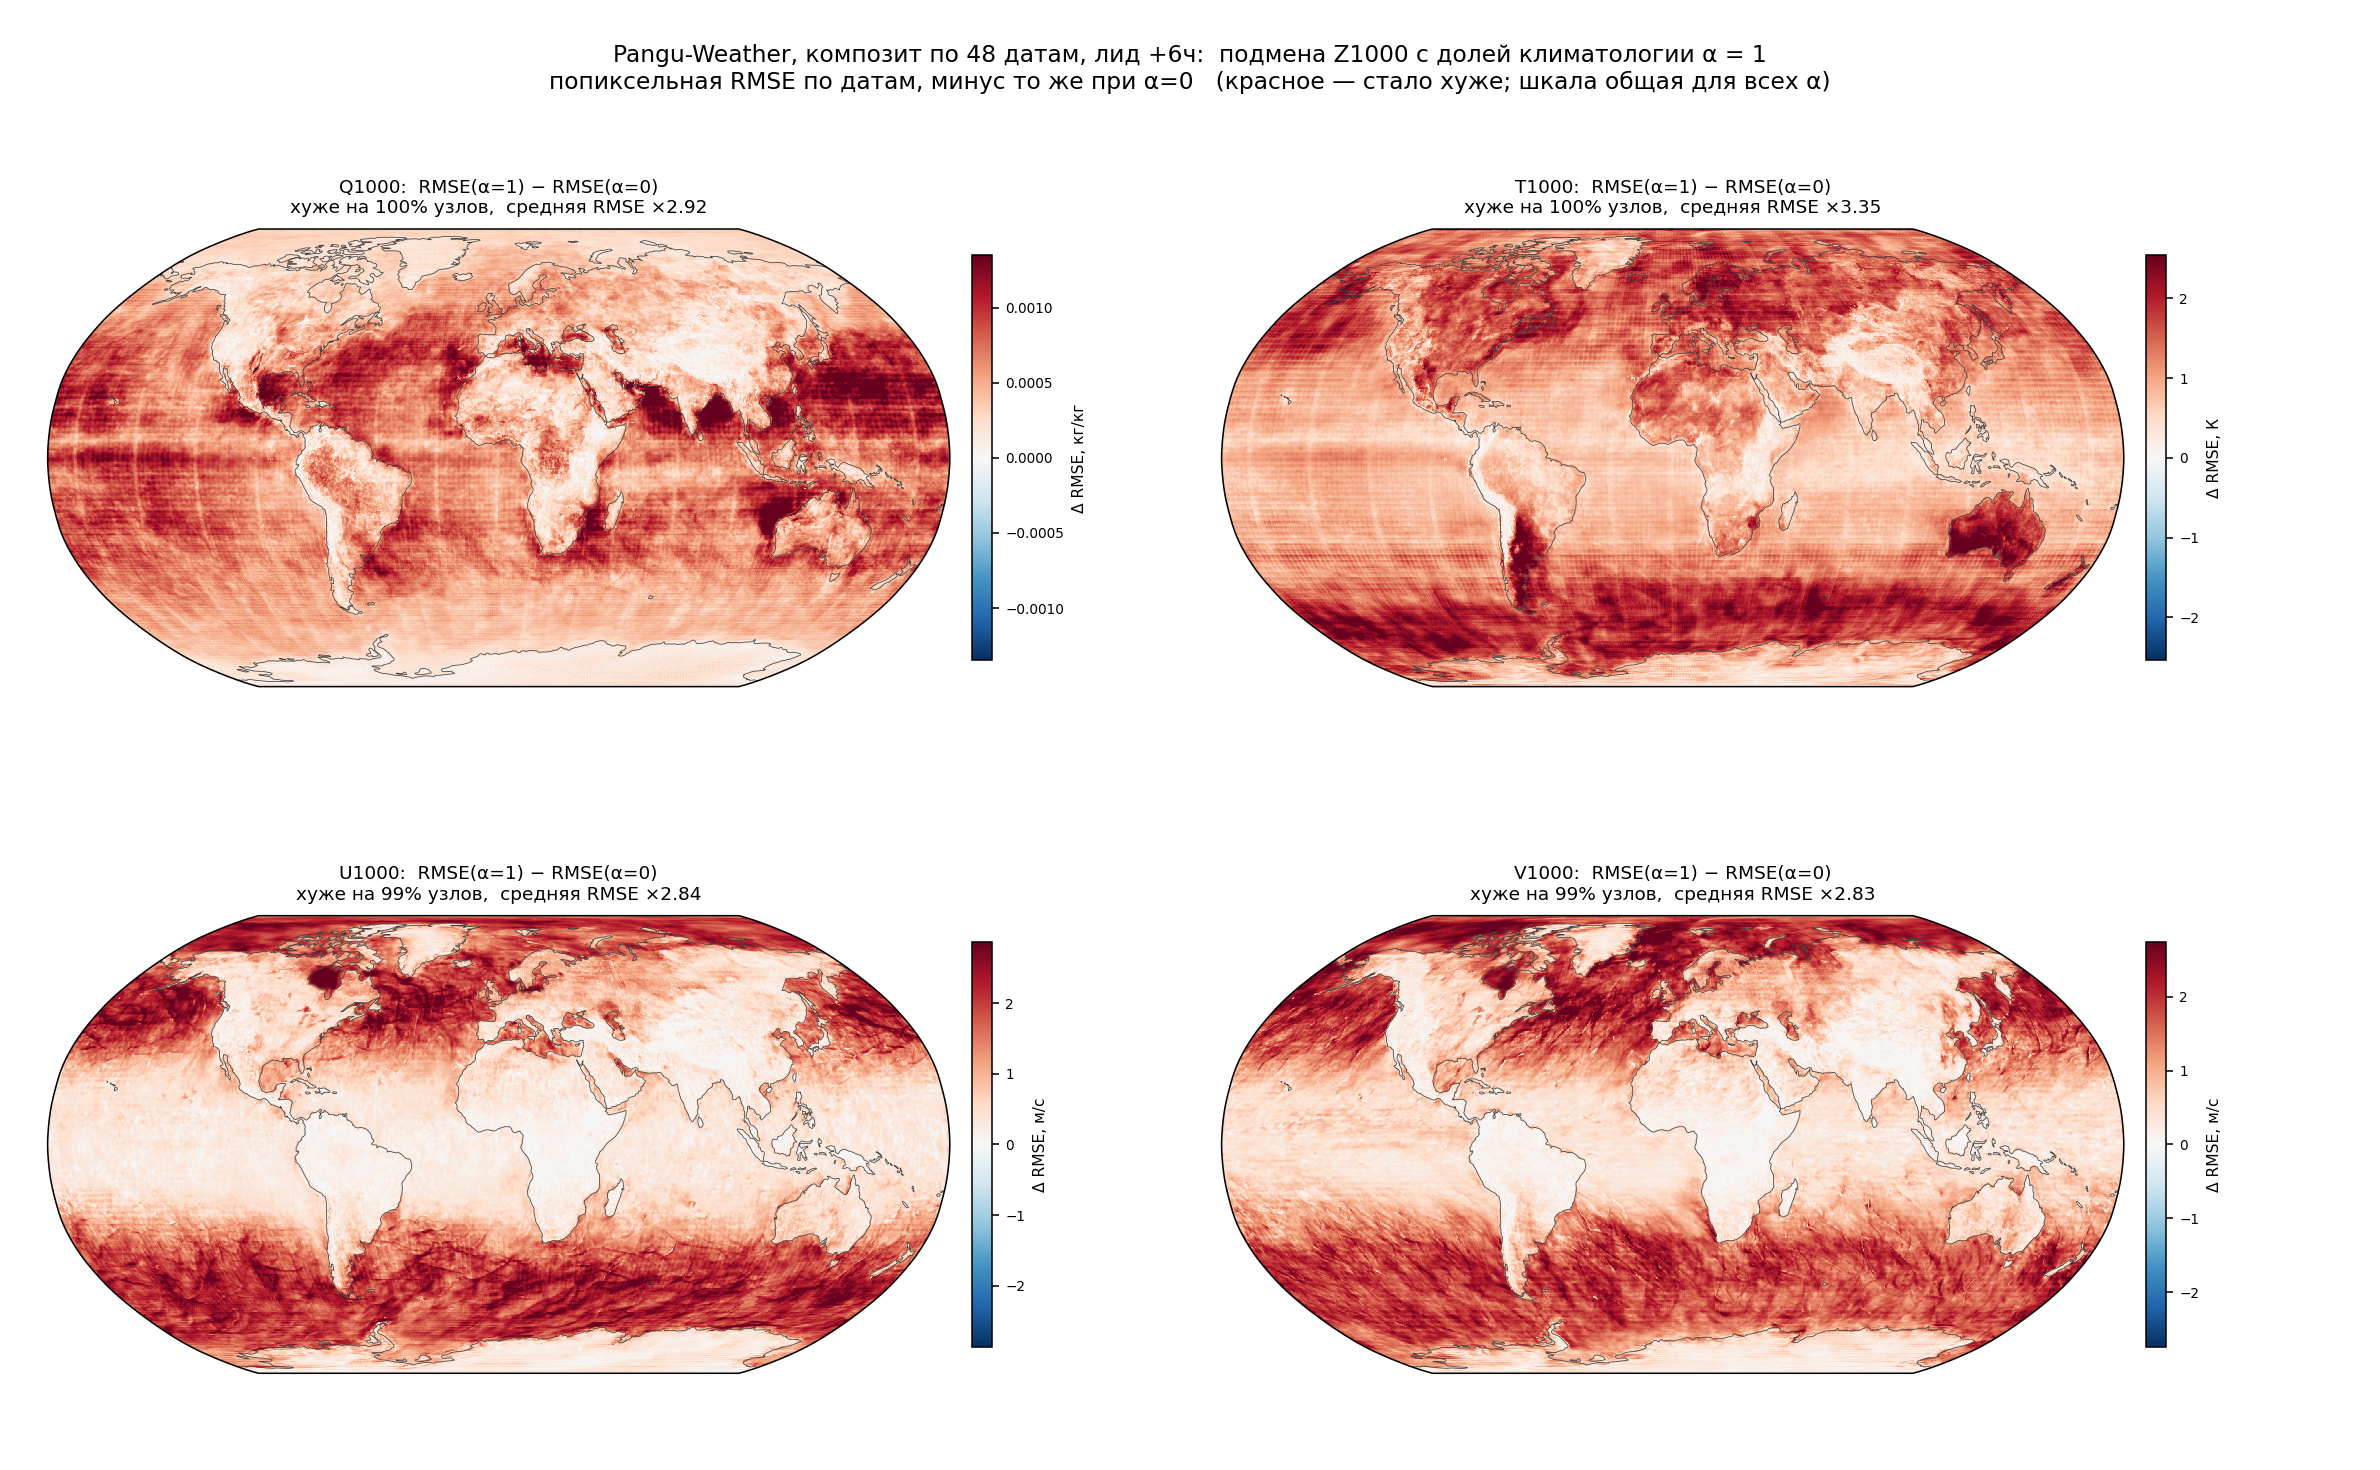
\includegraphics[width=\linewidth]{../../figures/bias_maps/composite_bias_pangu_Z1000_lead6_alpha1_n48.png}
\caption{Pangu-Weather spatial composite at +6 h. The four displayed fields worsen over 99--100\% of cells.}
\end{figure}

\begin{figure}[p]
\centering
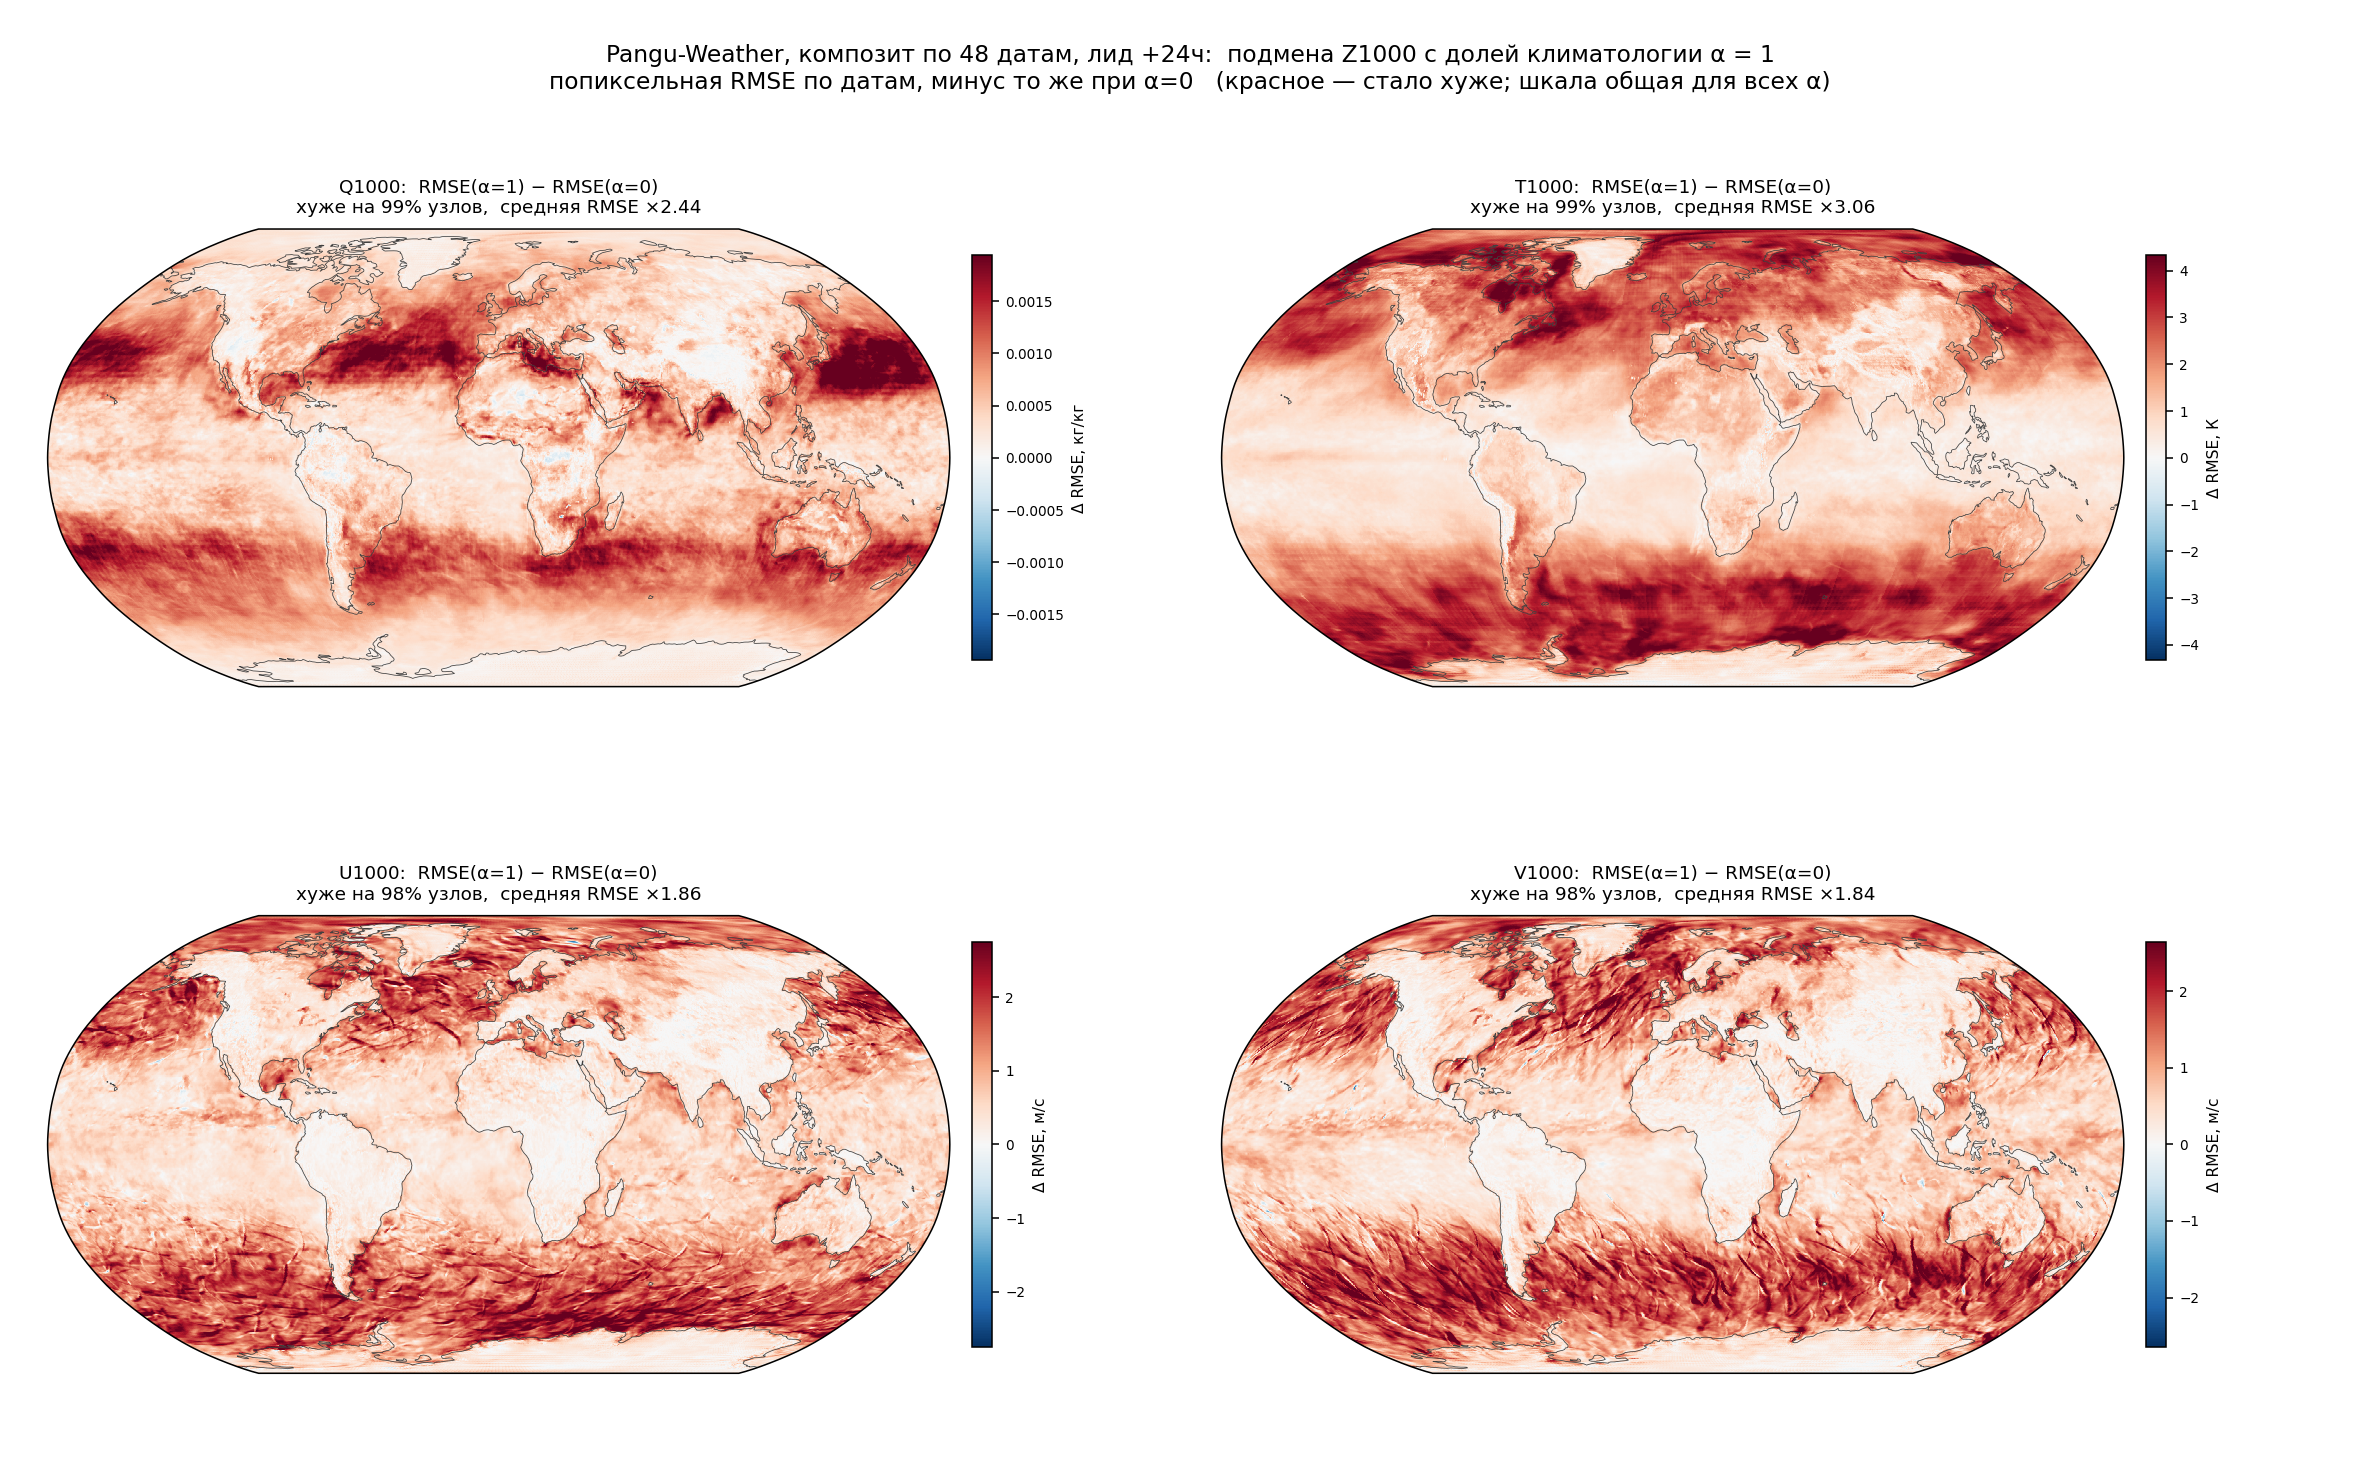
\includegraphics[width=\linewidth]{../../figures/bias_maps/composite_bias_pangu_Z1000_lead24_alpha1_n48.png}
\caption{Pangu-Weather spatial composite at +24 h. $T1000$ retains a $3.06\times$ global mean per-cell RMSE ratio, compared with $2.01\times$ for Aurora.}
\end{figure}

\end{document}
